\documentclass[a4paper]{article}
\usepackage[utf8]{inputenc}

%=-=-=-=-=-=-=-=-=-=-=-=-=-=-=-=-=-=-=-=-=-=-=-=-=-=-=-=-=-=-=-=-=-=-=-=-=-=-=-=-
% PREAMBLE
%=-=-=-=-=-=-=-=-=-=-=-=-=-=-=-=-=-=-=-=-=-=-=-=-=-=-=-=-=-=-=-=-=-=-=-=-=-=-=-=-

%%%%%%%%%%%%%%%%%%%%%%%%%%%%%%%%%%%%%%%%%%%%%%%%%%%%%%%%%%%%%%%%%%%%%
% Important styling notes
%%
% For now, to include img.jpg in img/path/to/img.jpg, just use:
% path/to/img.jpg - for details see style.tex
%=-=-=-=-=-=-=-=-=-=-=-=-=-=-=-=-=-=-=-=-=-=-=-=-=-=-=-=-=-=-=-=-=-=-=-=-=-=-=-=-
% Packages
%%
%\usepackage{fullpage} % Package to use full page
\usepackage[top=1in,bottom=1in,left=1in,right=0.7in,heightrounded]{geometry}

\usepackage{parskip}                    % Package to tweak paragraph skipping
\usepackage{amsmath}                    % standard
\usepackage{amssymb}                    % standard - Double R symbol etc.
\usepackage{hyperref}
\usepackage{amsthm}                     % standard - theorem, definition, etc.
\usepackage{multicol}                   % multiple columns for numbering
\usepackage{enumitem}                   % standard - enumerate styles
\usepackage[utf8]{inputenc}
\usepackage{scrextend}                  % indentation
\usepackage{graphicx}                   % standard - add figures
\usepackage{float}                      % standard - figure position, use [H] option
\usepackage{pifont}                     % symbols
\usepackage{gensymb}                    % degree symbol \degree
\usepackage{xcolor}                     % bg color
\hypersetup{
    colorlinks,
    linkcolor={black!50!black},
    citecolor={blue!50!black},
    urlcolor={blue!80!black}
}
\usepackage{framed}                     % bg color
\usepackage[T1]{fontenc}                % small caps
\usepackage{sectsty}                    % headings colour
\usepackage{mathtools}                  % Loads amsmath
\usepackage{amsthm,thmtools,xcolor}     % coloured theorem
\usepackage[toc,page]{appendix}         % reference to appendix
%\usepackage{titlesec}                   % change chapter, section, etc. formats
\usepackage{xifthen}                    % if, else
\usepackage{etoolbox}
% format numbering in theorem, lemma, etc. environment
\AtBeginEnvironment{theorem}{\setlist[enumerate, 1]{font=\upshape,  wide=0.5em, before=\leavevmode}}
\AtBeginEnvironment{lemma}{\setlist[enumerate, 1]{font=\upshape,  wide=0.5em, before=\leavevmode}}
\usepackage[letterspace=150]{microtype} % \textls{<letterspaced text>} % 0 <= letterspace <= 1000, 1000 = M space
\usepackage{letltxmacro}                % renew commands?
\usepackage{minted}                     % package to list code
    % otherwise minted goes off the page
    \setmintedinline{breaklines}
\usepackage{subfig}
\usepackage{eso-pic}                    % title page bg pic
\usepackage{varwidth}
\PassOptionsToPackage{svgnames}{xcolor}
\usepackage{fontawesome}                % \faQuestionCircle
\usepackage{marvosym}                   %\Pointinghand
\usepackage{mdframed}                   % easy outline frames
\usepackage[many]{tcolorbox}            % colour box for theorem styles
\usepackage{array,booktabs,calc} % table figs and text
\usepackage{comment}                    % \begin{comment}
\usepackage{fancyhdr}                   % page headings
\usepackage{mdframed}                   % boxes
\usepackage[backend=biber,sorting=none,style=ieee]{biblatex}
\usepackage{caption}
%%% caption options {
%\DeclareCaptionFont{white}{\color{white}}
\DeclareCaptionFormat{listing}{\colorbox{magenta!30!gray}{\parbox{\textwidth}{#1#2#3}}}
\captionsetup[lstlisting]{format=listing,labelfont={bf,small},textfont=small,skip=-1pt}
%%% }
\addbibresource{bibliography.bib}
\usepackage{url}
\usepackage{textcomp}
\usepackage[makeroom]{cancel}            % crossed symbols
\usepackage{algorithm}
\usepackage[noend]{algpseudocode}
\usepackage{tikz}
\usetikzlibrary{arrows.meta,positioning,quotes} % arrows and nodes in tikz
\usepackage{marginnote}
\usepackage{pgfplots}
\usepackage{pstricks-add,pst-slpe}  % for fancy tikz arrows
%\usepackage{titlesec}                   % title style
\usepackage{lmodern}                    % a font
\usepackage{titletoc} % Required for manipulating the table of contents
\usepackage{titlesec} % Allows customization of titles
\usepackage{fouriernc} % Use the New Century Schoolbook font
\usepackage{booktabs} % things in page margins
\usepackage{stmaryrd } % \varoast
\usepackage{listings} % code listings
\usepackage{longtable} % table across multiple pages
\usepackage{styles/nasm/lang}  % include custom language for NASM assembly.
\usepackage{styles/nasm/style} % include custom style for NASM assembly.



%% extra comments that I don't know where they belong:
% list of ding tags: http://willbenton.com/wb-images/pifont.pdf

%=-=-=-=-=-=-=-=-=-=-=-=-=-=-=-=-=-=-=-=-=-=-=-=-=-=-=-=-=-=-=-=-=-=-=-=-=-=-=-=-
% Colours for various things
%%


\definecolor{shadecolor}{rgb}{1.,0.933,0.96} % bg color, r,g,b <= 1
\definecolor{medium_blue}{RGB}{60,125,190}
\definecolor{dark_blue}{RGB}{25,60,85}
\definecolor{dark_red}{RGB}{77,16,16}
\definecolor{LightPink}{rgb}{0.92.,0.8,0.84} % bg color, r,g,b <= 1
\definecolor{LighterPink}{rgb}{1.,0.94,0.97} % bg color, r,g,b <= 1
\definecolor{LightestPink}{rgb}{1.,0.95,0.99} % bg color, r,g,b <= 1
\definecolor{DarkestPink}{rgb}{0.36, 0.0, 0.18}
\definecolor{DarkerPink}{rgb}{0.41, 0.0, 0.21}
\definecolor{DarkPink}{rgb}{0.55, 0.05, 0.37}
\definecolor{lightestestpink}{RGB}{255,248,252}
\definecolor{codegray}{rgb}{0.5,0.5,0.5}
\definecolor{codegrayblue}{rgb}{0.35,0.35,0.47}



%=-=-=-=-=-=-=-=-=-=-=-=-=-=-=-=-=-=-=-=-=-=-=-=-=-=-=-=-=-=-=-=-=-=-=-=-=-=-=-=-
% Define my own theorem styles
%%

% "base" styles
\declaretheoremstyle[
  headfont=\color{DarkPink}\bfseries,
  bodyfont=\itshape,
]{colored}

\declaretheoremstyle[
  headfont=\color{DarkPink}\bfseries,
  bodyfont=\normalfont,
]{colored_upright}

% theorems (corollaries, etc) themselves, inherit from my style above
% Usage:
% \begin{theorem} \end{theorem}, \begin{lemma} \end{lemma}, ...
\declaretheorem[
	numberwithin=section,
 	style=colored,
	name=\textsc{Theorem},
]{theorem}

\tcolorboxenvironment{theorem}{
  boxrule=0pt,
  boxsep=2pt,
  colback={magenta!25!white},
  colframe=DarkPink,
  enhanced jigsaw, 
  borderline west={2pt}{0pt}{DarkPink},
  sharp corners,
  before skip=5pt,
  after skip=5pt,
  breakable,
  right=0mm % for equations
}

\declaretheorem[
	numberwithin=section,
 	style=colored,
	name=\textsc{Corollary},
]{corollary}

\tcolorboxenvironment{corollary}{
  boxrule=0pt,
  boxsep=1pt,
  colback={magenta!10!white},
  colframe=DarkPink,
  enhanced jigsaw, 
  borderline west={2pt}{0pt}{DarkPink},
  sharp corners,
  before skip=5pt,
  after skip=5pt,
  breakable,
  right=0mm % for equations
}

\declaretheorem[
	numberwithin=section,
	style=colored,
	name=\textsc{Lemma},
]{lemma}

\tcolorboxenvironment{lemma}{
  boxrule=0pt,
  boxsep=1pt,
  colback={magenta!10!white},
  colframe=DarkPink,
  enhanced jigsaw, 
  borderline west={2pt}{0pt}{DarkPink},
  sharp corners,
  before skip=5pt,
  after skip=5pt,
  breakable,
  right=0mm % for equations
}

\declaretheorem[
	numberwithin=section,
	style=colored,
	name=\textsc{Definition},
]{definition}

\tcolorboxenvironment{definition}{
  boxrule=0pt,
  boxsep=1pt,
  colback={magenta!25!white},
  colframe=DarkPink,
  enhanced jigsaw, 
  borderline west={2pt}{0pt}{DarkPink},
  sharp corners,
  before skip=5pt,
  after skip=5pt,
  breakable,
  right=0mm % for equations
}

\declaretheorem[
	numberwithin=section,
  	style=colored,
  	name=\textsc{Example},
]{exmp}

\declaretheorem[
	numberwithin=section,
  	style=colored,
  	name=\textsc{Solution},
]{soln}

%%% code listings
\lstdefinestyle{code1}{
    backgroundcolor=\color{lightestestpink},   
    commentstyle=\color{codegrayblue},
    keywordstyle=\color{DarkerPink},
    numberstyle=\tiny\color{codegray},
    stringstyle=\color{black!40!cyan},
    basicstyle=\small\ttfamily,
    breakatwhitespace=false,
    breaklines=true,        
    captionpos=t,             
    keepspaces=true,        
    numbers=left,           
    numbersep=5pt,
    showspaces=false, 
    showstringspaces=false,
    showtabs=false,
    tabsize=4
}

\lstset{style=code1}

%=-=-=-=-=-=-=-=-=-=-=-=-=-=-=-=-=-=-=-=-=-=-=-=-=-=-=-=-=-=-=-=-=-=-=-=-=-=-=-=-
% Headers (size, font, colour)
%%




\makeatletter
\renewcommand{\@seccntformat}[1]{\llap{\textcolor{DarkestPink}{\csname the#1\endcsname}\hspace{1em}}}                    
\renewcommand{\section}{\@startsection{section}{1}{\z@}
{-4ex \@plus -1ex \@minus -.4ex}
{1ex \@plus.2ex }
{\normalfont\large\sffamily\bfseries\textcolor{DarkestPink}}}
\renewcommand{\subsection}{\@startsection {subsection}{2}{\z@}
{-3ex \@plus -0.1ex \@minus -.4ex}
{0.5ex \@plus.2ex }
{\normalfont\sffamily\bfseries\textcolor{DarkestPink}}}
\renewcommand{\subsubsection}{\@startsection {subsubsection}{3}{\z@}
{-2ex \@plus -0.1ex \@minus -.2ex}
{.2ex \@plus.2ex }
{\normalfont\small\sffamily\bfseries\textcolor{DarkestPink}}}                        


%=-=-=-=-=-=-=-=-=-=-=-=-=-=-=-=-=-=-=-=-=-=-=-=-=-=-=-=-=-=-=-=-=-=-=-=-=-=-=-=-
% Numberings, counters and spacings
%%
\numberwithin{equation}{section} % section number in eq/s
\setlength{\jot}{7pt} % spacing in split, gathered env/s



%% Custom examples
%% Output - Example 1,2,...
\newcounter{example}
\newenvironment{example}[1][]{\refstepcounter{example}\par\medskip
   \textbf{Example~\theexample. #1} \rmfamily}{\medskip}
%%%%%%%%%%%% End of unused %%%%%%%%%%%%



%=-=-=-=-=-=-=-=-=-=-=-=-=-=-=-=-=-=-=-=-=-=-=-=-=-=-=-=-=-=-=-=-=-=-=-=-=-=-=-=-
% Paths
%%
\graphicspath{ {./img/} } % figures' path - can look up files directly from there


%=-=-=-=-=-=-=-=-=-=-=-=-=-=-=-=-=-=-=-=-=-=-=-=-=-=-=-=-=-=-=-=-=-=-=-=-=-=-=-=-
% User defined macros (math mode)
%%


% Curly braces under text. Usage: \myunderbrace{upper}{lower}
\newcommand{\myunderbrace}[2]{\mathrlap{\underbrace{\phantom{#1}}_{#2}} #1}
\newcommand{\setR}{\mathbb{R}} % \ouble R
\newcommand{\setRn}{\mathbb{R}^n} %  double R^n
\newcommand{\setN}{\mathbb{N}} % double N
\newcommand{\setZ}{\mathbb{Z}} % double Z
\let\oldemptyset\emptyset
\let\emptyset\varnothing % nice - looking empty set symbol
\newcommand{\fancyN}{\mathcal{N}} % null space
\newcommand{\fancyR}{\mathcal{R}} % range

\newcommand{\bx}{\textbf{x}}
\newcommand{\by}{\textbf{y}}
\newcommand{\bb}{\textbf{b}}
\newcommand{\bA}{\textbf{A}}
\newcommand{\bB}{\textbf{B}}
\newcommand{\bI}{\textbf{I}}
% double bars as in norm
\newcommand{\norm}[1] {\lVert #1 \rVert} 
\newcommand{\trans}[1]{#1^{\top}}

\newcommand{\mean}[1]{\bar{#1}}
\newcommand{\var}{\sigma^2}

\newcommand{\partdevx}[1]{\frac{\partial #1}{\partial x}}
\newcommand{\partdevxx}[1]{\frac{\partial #1}{\partial x}}
\newcommand{\partdevxn}[1]{\frac{\partial^n #1}{\partial x^n}}
\newcommand{\partdevy}[1]{\frac{\partial #1}{\partial x}}
\newcommand{\partdevyy}[1]{\frac{\partial #1}{\partial y}}
\newcommand{\partdevyn}[1]{\frac{\partial^n #1}{\partial y^n}}

% text above = symbol
\newcommand{\overeq}[1]{\ensuremath{\stackrel{#1}=}} 
\newcommand{\greatersmaller}{%
  \mathrel{\ooalign{\raisebox{.6ex}{$>$}\cr\raisebox{-.6ex}{$<$}}}
} % greater and smaller symbols on top of each other, same line

%=-=-=-=-=-=-=-=-=-=-=-=-=-=-=-=-=-=-=-=-=-=-=-=-=-=-=-=-=-=-=-=-=-=-=-=-=-=-=-=-
% User defined macros (non math)

\newcommand{\qedblack}{$\hfill\blacksquare$} % black square end of line
\newcommand{\qedwhite}{\hfill \ensuremath{\Box}} % white square end of line
\newcommand{\hquad}{\hskip0.5em\relax}% half quad space
%\newcommand{\TODO}{\textcolor{red}{\bf TODO!}\;}

\newcommand{\TODO}[1][]{%
    \ifthenelse{\equal{#1}{}}{\textcolor{red}{\bf TODO!}\;}{\textcolor{red}{\textbf {TODO:} #1}\; }%
}
\newcommand{\B}[1]{\textbf{\textup{#1}}} % bold and upright
\renewcommand{\labelitemi}{\scriptsize$\textcolor{DarkPink}{\blacksquare}$} % itemize - squares instead of bullets
\newcommand{\emphasis}[1]{\textls{#1}}

\LetLtxMacro{\originaleqref}{\eqref}
\renewcommand{\eqref}{Eq.~\originaleqref}
\renewcommand*{\eqref}[1]{Eq.~\originaleqref{#1}}





% background images
%%%%%%%
\newcommand\BackgroundPic{%
\put(0,0){%
\parbox[b][\paperheight]{\paperwidth}{%
\vfill
%\centering

\includegraphics[width=0.125\paperwidth,height=\paperheight,%
]{img/background_02.png}% use ,keepaspectratio
\vfill
}}}
%%%%%%%
% end of background image
%%%%%%%%%%%%%% my own frame
\newmdenv[topline=false,bottomline=false]{leftrightbox}
%%%%%%%%%%%%% end
%%%%%%%%%%%%% my own comment
\newcommand{\mycomment}[1]{\begin{leftrightbox}\Pointinghand~\textbf{Comment:}~#1 \end{leftrightbox}}
%%%%%%%%%%%%% end
% my custom note https://tex.stackexchange.com/questions/301993/create-custom-note-environment-with-tcolorbox
\newmdenv[
    topline=false,
    bottomline=false,
    rightline=false,
    innerrightmargin=0pt
]{siderule}
\newenvironment{mynote}%
    {\begin{siderule}\textbf{\Pointinghand~Note:}}
    {\end{siderule}}
%%%%%%%%%%%%% my own box
\newcommand{\boxone}[1]{\begin{tcolorbox}[colback = LighterPink,colframe=LightPink]
#1
\end{tcolorbox}}
%%%%%%%%%%%%% end

\let\oldemptyset\emptyset
\let\emptyset\varnothing
%algorithmic
\algdef{SE}[DOWHILE]{Do}{doWhile}{\algorithmicdo}[1]{\algorithmicwhile\ #1}%






\begin{document}
%=-=-=-=-=-=-=-=-=-=-=-=-=-=-=-=-=-=-=-=-=-=-=-=-=-=-=-=-=-=-=-=-=-=-=-=-=-=-=-=-
% GLOBAL STYLES (DOCUMENT SCOPE)
%=-=-=-=-=-=-=-=-=-=-=-=-=-=-=-=-=-=-=-=-=-=-=-=-=-=-=-=-=-=-=-=-=-=-=-=-=-=-=-=-
% caption: Figure 1 -> <bold> Fig. 1 </bold>
\captionsetup[figure]{labelfont={bf},labelformat={default},labelsep=period,name={Fig.}}


%=-=-=-=-=-=-=-=-=-=-=-=-=-=-=-=-=-=-=-=-=-=-=-=-=-=-=-=-=-=-=-=-=-=-=-=-=-=-=-=-
% TITLE PAGE
%=-=-=-=-=-=-=-=-=-=-=-=-=-=-=-=-=-=-=-=-=-=-=-=-=-=-=-=-=-=-=-=-=-=-=-=-=-=-=-=-
%%%%%%%%%%%%%%%%%%%%%%%%%%%%%%%%%%%%%%%%%
% Formal Book Title Page
% LaTeX Template
% Version 2.0 (23/7/17)
%
% This template was downloaded from:
% http://www.LaTeXTemplates.com
%
% Original author:
% Peter Wilson (herries.press@earthlink.net) with modifications by:
% Vel (vel@latextemplates.com)
%
% License:
% CC BY-NC-SA 3.0 (http://creativecommons.org/licenses/by-nc-sa/3.0/)
% 
% This template can be used in one of two ways:
%
% 1) Content can be added at the end of this file just before the \end{document}
% to use this title page as the starting point for your document.
%
% 2) Alternatively, if you already have a document which you wish to add this
% title page to, copy everything between the \begin{document} and
% \end{document} and paste it where you would like the title page in your
% document. You will then need to insert the packages and document 
% configurations into your document carefully making sure you are not loading
% the same package twice and that there are no clashes.
%
%%%%%%%%%%%%%%%%%%%%%%%%%%%%%%%%%%%%%%%%%

%----------------------------------------------------------------------------------------
%	PACKAGES AND OTHER DOCUMENT CONFIGURATIONS
%----------------------------------------------------------------------------------------



%----------------------------------------------------------------------------------------
%	TITLE PAGE
%----------------------------------------------------------------------------------------



\begin{titlepage} % Suppresses headers and footers on the title page

	\centering % Centre everything on the title page
	
	\scshape % Use small caps for all text on the title page
	
	\vspace*{\baselineskip} % White space at the top of the page
	
	%------------------------------------------------
	%	Title
	%------------------------------------------------
	
	\rule{\textwidth}{1.6pt}\vspace*{-\baselineskip}\vspace*{2pt} % Thick horizontal rule
	\rule{\textwidth}{0.4pt} % Thin horizontal rule
	
	\vspace{0.75\baselineskip} % Whitespace above the title
	
	{\LARGE COMPUTER VISION NOTES\\ \Large OBJECT LOCALISATION AND TRACKING\\} % Title
	
	\vspace{0.75\baselineskip} % Whitespace below the title
	
	\rule{\textwidth}{0.4pt}\vspace*{-\baselineskip}\vspace{3.2pt} % Thin horizontal rule
	\rule{\textwidth}{1.6pt} % Thick horizontal rule
	
	\vspace{2\baselineskip} % Whitespace after the title block
	
	%------------------------------------------------
	%	Subtitle
	%------------------------------------------------
	My personal notes on
	
	\vspace*{3\baselineskip} % Whitespace under the subtitle
	
	Object Localisation Techniques; Colour Matching, Mean Shift Tracking, Optical Flow, Lukas Kanade 
	
	\vspace*{3\baselineskip} % Whitespace under the subtitle
	
	%------------------------------------------------
	%	Editor(s)
	%------------------------------------------------
	
	By
	
	\vspace{0.5\baselineskip} % Whitespace before the editors
	
	{\normalfont \Large \mintinline{latex}{0xLeo} (\url{github.com/0xleo}) \\} % Editor list
	
	\vspace{0.5\baselineskip} % Whitespace below the editor list
	
	%\textit{The University of California \\ Berkeley} % Editor affiliation
	
	\vfill % Whitespace between editor names and publisher logo
	
	%------------------------------------------------
	%	Publisher
	%------------------------------------------------
	
	
	\vspace{0.3\baselineskip} % Whitespace under the publisher logo
	
	\today % Date
	
	{DRAFT X.YY} % Draft version
	{\\Missing: \ldots}

\end{titlepage}

%----------------------------------------------------------------------------------------

%\maketitle


%=-=-=-=-=-=-=-=-=-=-=-=-=-=-=-=-=-=-=-=-=-=-=-=-=-=-=-=-=-=-=-=-=-=-=-=-=-=-=-=-
% MAIN DOCUMENT
%=-=-=-=-=-=-=-=-=-=-=-=-=-=-=-=-=-=-=-=-=-=-=-=-=-=-=-=-=-=-=-=-=-=-=-=-=-=-=-=-
\newpage
\tableofcontents
\newpage



% TODO: http://progmat.uw.hu/oktseg/kepelemzes/lec10_segment_4.pdf
% http://homepages.inf.ed.ac.uk/rbf/CVonline/LOCAL_COPIES/MARBLE/medium/segment/recurse.htm
% http://www.owlnet.rice.edu/~elec539/Projects99/NSJS/regiongrow
% https://www.researchgate.net/profile/Puneet_Jain4/publication/252022394_A_Simple_Single_Seeded_Region_Growing_Algorithm_for_Color_Image_Segmentation_using_Adaptive_Thresholding/links/09e4150d87da13386b000000/A-Simple-Single-Seeded-Region-Growing-Algorithm-for-Color-Image-Segmentation-using-Adaptive-Thresholding.pdf?origin=publication_detail
% http://disp.ee.ntu.edu.tw/meeting/%E6%98%B1%E7%BF%94/Segmentation%20tutorial.pdf
% http://homepages.inf.ed.ac.uk/rbf/BOOKS/BANDB/LIB/bandb5.pdf 
% http://www.ece.uvic.ca/~aalbu/computer%20vision%202010/L16.%20Segmentation-region-based.pdf
% https://www.researchgate.net/publication/252022394_A_Simple_Single_Seeded_Region_Growing_Algorithm_for_Color_Image_Segmentation_using_Adaptive_Thresholding/download
% http://www.cse.iitm.ac.in/~vplab/courses/CV_DIP/PDF/lect-Segmen.pdf
% https://www.tdx.cat/bitstream/handle/10803/7719/txmp.pdf?sequence=8
% https://pdfs.semanticscholar.org/2b2e/02085d6370411f1b49b00bcc3e71a392aeb6.pdf
% https://canvas.auckland.ac.nz/files/340881/download?download_frd=1
% https://www2.cs.duke.edu/courses/spring06/cps296.1/handouts/Horowitz%20Pavlidis%201976.pdf
% https://vgg.fiit.stuba.sk/2016-06/split-and-merge/
% http://fourier.eng.hmc.edu/e161/dipum/splitmerge.m
% https://www.matec-conferences.org/articles/matecconf/pdf/2016/20/matecconf_icaet2016_01003.pdf
% http://www.ece.uvic.ca/~aalbu/computer%20vision%202010/L16.%20Segmentation-region-based.pdf


\section{Region-based segmentation}

\emphasis{Segmentation} is the separation of one or more regions or objects in an image based on discontinuity or similarity criteria. There can be \emphasis{edge-based}, \emphasis{region-based}, or \emphasis{histogram-based} criteria or combinations of those.


\begin{itemize}
    \item Region-based techniques rely on common patterns in intensity values within a cluster of neighbouring pixels. The cluster is referred to as the region, and the goal of the segmentation algorithm is to group regions according to their anatomical or functional roles. 
    \item Edge-based techniques rely on discontinuities in image values between distinct regions, and the goal of the segmentation algorithm is to accurately demarcate the boundary separating these regions. 
\end{itemize}
Region-based segmentation methods attempt to partition or group regions according to common image properties. These image properties consist of:
\begin{itemize}
    \item Intensity values from original images, or computed values based on an image operator.
    \item  Textures or patterns that are unique to each type of region.
    \item Spectral profiles that provide multidimensional image data
\end{itemize}
In general, an image $R$ and its segmented regions $R_1, R_2, \ldots, R_n$, split according to a binary predicate condition $P$. The predicate condition often takes into account neighbourhoods of pixels and their statistical properties. All regions must satisfy the following properties:
\begin{enumerate}
    \item $R=R_1 \cap R_2 \cap \ldots \cap R_n$
    \item $R_i \cap R_j = \emptyset \;\ \forall \;\ 1 \leq i,j \leq n, \;\ i \neq j$
    \item $P(R_i)=\textup{true} \; \ \forall \;\ 1 \leq i \leq n$, i.e. all pixels in the same region must satisfy the predicate condition. 
    \item $P(R_i \cup R_j) = \textup{false} \;\ \forall \;\ 1 \leq i,j \leq n, \;\ i \neq j$, and $R_i, R_j$ adjacent. The condition must be false for any combination neighbouring pixels from regions $R_i$ and $R_j$.
\end{enumerate}


\subsection{Seeded Region Growing By Merging}
The simplest region growing approach is pixel aggregation, which starts with a set of \emphasis{“seed” point(s)}. It is a \emphasis{bottom-up} process that keeps aggregating adjacent similar pixels to the seed point until the compared pixels are too dissimilar. Particularly, it adds pixels to the region if they satisfy a predefined similarity (\emphasis{predicate}) condition (gray level, texture, etc) and and propages the seed points from the current examined pixel to the newly added ones, that is, as long as the new pixels have similar properties with the current (such as gray level, texture, etc). The process is iterated until either there are no more seed points, i.e. there are no more neighbouring pixels that satisfy the condition and can be added.

For example, if $R$ is the whole greyscale image, when we have a pixel $(i,j) \in R_i$, then a condition to add a neighbour, e.g. the right at $(i,j+1)$ in $R_i$ would be:
\begin{equation}
P(R_i)= \left\{
\begin{array}{ll}
      \textup{true}, \quad \left| R(i,j) - R(i,j+1)\right| < T\\
      \textup{false}, \quad \left| R(i,j) - R(i,j+1)\right| \geq T  \\
\end{array} 
\right. 
\end{equation}
, where $T$ is a fixed threshold. If that condition is true, then pixel $(i,j+1)$ can be added to $R_i$. Region growing for $R_i$ continues until
\begin{equation}
    P(R_i \cup R_j) = \textup{false}, \; \forall \; i\neq j
\end{equation}
for all adjacent pixels of regions $R_i, R_j$. As mentioned before, there can be various homogeneity criteria but the one we explore is fixed threshold between neighbouring pixels. Selecting which pixels to examine when growing the region depends on whether we choose 4 or 8-neighbourhood for the algorithm. The pseudocode to grow a region starting from a single seed is listed in \ref{alg:region_growing_one_seed}.



\subsubsection{Simple region growing algorithm design}

\begin{algorithm}
\caption{Region labelling for a signle seed}\label{alg:region_growing_one_seed}
\begin{algorithmic}[1]
\Procedure{grow}{$R_{m\times n},\ SP, \ \textup{label},\ \textup{thr}$} \Comment{R is the input image, SP the seed point}
\State $S \gets \textup\{\}$ \Comment{empty array}
\State $S.\textup{append(SP)}$
\State $L \gets \textup{initialise\; matrix } m\times n$ \Comment{intialise it to a value that shows it's unlabelled} 
\While{S not empty}
\State $\textup{currentPoint\ =\ S.popFront()}$
\For {all neighbours of currentPoint} \Comment{Neighbours are simply coordinates}
\If {P(currentPoint, neighbour) and L[neighbour] not labelled} \Comment{P is the condition}
\State $\textup{S.append(neighbour)}$
\State $L[\textup{neighbour}] \gets \textup{label}$
%\State $\textup{L \gets label}$
%\State $\textup{L[neighbour] \gets labelled}$
\EndIf
\EndFor
\EndWhile\label{euclidendwhile}
\State \textbf{return} $L$ \Comment{The labelled matrix}
\EndProcedure
\end{algorithmic}
\end{algorithm}

The procedure in Algorithm \ref{alg:region_growing_one_seed} is \textit{not} the full region growing segmentation algorithm but its core. What it returns is a labelled, or segmented matrix $L$ where the grown pixel coordinates have the same label. We could run this procedure for multiple seed points until a termination condition is reached, e.g. all pixels are ``labelled''. We would also have to use a different label each time so pass it as an extra parameter.\\
\B{Note}: The array $S$ is a \emphasis{stack} as it is a First In Last Out (FILO) structure and the type of search is employs is Breadth First Search (BFS). The \mintinline{latex}{pushFront} operation is also known as \mintinline{latex}{dequeue}. If the array $S$ was a queue therefore we performed a \mintinline{latex}{pop} operation instead (pop the last added element) then the algorithm would imply Depth First Search (DFS). For the similarities of Algorithm \ref{alg:region_growing_one_seed} with DFS see \cite{report_ghosh}. Note also that both DFS and BFS have running time $\mathcal{O}(V+E)$, where $V$ is the number of vertices and $E$ the number of edges of the graph. For example, see here \cite{online_time_bfs_example}\\
Concerning the seed point, a good choice is the histogram peak, as this corresponds to the segment with the largest area, but this is up to the implementation.\\
The following figure visualises the algorithm as the seed points (in array $S$) are propagated. The algorithm considers 4-neighbours and the goal is to label all black pixels of the top left object.\\
% file:///D:/File%20Strorage/Downloads/CS373-IP-03%20-%20Image%20segmentation.pdf sl 19
Some results of the Algorithm \ref{alg:region_growing_one_seed} applied on an example grid are shown below.
\begin{figure}[H]
	\centering %centralizar a figura
	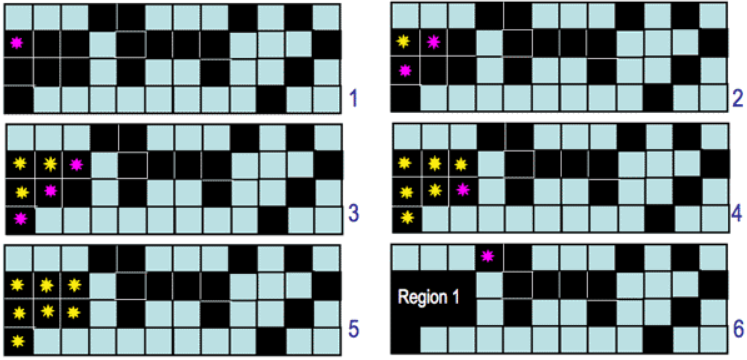
\includegraphics[height=5.5cm]{region_growing_simple_grid.png}
    \caption{ Region growing aiming to label the black object on the top left. The current seed points are fuchsia and the points labelled as ``object'' are yellow. The search algorithm is BFS and pixels are in 4 neighbourhoods.} 
    % src for fig: https://www.cs.auckland.ac.nz/courses/compsci773s1c/lectures/ImageProcessing-html/topic3.htm
\end{figure}



\subsubsection{Region growing implementation from scratch}

\marginnote{\faCogs \ref{app:region_growing_src} \faCogs} As mentioned before, in this article the segmentation is considered complete when all pixels have been assigned a label. This is what the Python program in \ref{app:region_growing_src} does by using BFS. \\ The predicate condition is threshold-based therefore expects an input image and a threshold from the user.

\begin{minipage}{\linewidth}
\captionof{table}{Results of algorithm in App. \ref{app:region_growing_src}.} \label{tab:seed_region_growing_results} 
\begin{center}
\begin{tabular}{| m{.41\textwidth} | m{.15\textwidth} | m{.41\textwidth} |}
\hline   
% image, rank, output, n required, norm 2 of difference, Singular value of rank r+1
    \textbf{Original}  & \textbf{Threshold} & \textbf{Segmented (and replaced by mean)}  \\
\hline 
\hline
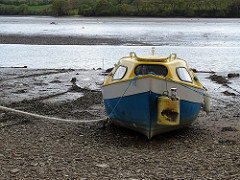
\includegraphics[height=3cm] {sample_06_small.jpg}  &
10 &
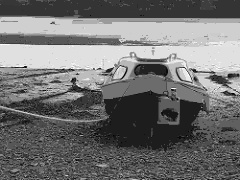
\includegraphics[height=3cm] {sample_06_out.jpg}\\
\hline
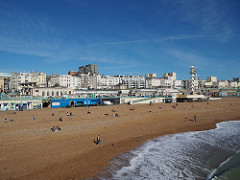
\includegraphics[height=3cm] {sample_07_small.jpg}  &
10 &
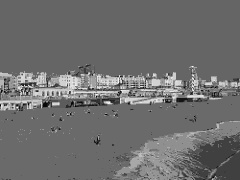
\includegraphics[height=3cm] {sample_07out.jpg}\\
\hline
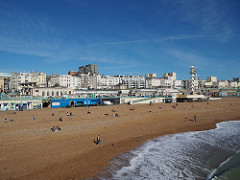
\includegraphics[height=3cm] {sample_07_small.jpg}  &
20 &
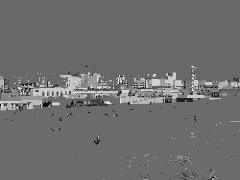
\includegraphics[height=3cm] {sampple_07_out_thr_20.jpg}\\
\hline
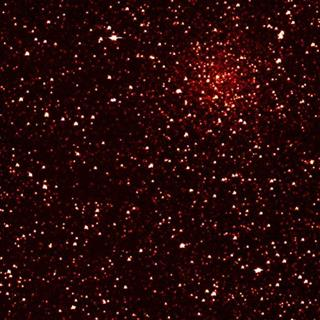
\includegraphics[height=4cm] {sample_03.jpeg}  &
45 &

\includegraphics[height=4cm] {sample_03_out_thr_45.jpeg}\\
\hline

\hline
\end{tabular}
\end{center}
\end{minipage}


\subsubsection{Advantages and pitfalls}
From the table, we can see that seeded region growing can achieve the following objectives.
\begin{itemize}
    \item To produce regions that are as large as possible (i.e., produce as few regions as possible)
    \item To produce coherent regions, but allow some flexibility for variation within the region.
\end{itemize}
However, it can result in oversegmentation if the threshold is too low or in undersegmentation if it is too high. In general, the advantages and disadvantages are:
\begin{multicols}{2}
\begin{itemize}
    \item[\textcolor{DarkPink}{\ding{51}}] Region growing methods can correctly separate the regions that have the same properties we define.
    \item[\textcolor{DarkPink}{\ding{51}}] It is guaranteed (by definition) to produce coherent regions. Linking edges, gaps produced by missing edge is not an issue. It is less susceptible to noise than edge-based methods.
    \item[\textcolor{DarkPink}{\ding{51}}] We can determine the seed point and the criteria we want to make.
\end{itemize}
\columnbreak
\begin{itemize}
    \item[\textcolor{DarkPink}{\ding{55}}] Decisions about region membership are often more difficult than applying edge detector.
    \item[\textcolor{DarkPink}{\ding{55}}] It can't find objects that span multiple disconnected regions. (Whereas edge-based method can be designed to handle “gaps” produced by occlusion—the Hough transform is one example.)
    \item[\textcolor{DarkPink}{\ding{55}}] Heuristics needed, e.g. merging rules and depending on the choice of homogeneity condition and intensity variation, it can easily lead to over or under segmentation as shown in Table \ref{tab:seed_region_growing_results}.
\end{itemize}
\end{multicols}



\subsection{Connected Component labelling using the Hoshen–Kopelman algorithm)}

\subsubsection{Connected components in binary images}
In a binary image, the white pixels are considered as \textit{foreground} and the black and \textit{background}. The goal is to find and label all connected (either 4 or 8-connected) components (CC's) of white pixels and label them, i.e. assign each CC a different integer.\\
Although a seed growing approach could also find the CC's, this one is simpler to implement and doesn't require recursion. Recursion slows down languages that do not support \textit{tail recursion} such as Python, making the approach in the previous section inefficient for large matrices. The algorithm presented below is both relatively fast and memory efficient thanks to the data structure it uses.

\subsubsection{Hoshen–Kopelman intuition}

The Hoshen–Kopelman (H-K) algorithm, or \emphasis{two-pass connected component} operates on a binary image, is simple and relatively efficient as it completes in two \emphasis{raster scans} of the input image. \\
Raster scan divides the image in horizontal, one pixel tall, lines. The image is swept by a window from top left to bottom right line by line.\\
\begin{figure}[H]
    % ref https://www.researchgate.net/figure/Schematic-diagram-of-a-raster-scan-The-electron-beam-scans-later-pixels-in-the-lower_fig1_41823849
    \centering
    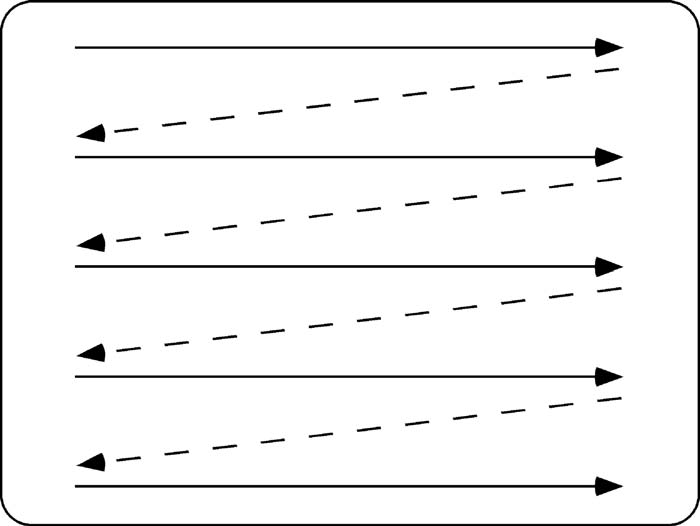
\includegraphics[height=3.4cm]{cc/schematic_raster_scan.png}
    \caption{Raster scan order.}
\end{figure}
As mentioned before, the algorithm performs two scans. Assuming 4-neighbourhood, it is enough to examine only the West and North neighbours of the current pixel. We use 0 for background pixels and 1 for foreground. 

\begin{enumerate}
%ref http://www.mi.auckland.ac.nz/DATA/CCV/books/KR/pdf-LectureNotes/03slides.pdf, http://cs.haifa.ac.il/hagit/courses/ip/Lectures/Ip13_Binary.pdf
    \item On the \textit{first pass} (raster scan), for every pixel P of value 1 (an object pixel), test top and left
neighbours. Background pixels are ingnored.
    \begin{itemize}
        \item If 2 of the neighbours equals 0: assign a new label to P.
        \item If only 1 of the neighbour equals 1: assign the neighbour's label to P.
        \item If 2 of the neighbour equal 1: assign the \textit{smallest} neighbour's label to P. and note equivalence between 2 neighbour’s marks.
    \end{itemize}
    \item Iterate through each element of the data by column, then by row
If the element is not the background
Relabel the element with the lowest equivalent label
assign that label to $p$, and continue the scan.
\end{enumerate}
Before we proceed to the pseudocode, the Figures below visualise the produce.
% ref http://ddeville.me/static/media/research/ucl_report.pdf
\begin{figure}[H]
    \centering
    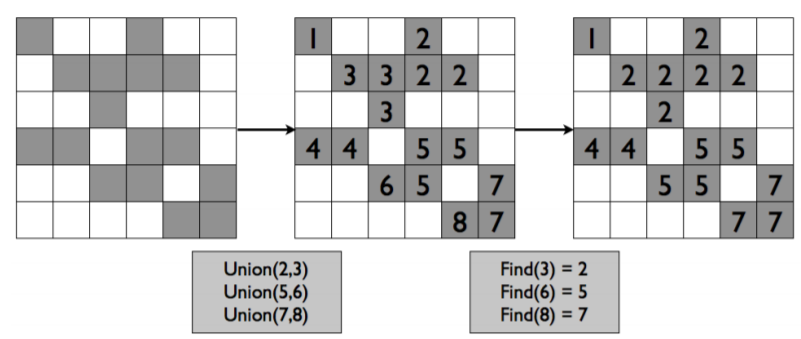
\includegraphics[scale=0.6]{cc/hoshen_on_grid.PNG}
    \caption{The two passes of Hoshen-Kopelman algorithm. Assigning labels and writing equivalencies to the structure (1) and combining equivalent elements (2) using the Union Find structure.}
    %\label{fig:my_label}
\end{figure}


\subsubsection{The Union-Find data structure}
% ref http://cgi.di.uoa.gr/~k08/slides/12-Data-Structures-for-Disjoint-Sets.pdf
The Union-Find structure (aka disjoint set) maintains a collection $S = \{S_1, S_2,\ldots, S_n \}$ of disjoint dynamic sets, i.e. the number of elements in each set can change - they can even get empty. Each set is identified by a \textit{representative}, which is some member of the set and shouldn't change over time.\\
The structure that keeps track of the equivalencies and performs the re-labelling is called \emphasis{union-find}. It can be represented by a tree and its most important feature for our application is \emphasis{path compression}, i.e. all children that lead up to the same parent can drop their hierarchy and point directly to the root (representative). Its representation conforms to the following rules.
\begin{itemize}
    % ref https://www.cs.princeton.edu/courses/archive/spring13/cos423/lectures/UnionFind.pdf
    \item Each element has a parent pointer in the tree.
    \item The root serves as the canonical element.
    \item Each node stores a value, its depth in the tree and a pointer to its parent.
    \item Method FIND(x), where x is a value finds the root of the tree containing x.
    \item Method UNION(x, y), where x, y are some values belonging to different sets makes the root of one tree point to root of other tree.
\end{itemize}
\begin{figure}[H]
    % ref: http://cgi.di.uoa.gr/~k08/slides/12-Data-Structures-for-Disjoint-Sets.pdf
    \centering
    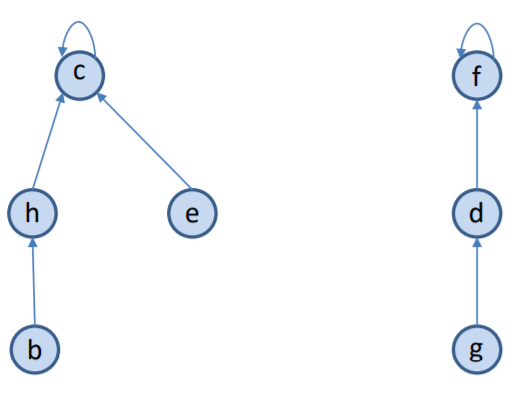
\includegraphics[height=4cm]{img/cc/union_find_tree.PNG}
    \caption{Tree representation of the Sets $S_1 = \{c,h,e,b\}$ and $S_2=\{f,d,g\}$ assuming the representative of $S_1$ is $c$ and of $S_2$ $f$.}
\end{figure}

If $S$ is the universal set, Union-Find for CC labelling must support at least the following operations.
\begin{itemize}
    \item MAKE-SET(x): make a new set $S_i = \{x\}$, and add $S_i$ to $S$.
    % union rank ref: http://granite.sru.edu/~whit/cpsc478/Ch21.pdf
    \item UNION-BY-RANK(x,y): make the root of the smaller tree (fewer nodes) a child of the
root of the larger tree.
    \begin{itemize}
        \item Don't actually use size of tree (number of elements).
        % ref single node rank: http://www.cs.nthu.edu.tw/~wkhon/algo08-lectures/lecture21.pdf
        \item Use \emphasis{rank}, which is an upper bound on height of node. In a single-node tree (created by Make-Set), $rank(root)=0$.
        \item Implemented by making the root with the smaller rank into a child of the root with the larger rank.
    \end{itemize}
    % ref find-set https://www.ics.uci.edu/~goodrich/teach/cs260P/notes/UnionFind.pdf
    \item FIND-SET($x$) returns a pointer to the representative (tree root) of the unique set containing value $x$ and it can be implemented by follow setname pointers from the starting node until reaching a node whose set-name pointer refers back to itself.
    % ref path compr: https://www.cs.princeton.edu/courses/archive/spring13/cos423/lectures/UnionFind.pdf
    \item PATH-COMPRESSION(x): After finding the root r of the tree containing x, change the parent pointer of all nodes along the path to point directly to r. This implies a fast "almost linear" time $\mathcal{O}(n)$ for $n$ union-find operations.
\end{itemize}
\begin{figure}[H]
    % ref http://cgi.di.uoa.gr/~k08/slides/12-Data-Structures-for-Disjoint-Sets.pdf
    \centering
    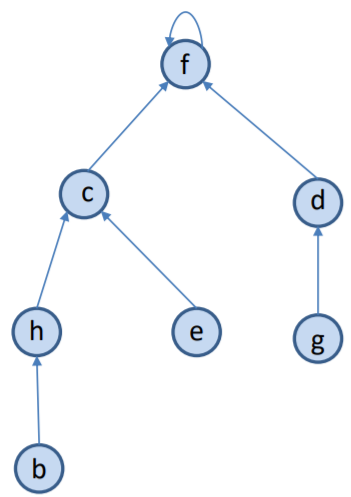
\includegraphics[height=3.5cm]{cc/union_by_rank2.PNG}
    \caption{Result of union by rank on sets $\{c,h,e,b\}$ and $\{f,d,g\}$.}
\end{figure}
\TODO[path compression figs]
The pseudocode for the basic methods described would be as follows. The value attribute of each node is omitted for simplicity.

%ref https://www.cs.princeton.edu/courses/archive/spring13/cos423/lectures/UnionFind.pdf

\begin{algorithm}[H]
\caption{Make-set method.}
\begin{algorithmic}[1]
\Procedure{Make-Set}{$x$}
    \State $parent(x) \leftarrow x$
    \State $rank(x) \leftarrow 0$ 
\EndProcedure
\end{algorithmic}
\end{algorithm}

\begin{algorithm}[H]
\caption{Find method.}
\begin{algorithmic}[1]
\Procedure{Find}{$x$}
    \While{$x\neq parent(x)$}
    \State $x \leftarrow parent(x)$
    \EndWhile
\State \textbf{return} $x$
\EndProcedure
\end{algorithmic}
\end{algorithm}

\begin{algorithm}[H]
\caption{Union by rank method.}
\begin{algorithmic}[1]
\Procedure{Union-By-Rank}{$x,y$}
    \State $r \leftarrow FIND (x)$
    \State $s \leftarrow FIND(y)$
    \If {$r == s$}
      \State \textbf{return}  
    \ElsIf{$rank(r) > rank(s)$}
        \State $parent(s) \leftarrow r$
    \ElsIf{$rank(r) < rank(s)$}
        \State $parent(r) \leftarrow s$
    \Else{}
        \State $parent(r) \leftarrow s$
        \State $rank(s)++$
    \EndIf
\EndProcedure
\end{algorithmic}
\end{algorithm}

%%%%%%%%%%%%% path - compress
%FIND-SET(��)
% if �� ≠ p[��]
% then p[��] ← FIND-SET(p[��])
% return p[��]







\subsubsection{Hoshen-Kopelman algorithm and implementation}

The pseudocode summarising the procedure would be as follows. \TODO[UF structure]
\begin{algorithm}[H]
\caption{Region labelling for a single seed}\label{alg:region_growing_one_seed}
\begin{algorithmic}[1]
\Procedure{Hoshen-Kopelman}{$P_{m\times n}$} \Comment{P for pixels...}
% ref https://www.ocf.berkeley.edu/~fricke/projects/hoshenkopelman/hoshenkopelman.html, http://ddeville.me/static/media/research/ucl_report.pdf
\State $label \leftarrow \textbf{0}_{m \times n}$
\State $largestLabel\leftarrow 0$
\State $UF \leftarrow \{\}$ \Comment{Initialise union find structure.}
\For{x \ in \ $0 \, \ldots \, m$ }
    \For{y \ in \ $0 \, \ldots \, n$ }
        \If {$P[x,y] \neq 0$}
            \State $pLeft \leftarrow P[x-1,y]$
            \State $pAbove \leftarrow P[x,y-1]$
            
            \If{ $pLeft = 0$ and $pAbove = 0$}
                \State $largestLabel++ $ \Comment{Neither neighbour is foreground}
                \State $label[x,y] \leftarrow largestLabel$ \Comment{Make a new, as-yet-unused cluster label.}            
            \ElsIf {$pLeft \neq 0 \quad and \quad pAbove = 0$} \Comment{Only one neighbour, left.}
                \State \textbf{let} $label[x,y] \leftarrow label[x,y-1]$ \Comment{Look left.}
            \ElsIf {$pLeft = 0 \quad and \quad pAbove \neq 0 $} \Comment{Only one neighbour, above.}
                \State $label[x,y] \leftarrow label[x-1,y]$ \Comment{Look up.}
            
            \Else {} \Comment{Both neighbours are foreground (and have been labelled).}
                \State $lblLeft \leftarrow lbl[x,y-1]$
                \State $lblAbove \leftarrow lbl[x-1,y]$
                \State UF.union(lblLeft, lblAbove) \Comment{Link left and above clusters.}
                \State $label[x,y] \leftarrow \min(lblLeft,\, lblAbove)$
            \EndIf
        \EndIf
    \EndFor
\EndFor
\State
\For{x in $0 \, \ldots \, m$ }
    \For{y in $0 \, \ldots \, n$ }
        \If {$P[x,y] \neq 0$}
            \State $label[x,y] \leftarrow UF.find\left(label[x,y]\right)$ \Comment{Replace with corresponding parent.}
        \EndIf
    \EndFor
\EndFor
\State \textbf{return} label
\EndProcedure
\end{algorithmic}
\end{algorithm}
\marginnote{\faCogs\ref{app:hk_algo_source}\faCogs}H-K algorithm has also been written in Python in \ref{app:hk_algo_source}. To run, except of OpenCV and Numpy, package \mintinline{Python}{python_algorithms} needs to be installed, e.g. using \mintinline{Python}{pip} from the command line:
\begin{minted}{python}
pip install python_algorithms
\end{minted}
The Union-Find structure can be imported by:
\begin{minted}{latex}
from python_algorithms.basic.union_find import UF
\end{minted}
More details in the documentation.



% diagram from https://www.youtube.com/watch?v=ticZclUYy88 


% uf:
% https://courses.cs.washington.edu/courses/cse326/09wi/lectures/19-disjoint-union-find-part-2.pdf
% https://www.techiedelight.com/disjoint-set-data-structure-union-find-algorithm/
%https://sarielhp.org/teach/2004/b/webpage/lec/22_uf.pdf, https://courses.cs.washington.edu/courses/cse373/17wi/lectures/union-find.pdf, https://dev.to/bobfang1992/a-short-summary-of-the-union-find-algorithm
% http://staff.ustc.edu.cn/~csli/graduate/algorithms/book6/chap22.htm

% pseudo : http://hpcg.purdue.edu/papers/Stava2011CCL.pdf



% sources:
% http://cs.haifa.ac.il/hagit/courses/ip/Lectures/Ip13_Binary.pdf
% http://aishack.in/tutorials/labelling-connected-components-example/
% https://jacklj.github.io/ccl/
% http://www.mi.auckland.ac.nz/DATA/CCV/books/KR/pdf-LectureNotes/03slides.pdf
% http://hpcg.purdue.edu/papers/Stava2011CCL.pdf
% https://www.youtube.com/watch?v=ticZclUYy88
% http://service.hidebux.com/index.php?q=n9XX1Z9gZ8-YpZqd0WSm296XyKmYw5GZpNJfYZOccp1tkpiT1ZWe http://marcin.szyderca.com/00797615.pdf
% union find: https://web.archive.org/web/20170712162245/https://www.ida.liu.se/opendsa/OpenDSA/Books/Everything/html/UnionFind.html
% union find https://www.cs.princeton.edu/courses/archive/spring13/cos423/lectures/UnionFind.pdf
% https://dsp.stackexchange.com/questions/10531/connected-component-labeling-equivalence-table
% overview https://en.wikipedia.org/wiki/Connected-component_labeling
% https://www.ocf.berkeley.edu/~fricke/projects/hoshenkopelman/hoshenkopelman.html
% http://web.eecs.utk.edu/~mberry/aldridge/slides.pdf

% http://cs.haifa.ac.il/hagit/courses/ip/Lectures/Ip13_Binary.pdf
% http://aishack.in/tutorials/labelling-connected-components-example/
% http://www.mi.auckland.ac.nz/DATA/CCV/books/KR/pdf-LectureNotes/03slides.pdf
% http://hpcg.purdue.edu/papers/Stava2011CCL.pdf
% https://www.cs.princeton.edu/courses/archive/spring13/cos423/lectures/UnionFind.pdf

% UF
% https://web.archive.org/web/20170712162245/https://www.ida.liu.se/opendsa/OpenDSA/Books/Everything/html/UnionFind.html
% https://python-algorithms.readthedocs.io/en/stable/_modules/python_algorithms/basic/union_find.html
% https://www.youtube.com/watch?v=0jNmHPfA_yE
% http://www14.in.tum.de/lehre/2015WS/ea/split/sec-Union-Find-handout.pdf
% http://www.cs.tau.ac.il/~zwick/Data-Structures-2013/Union-Find.pdf
% http://tuvalu.santafe.edu/~aaronc/courses/5454/csci5454_spring2013_CSL1.pdf
% https://web.archive.org/web/20170712162245/https://www.ida.liu.se/opendsa/OpenDSA/Books/Everything/html/UnionFind.html
% http://www.cs.toronto.edu/~krueger/cscb63h/lectures/tut07.txt
% https://algs4.cs.princeton.edu/15uf/
% https://ocw.mit.edu/courses/electrical-engineering-and-computer-science/6-046j-design-and-analysis-of-algorithms-spring-2012/lecture-notes/MIT6_046JS12_lec16.pdf


\subsubsection{A case study on huh7 cells; connected components for label information extraction}

Hoshen-Kopelman ideal for labelling components in binary images. However, when we have a labelled image, i.e. each CC has a different intensity H-K can also be used to extract information about each CC, such as its centre of mass.\\
% ref http://www.cs.bilkent.edu.tr/~gunduz/downloads/NucleusSegData/
H-K was used as part of the workflow to locate Huh7 cells from a dataset from Bilkent University. Huh7 cells are generally ellipsoid in shape and often largely overlap each other, which poses a challenge when detecting/ locating them. This is the workflow followed to detect them and where H-K comes in handy.

\begin{enumerate}
    \item Extract foreground from RGB image by converting it to the HSV domain and then to black and white.
    \item Perform \textit{progressive top hat transform} (top hat transform is a morphological operation described in \ref{app:morphology}) with growing disks and the structuring element. The minimum radius of the disk is the minimum cell radius we want to detect and similarly for the maximum. At each step, the top-hat outputs a BW image. Circular objects that have the same radius as the structuring element end up white. Thus, two overlapping cells will not be detected in the same step of the top-hat. In the end, all outputs of the top-hat are accumulated into one greyscale image where different intensity implies different CC.
    \item H-K can be used to look for areas with constant intensity and assign them a label (a unique integer to each).
\end{enumerate}
The code in \ref{app:cc_huh7} implements labelling both using H-K and using \mintinline{python}{scikit} library's functionality. The drawback of the current implementation is taht is only considers 4-neighbours, so \mintinline{python}{scikit} performs slightly better.
\begin{multicols}{2}
\begin{figure}[H]
    \centering
    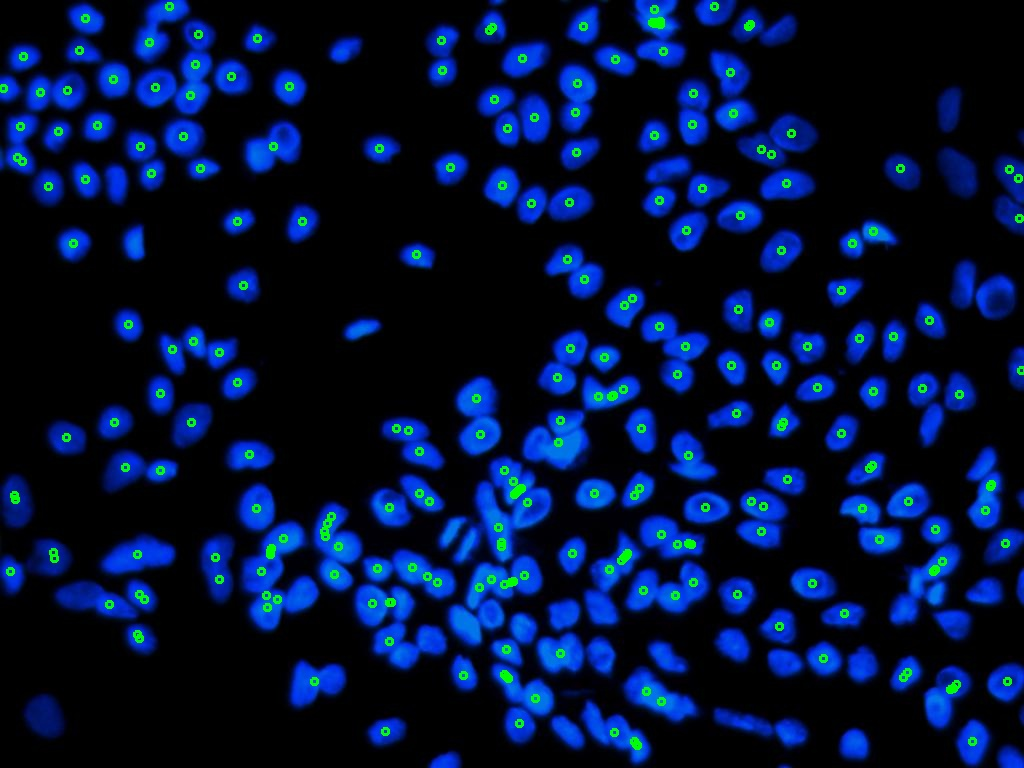
\includegraphics[height=4cm]{img/cc/huh7_test11_man.jpg}
    \caption{Labelling result for a huh7 cell image 11 using the manual approach (H-K) for \mintinline{python}{min_size=12, max_size=48, step=4} (see \ref{app:cc_huh7}). Detected cells in greens.}
    %\label{fig:my_label}
\end{figure}
\columnbreak
\begin{figure}[H]
    \centering
    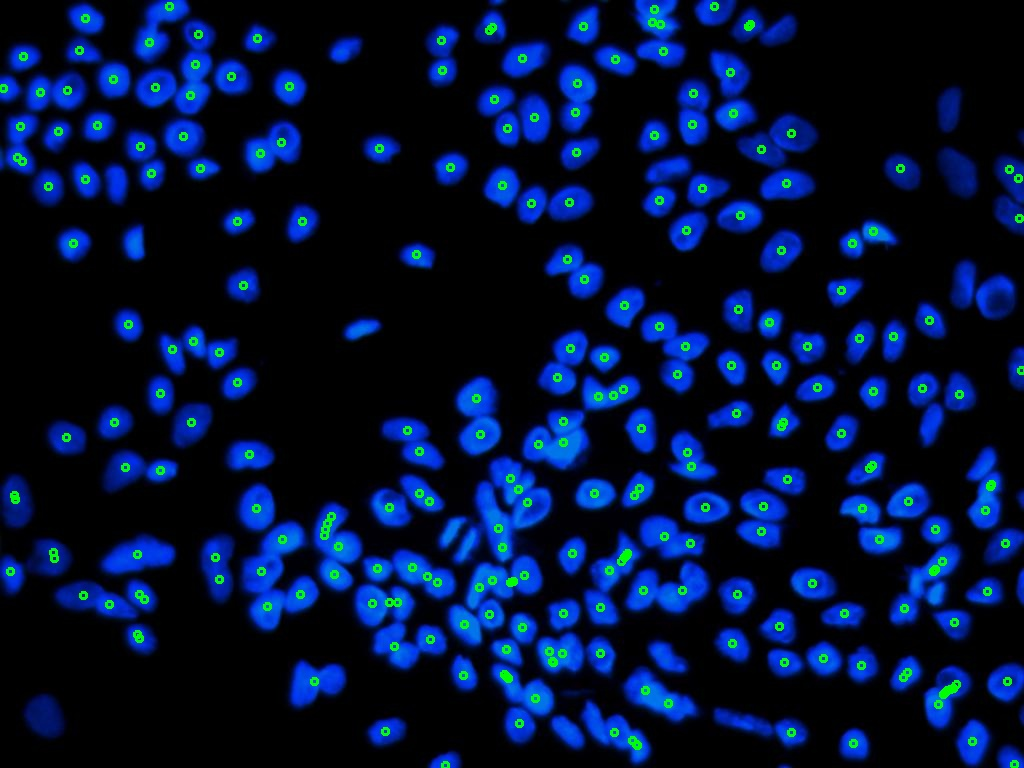
\includegraphics[height=4cm]{img/cc/huh7_test11_sci.jpg}
    \caption{Labelling result for a huh7 cell image using the scikit's.}
    %\label{fig:my_label}
\end{figure}
\end{multicols}





\subsection{Split and Merge Approach}


% split merge bst http://www.intelligence.tuc.gr/~petrakis/courses/computervision/advancedsegmentation.pdf
% good split merge https://nptel.ac.in/courses/117105135/59
% split merge http://disp.ee.ntu.edu.tw/meeting/%E6%98%B1%E7%BF%94/Segmentation%20tutorial.pdf
% splt merge http://web.cecs.pdx.edu/~mperkows/CLASS_479/S2006/13-region.pdf
% spit merge paper https://www2.cs.duke.edu/courses/spring06/cps296.1/handouts/Horowitz%20Pavlidis%201976.pdf
% sp me https://stackoverflow.com/questions/7050164/image-segmentation-split-and-merge-quadtrees
% s m http://user.engineering.uiowa.edu/~dip/lecture/segmentation3.html
% sm https://de.mathworks.com/matlabcentral/fileexchange/25619-image-segmentation-using-statistical-region-merging
% s m http://homepages.inf.ed.ac.uk/rbf/CVonline/LOCAL_COPIES/MARBLE/medium/segment/split.htm
% http://www.cse.usf.edu/~r1k/MachineVisionBook/MachineVision.files/MachineVision_Chapter3.pdf
% https://www.uni-koblenz.de/~lb/lb_activities/ipcv02/download/lectures.pdf
% https://www.uni-koblenz.de/~lb/lb_activities/ipcv02/download/lectures.pdf
% https://de.mathworks.com/help/images/ref/qtdecomp.html




\emphasis{Split and merge} is a \emphasis{top-bottom} approach and attempts to divide an image into uniform regions. This process starts by examining the whole image and is then repeated on each of the sub-regions until no further splitting is necessary, i.e. until each sub-region is considered homogeneous. \\
Splitting always happens in a characteristic way, that is, when $P(R_i)=False$ for a region $R_i$, it is split in 4 \emphasis{quadrants} $R_{i1}, R_{i2}, R_{i3}, R_{i4}$. This, however, often results in in too many segmented regions. After the initial intensity-based region segmentation, the regions may need to be refined or reformed. \\
The \emphasis{merge operation} combines neighbouring regions that are considered similar. In this implementation, the uniform criterion for splitting is the \emphasis{standard deviation} threshold, i.e. if for a region $R_i$ $\sigma_{i} < \sigma$, where $\sigma$ is fixed for the whole image, then we stop splitting $R_i$. The merge critetion is the \emphasis{mean}, i.e. if the means of two neighbouring regions $R_i, R_j$ are close enough then they are merged; $\left|\mu_i - \mu_j \right| < \mu$. So split and merge takes a split threshold and a merge threshold as parameters.\\
A very loose high-level view of the algorithm is below.
\begin{verbatim}
Let PS be the predicate splitting condition and MS the merge condition.
Initialise a structure to store segments
:Splitting step
For any region Ri do
    In case Ri is not homogeneous, i.e. SM(Ri) == False
        then split Ri in 4 and repeat Splitting step
    else
        store Ri in structure
        split next region
:Merge step
When no further splitting is possible, merge any adjacent segments for which MS is true.
\end{verbatim}

The data structure that performs the splitting is the \emphasis{quadtree}, discussed below.




\subsubsection{The quad tree structure}

\emphasis{Quadtree} is a rooted tree in which every node has 4 children that has the following properties:
\begin{itemize}
    \item The root of the tree encompasses the region of interest (e.g. stores the whole image). The region of interest must be a square.
    \item Each node corresponds to a square in the plane.
    \item Each node stores a region of the original image.
    \item Each node has 4 children nodes and child corresponds to a quadrant of the parent node.
    \item A quadtree induces a subdivision of the image stored in the root.
\end{itemize}
The \emphasis{root} of the tree stores the whole image, i.e. the least detailed features and the \emphasis{leaves} store the finest level of detail possible. The union of the images stored in all leaves yields the original image.\\
When the image region $R_i$ stored in a node is not homogeneous enough, i.e. satisfied the predicate condition, the the node recusrively splits in four children. An example of splitting and merging using that structure is visualised below.

\begin{multicols}{2}
\begin{figure}[H]
    \label{alg:split_merge_high}
	\centering %centralizar a figura
	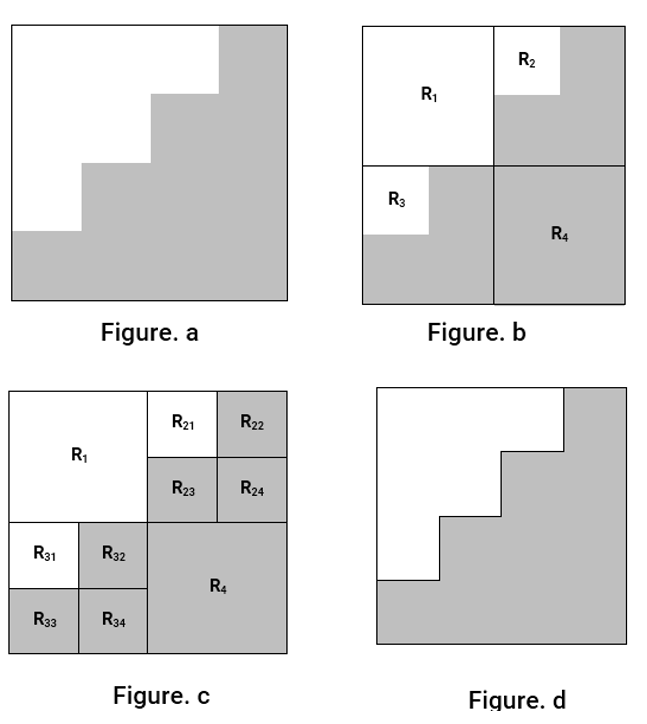
\includegraphics[height=4.5cm]{image_splitting_merging.png}
    \caption{ (a) The original 1 bpp image as a region $R$ (b) $R$ is not homogeneous so it is split in 4 (c) $R_1$ and $R_4$ are homogeneous and $R_2$, $R_3$ are not so they are split in 4 (d) The outcome of the merging step} 
    % src http://www.ques10.com/p/29865/segment-the-following-image-using-region-split-and/
\end{figure}
\columnbreak
\begin{figure}[H]
	\centering %centralizar a figura
	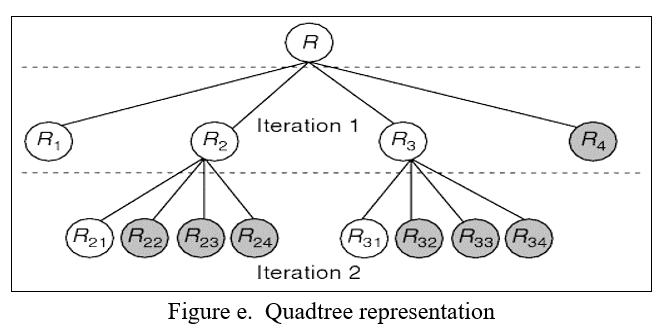
\includegraphics[height=4.5cm]{image_quadtree_example.png}
    \caption{ The corresponding quadtree for each step. Each node stores a region of the image} 
    % src http://www.ques10.com/p/29865/segment-the-following-image-using-region-split-and/
\end{figure}
\end{multicols}

A quadtree implementation in Python is listed in \ref{app:app_quadtree}. \marginnote{\faCogs \ref{app:app_quadtree} \faCogs} Some of the results of that code are presented in the table below. To clarify the merge step of Alg. \ref{alg:split_merge_high}, it could e.g. consist of comparing the mean intensity of two adjacent regions to a threshold.

\begin{minipage}{\linewidth}
\captionof{table}{Results of the quadtree splitting in \ref{app:app_quadtree}.} \label{tab:quad_tree_results} 
\begin{center}
\begin{tabular}{| m{.41\textwidth} | m{.15\textwidth} | m{.41\textwidth} |}
\hline   
% image, rank, output, n required, norm 2 of difference, Singular value of rank r+1
    \textbf{Original}  & \textbf{Threshold} & \textbf{Segmented (and replaced by mean)}  \\
\hline 
\hline
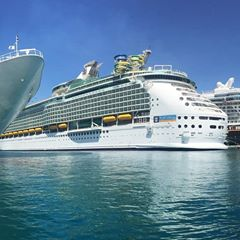
\includegraphics[height=3cm] {segm_split_merge/ship_240x240.jpg}  &
10 &
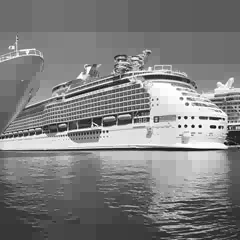
\includegraphics[height=3cm] {segm_split_merge/output_thr_10.png}\\
\hline
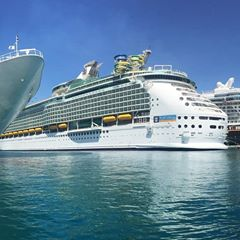
\includegraphics[height=3cm] {segm_split_merge/ship_240x240.jpg}  &
25 &
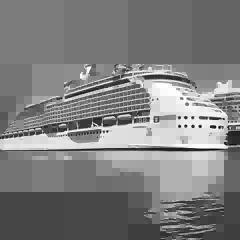
\includegraphics[height=3cm] {segm_split_merge/output_thr_25.png}\\
\hline
\end{tabular}
\end{center}
\end{minipage}
The lower the splitting theshold, the higher the oversegmentation and a similar statement can be made for the undersegmentation.





\subsubsection{The merge phase}

In the merge phase, neighbouring quadtrants with similar characteristics (merge condition) are merged into one segment in a procedure described by the algorithm below.
% ref https://www.uni-koblenz.de/~lb/lb_activities/ipcv02/download/lectures.pdf
\begin{algorithm}[H]
\caption{Quadrant merging}\label{alg:region_quadrant_merging}
\begin{algorithmic}[1]
\Procedure{merge}{$T$} \Comment{$T$ is the generated quadtree}
\State $S \gets \textup\{\}$ \Comment{empty set of quadtrees}
\For {all leaves $L$ of $T$}
\State \textbf{append} to $S$ a new quadtree with $L$ as root and only leaf
\EndFor
\For {\textbf{any} root $L$ in $S$}
\For {any other root $L'$ in $S$}
\If {merging condition is \textbf{True} for $L$ and $L'$} \Comment{condition: neighbours and similar}
\State \textbf{create} a new root $\hat{L}$ in $S$ with children $L,L'$
\State \textbf{store} the segment $R_L \cup R_{L'}$ in $\hat{L}$
\EndIf
\EndFor
\EndFor
\EndProcedure
\end{algorithmic}
\end{algorithm}
% algo src: https://www.uni-koblenz.de/~lb/lb_activities/ipcv02/download/lectures.pdf



%example of quad tree:
% \url{http://www.ques10.com/p/29865/segment-the-following-image-using-region-split-and/} \\
% \url{https://gamedevelopment.tutsplus.com/tutorials/quick-tip-use-quadtrees-to-detect-likely-collisions-in-2d-space--gamedev-374} \\
% \url{http://personal.us.es/almar/cg/09quadtrees.pdf} \\
% \url{http://www.bowdoin.edu/~ltoma/teaching/cs350/fall14/Lectures/gis_qdt.pdf}\\
% \url{https://kpully.github.io/Quadtrees/} \\
% \url{http://www.fundza.com/algorithmic/quadtree/index.html} \\
% \url{http://www.cs.unca.edu/~reiser/imaging/quadtree.html} \\

The lower the splitting threshold, the more the (blocky) oversegmentation and a similar statement can be made for the (blocky) undersegmentation. The problem with quad splitting is that adjacent regions could have similar properties, so merging is required.


%example of quad tree:
% \url{http://www.ques10.com/p/29865/segment-the-following-image-using-region-split-and/} \\
% \url{https://gamedevelopment.tutsplus.com/tutorials/quick-tip-use-quadtrees-to-detect-likely-collisions-in-2d-space--gamedev-374} \\
% \url{http://personal.us.es/almar/cg/09quadtrees.pdf} \\
% \url{http://www.bowdoin.edu/~ltoma/teaching/cs350/fall14/Lectures/gis_qdt.pdf}\\
% \url{https://kpully.github.io/Quadtrees/} \\
% \url{http://www.fundza.com/algorithmic/quadtree/index.html} \\
% \url{http://www.cs.unca.edu/~reiser/imaging/quadtree.html} \\

Some results of the whole algorithm are presented below.
% src:http://homepages.inf.ed.ac.uk/rbf/CVonline/LOCAL_COPIES/MARBLE/medium/segment/split.htm

\begin{multicols}{2}
\begin{figure}[H]
	\centering %centralizar a figura
	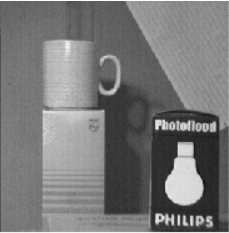
\includegraphics[height=3.25cm]{split_merge_result1.PNG}
    \caption{Input greyscale image.} 
    % src http://www.ques10.com/p/29865/segment-the-following-image-using-region-split-and/
\end{figure}
\columnbreak
\begin{figure}[H]
	\centering %centralizar a figura
	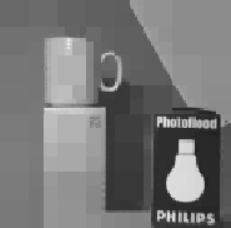
\includegraphics[height=3.25cm]{split_merge_result2.PNG}
    \caption{After quad splitting.} 
    % src http://www.ques10.com/p/29865/segment-the-following-image-using-region-split-and/
\end{figure}
\end{multicols}

\begin{figure}[H]
	\centering %centralizar a figura
	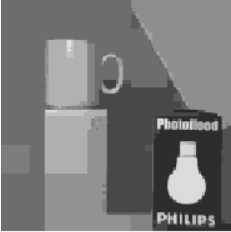
\includegraphics[height=3.25cm]{split_merge_result3.PNG}
    \caption{After merging.} 
    % src http://www.ques10.com/p/29865/segment-the-following-image-using-region-split-and/
\end{figure}
To summarise the split and merge segmentation.
\begin{multicols}{2}
Advantages:
\begin{itemize}
    \item[\textcolor{DarkPink}{\ding{51}}] The image could be split progressively according to our demanded resolution because the number of splitting level is determined by us.
    \item[\textcolor{DarkPink}{\ding{51}}]  We could split the image using the criteria we decide, such as mean or variance of segment pixel value. In addition, the merging criteria could be different to the splitting criteria. 
    \item[\textcolor{DarkPink}{\ding{51}}] Seed points are not needed but predicate conditions are, so less heuristics than seed-based growing.
\end{itemize}
\columnbreak
Disadvantages:
\begin{itemize}
    \item[\textcolor{DarkPink}{\ding{55}}]  It may produce the "blocky" segments. The blocky segment problem could be reduced by splitting in higher level, but the trade off is that the computation time will increase.
\end{itemize}
\end{multicols}






\subsection{Active contours and snakes} 


\subsubsection{Definitions and Snake Energies}
% ref: https://www.cise.ufl.edu/class/cap5416fa18/slides2017/Snakes_GVF.pdf
Active contours are elastically deformable curves (can be throught as elastic bands)
whose behaviour is based on elasticity theory. They can
deform under externally applied forces and come to
rest under force balance. Active contours are
represented using a parametric curves. 
The parametric curve is assigned an
\emphasis{internal energy} and \emphasis{external energy}.
The problem of segmenting an object
boundary is cast in an energy
minimisation framework.\\
A higher level, a process or a user initialszes the snake
close to the object boundary to be segmented.
The snake then starts deforming and in an iterative manner moving towards
the desired object boundary.
In the end, it sticks to the object boundary or “shrink
wraps” the object boundary for closed boundaries

\begin{figure}[H]
	\centering %centralizar a figura
    	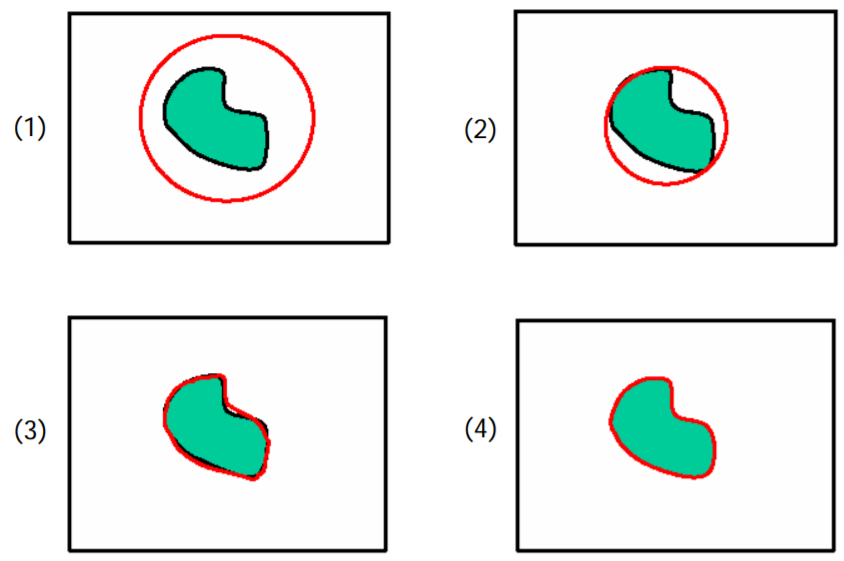
\includegraphics[width=4.5cm]{snakes/demo_snake_sample_object.PNG}
    \caption{Synthetic example of snake around an object. In the initialisation, the snake encloses the object and at every iteration it shrink wraps around it.}
\end{figure}


\begin{definition}
The contour is defined in the $(x,y)$ plane of an image as a
parametric curve $v(s) = \left(x(s), y(s)\right)$. In the discrete domain, we consider a contour as a set of 2D positions (vectices) $v_i = (x_i,y_i), \ i = 0,1,\ldots, n-1$.
\end{definition}
The curve is usually closed, i.e. $v_0 = v_{n-1}$.
% ref: TP11 - Fitting: Deformable contours Miguel Coimbra
An energy cost function governs the shape of the active contour at each iteration. \begin{itemize}
    \item Keep it near image positions with high gradients.
    \item Satisfy shape ``preferences'' or contour priors.
\end{itemize}. We define it as a sum of energies, each of which encapsulates one of the above criteria.:
\begin{equation}
    E_{total} = E_{int} +E_{ext} + E_{con} 
\end{equation}
\begin{itemize}
% ref https://www.inf.u-szeged.hu/~kato/teaching/emm/02-Snake.pdf
    \item $E_{int}$ is the internal energy due to bending and stretching. Serves to impose = internal energy due to bending. Serves to impose piecewise smoothness constraint.
    \item $E_{ext}$ is the image forces (think of them as gravitational forces) pushing the snake toward image  features  of high contrast (edges, etc.).
    \item $E_{con}$ are the external constraints responsible for putting the snake near the desired local minimum. It may come from higher level interpretation or user interaction.
\end{itemize}


\subsubsection{The external energy - intuition and definition}

As mentioned before, the external energy should be minimised at feature points, therefore given an image $I$ it is conventient to define it in terms of the image gradient $\textbf{G}=(G_x,G_y) = \left(\tfrac{\partial I}{\partial x},\tfrac{\partial I}{\partial y}\right)$.
\begin{multicols}{2}
\begin{figure}[H]
	\centering %centralizar a figura
    	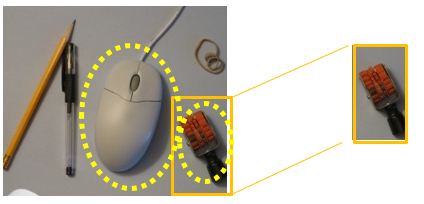
\includegraphics[height=3.00cm]{snakes/example_obj_for_snake.PNG}
    \caption{A sample object in an image.}
\end{figure}
\columnbreak
\begin{figure}[H]
	\centering %centralizar a figura
    	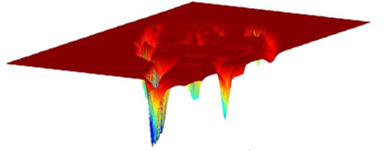
\includegraphics[height=3.00cm]{snakes/example_obj_ext_energy.PNG}
    \caption{Its negated gradient magnitude, i.e. $-\left(G_x^2 + G_y^2 \right)$.}
\end{figure}
\end{multicols}
The lower the gradient magnitude $G_x^2 + G_y^2$, the smaller we want the external energy. Therefore for a single vertice $v$ can be defined as:
\[
    E_{ext}(v) = -\left(G_x^2 + G_y^2 \right)
\]
However this can product extreme values. To regularlise it, we can normalise the gradient norm as follows
% ref http://www.sci.utah.edu/~gerig/CS7960-S2010/project5/snake-Trucco-Verri.pdf
\begin{equation}
    E_{ext}(v) = -\frac{\left| \left| \nabla I(v)  \right| \right| -m}{M-m}
\end{equation}
, where $m,\ M$ are the minimum and maximum respectively of $\nabla I$ over tge currently examined 8-neighbourhood.
\begin{definition}
The external energy for the whole contour is defined as
\begin{equation}
    E_{ext} = -\sum\limits_{i=0}^{n-1}{-\frac{\left| \left| \nabla I(\textbf{v}_i)  \right| \right| -m}{M-m}}
    \label{eq:snake_e_ext}
\end{equation}
\end{definition}


\subsubsection{The internal energy - intuition and definition}

% ref http://www.cs.cornell.edu/courses/cs664/2005fa/Lectures/lecture23.pdf
It depends on the intrinsic properties of the curve and encourages smoothness or any particular shape Internal energy treats the curve as an elastic rubber band possessing  potential energy. It discourages stretching by introducing tension. It minimises:
% ref https://www.cse.wustl.edu/~pless/519/Lecture17.pdf
\begin{itemize}
    \item How far apart the snake points are from one another (the so called \textit{elastic energy}).
    \item How much the curve bends (\textit{bending energy}).
\end{itemize}
Therefore internal energy can be treated as the sum of \emphasis{elastic energy} and \emphasis{bending energy}.

\begin{multicols}{2}
\begin{figure}[H]
	\centering %centralizar a figura
    	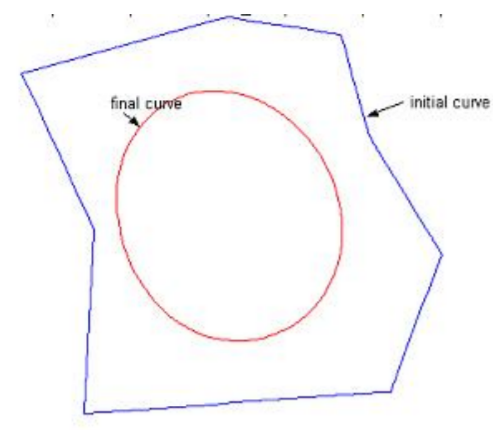
\includegraphics[width=3.25cm]{snakes/action_elastic_energy.PNG}
    \caption{The effect of elestic energy.}
\end{figure}
\columnbreak
\begin{figure}[H]
	\centering %centralizar a figura
    	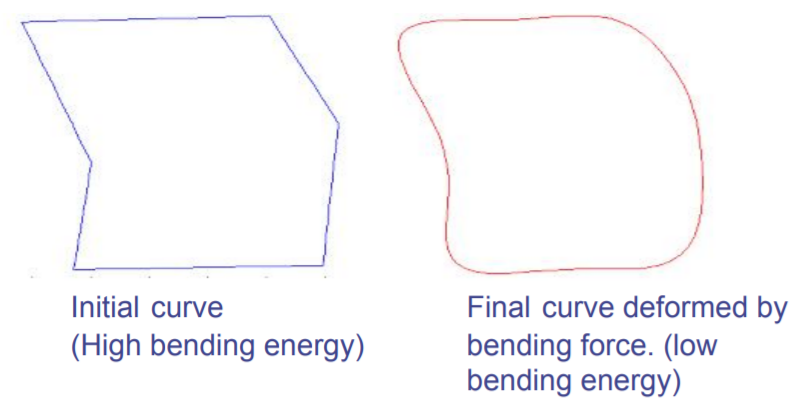
\includegraphics[width=4.5cm]{snakes/action_bending_force.PNG}
    \caption{The effect of bending energy.}
\end{figure}
\end{multicols}


\subsubsection{Elastic Energy ($E_{elastic}$)}
As already, mentioned, elastic energy wants to minimise stretching. Given a continuous curve $v$, at some point $v(s)$ the internal energy can be computed as:
\begin{equation}
    E_{int}\left(v(s) \right) = \alpha \left| \frac{dv}{ds} \right|^2
\end{equation}
As a discrete approximation with $\textbf{v}_i = (x_i,y_i),\ i=0,1,\ldots,n-1$, we have the approximation
\begin{equation}
    E_{int} \approx \alpha \left|\left|\textbf{v}_{i+1} - \textbf{v}_i\right|\right|^2
\end{equation}
Therefore the total \emphasis{elastic energy} of the contour is
\begin{equation*}
    E_{int} = \sum\limits_{i=0}^{n-1}{\alpha \left|\left|\textbf{v}_{i+1} - \textbf{v}_i\right|\right|^2}
\end{equation*}
% ref TP11 - Fitting: Deformable contours FCUP, 20134
However, this definition has the effect of causing the contour to shrink too much. To rectify this and keep distances even we can adjust it as follows.
%ref (def) https://www.dcc.fc.up.pt/~mcoimbra/lectures/VC_1213/VC_1213_T11_KGrauman_ActiveContours.pdf
\begin{definition}
The revised total \emphasis{elastic energy} of the contour is
\begin{equation}
    E_{int} = \sum\limits_{i=0}^{n-1}{ \alpha \left(\left|\left|\textbf{v}_{i+1} - \textbf{v}_i- \right|\right|- \overline{d}_i\right)^2 }
\end{equation}
$\overline{d}_i$ is the average distance between pairs of points – updated at each iteration.
\end{definition}

 
\subsubsection{Bending Energy ($E_{bend}$)}

The purpose of bending energy is to penalise high contour curvatures. Curvature is captured by the second derivative of the continuous curve $v(s)$, i.e. we can define at a point $v(s)$:
\[
E_{bend}\left(v(s)\right) = \beta\left|\frac{d^2v}{ds^2}\right|^2
\]
If we want to transfer to the discrete domain once again at a point $\textbf{v}_i=(x_i,y_i)$, then $\tfrac{d^2v}{ds^2}\approx (v_{i+1} - v_i) - (v_i - v_{i-1}) =v_{i+1} - 2v_i + v_{i-1}$ hence
\[
E_{bend}\left(v(s)\right)=\beta\left|\frac{d^2v}{ds^2}\right|^2=\beta\left| v_{i+1} - 2v_i + v_{i-1} \right|^2
\]
\begin{definition}
The total \emphasis{bending energy} of a curve $v_0, v_1,\ldots, v_{n-1}$ is
\begin{equation}
    E_{bend}=\sum\limits_{i=0}^{n-1} \beta\left| v_{i+1} - 2v_i + v_{i-1} \right|^2
\end{equation}
\end{definition}
\begin{definition}
The total internal energy of a curve $v_0, v_1,\ldots, v_{n-1}$ is
\begin{equation}
    E_{int} = E_{elastic} +  E_{bend}=\sum\limits_{i=0}^{n-1}{\left( \alpha \left(\left|\left|\textbf{v}_{i+1} - \textbf{v}_i \right|\right|- \overline{d}_i\right)^2 +
    \beta\left|\left|  v_{i+1} - 2v_i + v_{i-1} \right|\right|^2 \right)}
    \label{eq:snake_e_int}
\end{equation}
\end{definition}


\subsubsection{Minimising the snake energy}
% ref vieterbi: http://home.netcom.com/~chip.f/viterbi/algrthms2.html
There exist multiple approach to minimise the total energy such as by dynamic programming using the Viterbi algorithm \TODO[ref]. In this report we use the simplest appraoch - the greedy one. We have modelled the total snake energy of the set of points $v_i,\ i=0,\ldots,n-1$ as $E_{total} = E_{int} +E_{ext} + E_{con}$. Setting $E_{con}=0$ as we're currently not interested in it and using \eqref{eq:snake_e_ext}, \eqref{eq:snake_e_int} we derived that
\begin{equation}
    E = \sum\limits_{i=0}^{n-1}{\left( \alpha \left( \left|\left|\textbf{v}_{i+1} - \textbf{v}_i\right|\right| -\overline{d}_i \right)^2 +
    \beta\left|\left|  v_{i+1} - 2v_i + v_{i-1} \right|\right|^2 -
    \gamma  \frac{\left| \left| \nabla I (\textbf{v}_i) \right| \right| -m}{M-m}  \right)}
\end{equation}
Recall that $m,\ M$ are defined as the minimum and maximum of the image gradient $\nabla I$ over the 8-neighbourhood around $\textbf{v}_i$. In general $\alpha(s),\ \beta(s),\ \gamma(s)$ vary but for the sake of convenience we consider them as as constants. $\alpha$ should be high if there is a deceptive image gradient $\beta$ should be high if edge features are smooth (low if sharp edges)
and $\gamma$ should be high if contrast between background and feature is low.
  When we minimising the snake's energy, we make certain assumptions.
% ref https://www.cs.cmu.edu/~galeotti/methods_course/Segmentation2-Snakes.pdf
\begin{itemize}
    \item  Snake can only shrink.
    \item Each snake point can move \textit{one} step in any direction.
\end{itemize}
% ref Williams and Shah 1992 snakes
In 2D, it can be minimised e.g. by a greedy algorithm based on the one proposed by Williams and Shah \TODO[ref]. Before running the minmisation algorithm, $\alpha,\ \beta,\ \gamma$ are selected. \mintinline{python}{skicit-image} library, for example, uses $\alpha=0.1,\ \beta=1.0,\ \gamma=0.1$. After initialising the curve outside of the object to be segmented, for each point, search window (e.g. $3\times 3$) around it and move to where energy function is minimal. Two successive steps on a synthetic example are shown below.

\begin{multicols}{2}
\begin{figure}[H]
	\centering %centralizar a figura
    	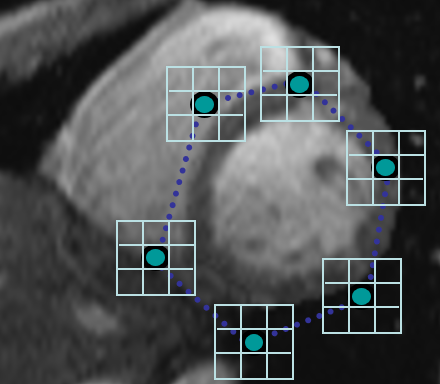
\includegraphics[height=3.2cm]{snakes/snake_w_windows_synth_1.PNG}
    \caption{Step $i$ of adjusting a snake with energy $E_i$.}
\end{figure}
\columnbreak
\begin{figure}[H]
	\centering %centralizar a figura
    	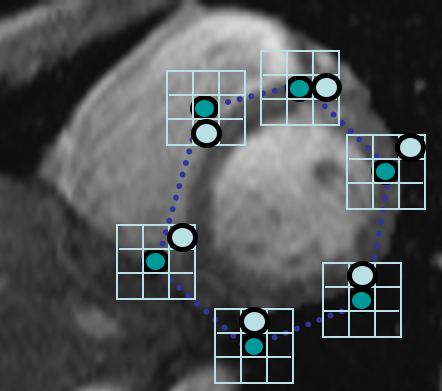
\includegraphics[height=3.2cm]{snakes/snake_w_windows_synth_2.PNG}
    \caption{Step $i$ of adjusting a snake with the points at an updated position in their window and energy $E_{i+1}<E_i$.}
\end{figure}
\end{multicols}
The main part of the greedy algorithm pseudocode as presented in Williams and Shah's paper \TODO[ref] is as follows. Note that the $ptsMoved$ variable simply counts the number of points moved, whose maximum allowed number is $thresh$. That is the stopping condition.
\begin{algorithm}[H] % H - use exact floating position
\caption{Snake energy minimisation simple greedy algorithm.}
\label{alg:ff_pseudo_final}
\begin{algorithmic}[1]
\Procedure{GreedySnake}{$img, points,thresh$} \Comment{thresh: \#times we're allowed to move points}
\State $\alpha\leftarrow 0.1,\ \beta\leftarrow 1.0,\ \gamma\leftarrow 0.1$ \Comment{example values}
\State $N \leftarrow$ number of points
\Do \Comment{loop to move points to new locations }
\For{$i=0,1,\ldots,n-1$}
\State $E_{min} \leftarrow \infty$
\For{$j=0,1,\ldots,m-1$} \Comment{Up to size of neighbourhood}
\State $E_j \leftarrow E_{int,i} + E_{ext,i}$ \Comment{Use values of $\alpha,\beta,\gamma$}
\If {$E_j < E_{min}$}
\State $E_{min} \leftarrow E_j$
\State $j_{min} \leftarrow j$
\EndIf
\EndFor
\State $point_i \leftarrow$ point at the location of $j_{min}$
\If{$j_{min}$ not in current location} \Comment{location of original point}
\State $ptsMoved++$
\EndIf
\EndFor
\doWhile{$ptsMoved < thresh$}
\EndProcedure
\end{algorithmic}
\end{algorithm}
% ref: http://scikit-image.org/docs/0.13.x/auto_examples/edges/plot_active_contours.html
Some ready to use source code for the greedy snake is found in App. \ref{app:snakes_code}. My own prototype of greedy snake minimisation written from scratch is also found in App. \ref{app:my_snakes_code}. A result of the prototype is shown below.\\


\begin{multicols}{2}
\begin{figure}[H]
	\centering %centralizar a figura
    	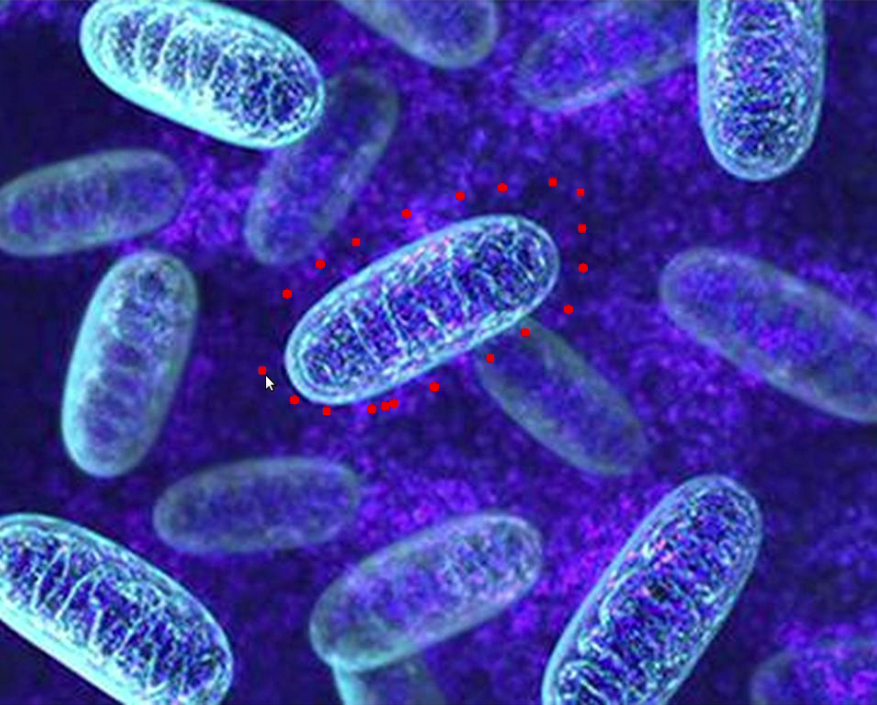
\includegraphics[height=3.6cm]{snakes/mysnakes_output_1.PNG}
    \caption{Initialisation of my snakes implementation; selecting the initial points loosely around a mitochondrion (red dots).}
\end{figure}
\columnbreak
\begin{figure}[H]
	\centering %centralizar a figura
    	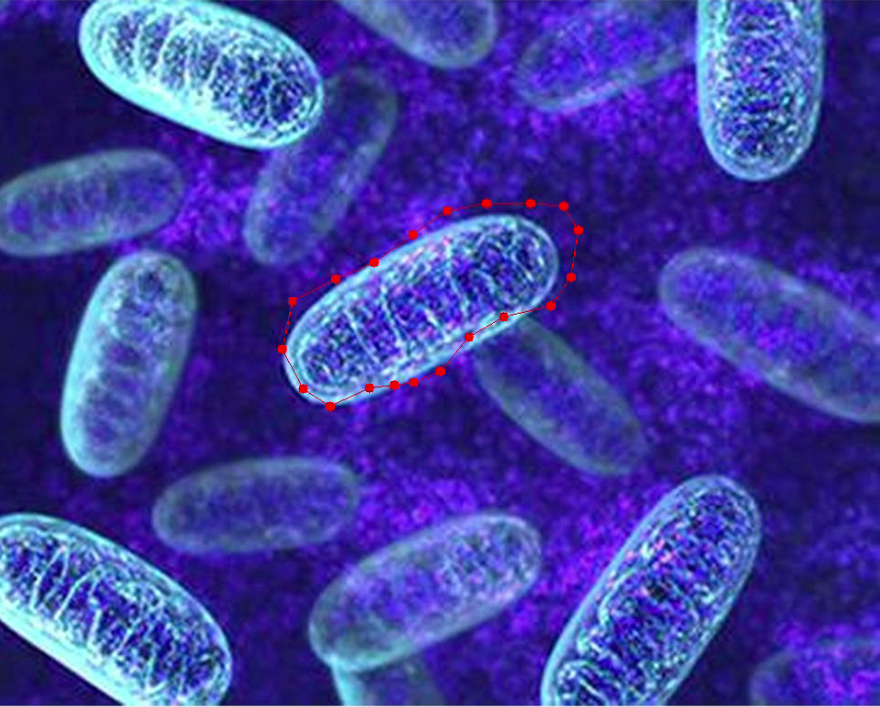
\includegraphics[height=3.6cm]{snakes/mysnakes_output_35.PNG}
    \caption{Final output after 35 iterations of my snake implementation for $\alpha=1.2, \ \beta = 1.0,\  \gamma = 0.45$. A tighter curve has been formed around the object.}
\end{figure}
\end{multicols}

\subsubsection{Advantages and disadvantages}
To summarise, for active contours we have found that:
% ref http://www.cs.cornell.edu/courses/cs664/2005fa/Lectures/lecture23.pdf
\begin{multicols}{2}
    \begin{itemize}
        \item[\textcolor{DarkPink}{\ding{51}}] Can be fine-tuned to fit the desired shaped using the energy function parameters.
        \item[\textcolor{DarkPink}{\ding{51}}] Can fit relatively complex shapes, in contrast e.g. with Hough transform - a popular shape detection technique.
    \end{itemize}
    
    \columnbreak
    \begin{itemize}
        \item[\textcolor{DarkPink}{\ding{55}}] High computation complexity - hard to use in real time.
        \item[\textcolor{DarkPink}{\ding{55}}] Can get stuck in local minimum.
        \item[\textcolor{DarkPink}{\ding{55}}] Often misses indentations in objects and hard to prevent self-intersections.
    \end{itemize}
\end{multicols}








% energy intution https://math.stackexchange.com/questions/904380/minimize-energy-in-image-processing-geodesic-active-contours













\section{Graph-based methods}

\subsection{Ford-Fulkerson algorithm}


\subsubsection{Introduction to graph cuts}

In this problem, the input is a directed graph $G(V,E)$, often called \emphasis{network} with a set of vertices $V$ and edges $E$. It contains two special vertices - the \emphasis{source} $s$ and \emphasis{target} $t$. We represent a directed edge $e$ from vertice $v$ to $u,\ v,u \in E$ as $(v,u)$. What's special about $s$ and $t$ is that there can only be edges flowing out of $s$, i.e. $(s,v), \ v \in V$ and only edges flowing in $t$, i.e. $(v,t),\ v \in V$, so $s$ generates material and $t$ absorbs it. Intuitively, the maximum flow problem takes a graph $G$ and sepeates it in two sets - one including $s$ and one $t$. It asks for the largest amount of material that can be transported from $s$ to $t$ across the cut; the minimum cut problem asks for the minimum damage needed to separate $s$ from $t$.\\
The following definition is therefore useful to study the problem given a graph $G=(V,E)$.
\begin{definition}
An \emphasis{s-t cut}, or simply \emphasis{cut} $(S,T)$ is a partition of vertices $V$ into two disjoint $S$ and $T=V \textbackslash S$ such that $s\in S$, $t \in T$, $S\cup T$=V, $S \cap T = \emptyset$.
\end{definition}



\subsubsection{Graph flows}

\begin{definition}An \emphasis{$(s,t)$-flow} (or just a \emphasis{flow} if the source and target are clear from context) is a function $f:E\mapsto \mathbb{R}\geq 0$ that satisfies the following \emphasis{conservation constraint} at every vertex v except possibly $s$ and $t$. It's the equivalent of Kirchhoff's 2nd law for graphs.
\begin{equation}
    \label{eq:conv_of_flow}
    \myunderbrace{\sum\limits_{u\in V}{f\left( u,v \right)}}{incoming}-
    \myunderbrace{\sum\limits_{u\in V}{f\left( v,u \right)}}{outgoing}=0,\ \ \forall v\in V \textbackslash \left\{ s,t \right\}
\end{equation}
\end{definition}
We also define the total flow, or simply flow, in a network as the amount of flow out of the source.
\begin{definition}
The value of the \emphasis{flow} in a network $G=(V,E)$ is 
\begin{equation}
    \left| f\right| = \sum\limits_{v\in V}{f\left( s,v \right)}
    \label{eq:def_total_flow}
\end{equation}
\end{definition}


\subsubsection{Flow value lemma}

Let $F = (G, s, t)$ be a flow graph (bidirectional, weighed), where $G=(V,E)$. The lemma below relates the total flow (\eqref{eq:def_total_flow}) in the graph to the net flow across any  $s-t$ cut $(S,T)$.
\begin{lemma}
\label{thm:flow_value}
Let $f$ be any flow, and let $(S,T)$ be any s-t cut. Then, the net flow sent across the cut is equal to the amount leaving $s$, i.e. 
\begin{equation}
    \label{eq:flow_value_lemma}
    \left|f \right| = f(S,T)
\end{equation}
\end{lemma}
\begin{proof}
Proof is found in App. \ref{app:flow_value_lemma_proof}.
\end{proof}

\begin{multicols}{2}
\begin{figure}[H]
	\centering %centralizar a figura
	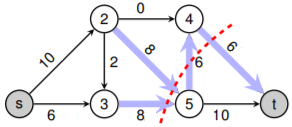
\includegraphics[width=0.35\textwidth]{flows/flow_val_numbers_1.png}
	\captionsetup{width=0.4\textwidth}
    \caption{Numerical demonstration of the lemma on a toy network. $S = \{s, "2", "3", "4"\},\ T=\{"5", t \}$, $\left|f \right| = 10+6$, $f(S,T) = 6 + 8 + 8 - 6 = \left| f \right|$}
\end{figure}

\columnbreak
\begin{figure}[H]
	\centering %centralizar a figura
	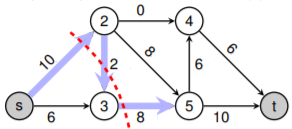
\includegraphics[width=.35\textwidth]{flows/flow_val_numbers_2.png}
	\captionsetup{width=0.4\textwidth}
        \caption{Numerical demonstration of the lemma on a toy network. $S = \{s, "3"\},\ T=\{"2", "4", "5", t \}$, $\left|f \right| = 10+6$, $f(S,T) = 10 + 8 - 2 = \left| f \right|$}
\end{figure}
\end{multicols}



\subsubsection{Flow graph capacity}

So far a network is considered as a graph $G=(V,E)$ with a source $s$ and a sink $t$, i.e. $F=(G,s,t)$. We add an additional parameter to the network model - the capacity $c$, therefore $F=(G,s,t,c)$. The capacity is the maximum flow an edge can carry, particularly;
\begin{definition}
\emphasis{Capacity} is a function that assigns a non-negative value to each edge that acts as an upper bound for its flow, i.e. $c:E\mapsto \mathbb{R}_{\geq 0}$. Therefore added to the conservation constraint in \eqref{eq:def_total_flow}, we have the capacity constraint for each edge $e=(u,v)$:
\begin{equation}
    \label{eq:capacity_constraint_edge}
    0 \leq f(e) \leq c(e)
\end{equation}
\end{definition}

\eqref{eq:conv_of_flow} and \eqref{eq:capacity_constraint_edge} are the fundamental equations that rule flow networks.

\begin{lemma}
If $(S,T)$ is an s-t cut across a network $F=G(G,s,t,c)$, then the capacity of the cut is the sum of capacities from set $S$ to set $T$.
\begin{equation}
    c(S,T) = \sum_{u\in S, \ v \in T}^{} c(u,v)
    \label{eq:def_cut_cap}
\end{equation}
\end{lemma}

% ref: https://inst.eecs.berkeley.edu/~cs170/fa16/lecture-10-13.pdf
\mycomment {The motivation for the definition is the following: let $S$ be the $S$ set of an $s-t$ cut in a network. Consider the set of edges
$(u,v) \in E:\ u\in S, \ v \notin T$. If we remove those edges from the network, then it is not possible to go from any vertex in $S$ to any vertex outside $S$ and, in particular, it is not possible to go from $s$ to $t$. This means that all the flow from $s$ to $t$ must pass through those edges, and so the total capacity of those edges (that, is $c(S)$) is an upper bound to the cost of any feasible flow. \\
% redf http://www.cs.tufts.edu/~cowen/advanced/lect3-final.pdf
Therefore, while the capacities of different cuts may be different, the total value of flow across a cut boundary is always constant. This provides intuition to the following conclusion that can be proven rigorously.}
\begin{lemma}
\label{thm:weak_duality}
Let $f$ be the flow value and $(S,T)$ be any cut. Then the value of $f$ is bounded from above by the capacity of the cut $(S,T)$, i.e.,
\begin{equation}
    \left|f \right| \leq c(S,T)
\end{equation}
\end{lemma}
\begin{proof}
\begin{align}
    \left|f \right| &= 	\sum\limits_{(u,v)\in E(S,T)}{f\left( u,v \right)}-\sum\limits_{(v,u)\in E(T,S)}{f\left( v,u \right)} \tag{1} \\
                    &\leq  \sum\limits_{(u,v)\in E(S,T)}{f\left( u,v \right)} \tag{2} \\
                    &\leq  \sum\limits_{(u,v)\in E(S,T)}{c\left( u,v \right)} \tag{3}
\end{align}
Eq. (1) follows from the the flow value lemma (\eqref{eq:flow_value_lemma}) and (3) from the capacity constraint.
\end{proof}



\subsubsection{Residual network and Augmenting Path}

% ref https://www.geeksforgeeks.org/ford-fulkerson-algorithm-for-maximum-flow-problem/
% ref https://www.coursera.org/lecture/advanced-algorithms-and-complexity/residual-networks-TIGj4
Residual network is an auxiliary graph that depends on the original graph $G$ and its current flow $f$ where the FFA operates on. As motivated in \ref{app:ffa_motivation}, it captures the extra flow that can be passed along each edge and the direction where it can be passed.
% ref https://web.cs.hacettepe.edu.tr/~ozkahya/classes/bbm402/Lectures/Lec16-flowalgo.pdf
% ref http://ac.informatik.uni-freiburg.de/teaching/ws12_13/algotheo/Slides/pdf/05_GraphAlgorithms_komplett.pdf
\begin{definition}
Given a network $G=(V,E,c)$ and flow $f$, the \emphasis{residual graph} $G_f=(V_f, E_f, c_f)$  of $G$ with respect to $f$ $G_f = (V_f,E_f)$:
\begin{itemize}
    \item has node set $V_f=V$
    \item For each edge $(u,v) \in E$ there are two edges in $E_f$:
    \begin{itemize}
        \item forward edge $e=(u,v)$ with \emphasis{residual capacity} $c_e - f(e)$
        \item backward edge $e'=(v,u)$ with \emphasis{residual capacity} $f(e)$
    \end{itemize}
\end{itemize}
\end{definition}

\mycomment{If for an  edge $e\in E$ $f(e)=c_f$, then the forward edge on the residual graph has $0$ capacity, so we don't need to consider and only one (backward) edge needs to be draw in the residual graph.}
Therefore the residual capacity is formally defined as
\begin{equation}
  c_f(u,v) =
  \begin{cases}
     c(u,v) - f(u,v)  & \text{if $ (u,v) \in E$} \\
     f(v,u) & \text{if $ (v,u) \in E$} \\
     0 & \text{otherwise}
  \end{cases}\
  \label{eq:resid_capacity}
\end{equation}
% ref http://www.cs.umd.edu/class/fall2017/cmsc451-0101/Lects/lect15-flow-ford-fulk.pdf


An example of finding the residual network according to \eqref{eq:resid_capacity} is shown below.

\begin{figure}[H]
	\centering %centralizar a figura
	\label{fig:resid_network_example}
	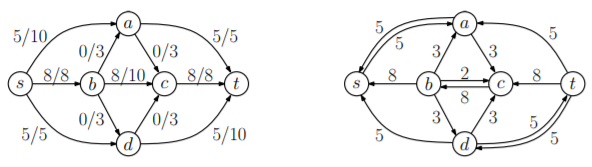
\includegraphics[height=3.4cm]{flows/resid_network_example.PNG}
        \caption{An example network (left) and its residual network (right)}
\end{figure}



\begin{definition}
An \emphasis{augmenting path} $P$ is a simple (non cyclic) $s-t$ path on the residual network $G_f$ on which each edge has residual capacity $c_f>0$.
\end{definition}
\begin{definition}
\emphasis{bottleneck}$(P,f)$ is the minimum residual capacity on any edge of the augmenting path.
\end{definition}
\begin{corollary}
When augmenting the flow along a path $P$
\begin{itemize}
    \item For every forward edge $(u,v)$ along $P$:
    \begin{equation*}
        f'\left((u,v)\right) = f\left((u,v)\right) + \textup{bottleneck}(P,f)
    \end{equation*}
    \item For every backward edge $(u,v)$ along $P$:
    \begin{equation*}
        f'\left((u,v)\right) = f\left((u,v)\right) - \textup{bottleneck}(P,f)
    \end{equation*}
\end{itemize}
\end{corollary}
\mycomment{The signs are chosen this way so that they comply with the conservation of flow.}



\subsubsection{Ford–Fulkerson algorithm}
The Ford–Fulkerson algorithm (FFA) is a greedy algorithm that computes the maximum flow and the maximum flow cut in a flow network. An initial idea for a greedy maximum flow algorithm that motivates FFA is presented in \ref{app:ffa_motivation}.\\
%%%%%%%%%%%%%%%
% moved to app.
%%%%%%%%%%%%%%
FFA utilises the residual graph $G_f$ and updates it at each iteration. The final pseudocode is listed below.


% before the algo - see here https://web.cs.hacettepe.edu.tr/~ozkahya/classes/bbm402/Lectures/Lec16-flowalgo.pdf
%%%%%%%%%%%%%%%% algo src %%%%%%%%%%%%%%%
% http://www.cse.unt.edu/~tarau/teaching/AnAlgo/Ford%E2%80%93Fulkerson%20algorithm.pdf
% https://stackoverflow.com/questions/7741077/ford-fulkerson-from-cormen-et-al
% http://courses.cs.vt.edu/cs5114/spring2009/lectures/lecture18-network-flow.pdf  pseudo+res

The approach is loosely outlined below.
% ref https://people.eecs.berkeley.edu/~daw/teaching/cs170-s03/Notes/lecture19.pdf
\begin{verbatim}
Given in input G = (V, E), vertices s, t, and capacities c(u,v).
1.Initialize f(u,v) to zero for all edges.
2. Use Depth-First Search to find a path from s to t. If no path is found, return the current flow.
3. Let b be the smallest ("bottleneck") capacity along the path.
4. For each edge (u, v) in the path
    decrease c(u,v) by b
    increase f(u,v) by b, and increase
    c(v,u) by b (if the edge (v, u) does not exist in G, create it).
    Delete edges with capacity zero.
5. Go to step (2)
\end{verbatim}

A more concrete pseudocode is listed below.
% ref https://web.cs.hacettepe.edu.tr/~ozkahya/classes/bbm402/Lectures/Lec16-flowalgo.pdf
% ref http://ac.informatik.uni-freiburg.de/teaching/ws12_13/algotheo/Slides/pdf/05_GraphAlgorithms_komplett.pdf
%%%%%%%%%%%%%%%%%%%%%%%%%%%%%%%%%%%%%%%%
\begin{algorithm}[H] % H - use exact floating position
\caption{Ford Fuklkerson complete pseudocode}
\label{alg:ff_pseudo_final}
\begin{algorithmic}[1]
\Procedure{bottleneck}{$P,f$}
\State \textbf{Return} $\underset{e\in E\left( P \right)}{\mathop{\min }}\,c\left( e \right)$ 
\EndProcedure
\State

\Procedure{augment}{$f, P$}
\Comment{$f$: flow, $P$:path}
\For {each edge $(u,v) \in P$}
\If {$e=(u,v)$ is a forward edge} \Comment{forward w.r.t. $P$}
\State $f(e) = f(e) + b$
\EndIf
\If {$(u,v)$ is a backward edge} 
\State \textbf{let} $e \leftarrow (v,u)$ \Comment{as long as $(v,u) \in G$}
\State $f(e) = f(e) - b$
\EndIf
\EndFor
\State \textbf{return} $f$
\EndProcedure

\State
\Procedure{FordFulkerson}{$G,s,t,c$}
\For {each edge $e\in G$}
\State \textbf{let} $c_{Gf}(u,v) \leftarrow f((u,v))$ \Comment{Initialise residual graph}
\State $f_{Gf}(e)=0$
\EndFor
\While{$G_f$ has a simple $s-t$ path}
\State \textbf{let} $P\leftarrow$ a simple $s-t$ path in $G_f$ \Comment{Find it e.g. by DFS}
\State \textbf{let} $f\leftarrow \textsc{augment}(f,P)$
\State \textbf{update} the residual graph $G_f$
\EndWhile
\State \textbf{return} $f$
\EndProcedure
\end{algorithmic}
\end{algorithm}

A step by step run of FFA is shown in Table \ref{tab:ffa_step_by_step}.


% example http://service.hidebux.com/index.php?q=n9XX1dhrZ5GgoJ6p1WSW0NJixGatx9WHqg
% other exmp http://www14.in.tum.de/lehre/2015WS/ea/split/sub-The-Generic-Augmenting-Path-Algorithm.pdf

\begin{minipage}{\linewidth}
\captionof{table}{FFA step-by-step example with the augmented and residual graph per step shown.} 
\begin{center}
\label{tab:ffa_step_by_step}
\begin{tabular}{| m{.35\textwidth} | m{.35\textwidth} | m{.2\textwidth} |}
\hline   
% image, rank, output, n required, norm 2 of difference, Singular value of rank r+1
    \textbf{Augmented} & \textbf{Residual} & \textbf{Comments}\\
\hline 
\hline 
    \usetikzlibrary{arrows, quotes}
%\newcommand{\bluebold}[1]{\textbf{\textcolor{blue}{#1}}} % text above = symbol

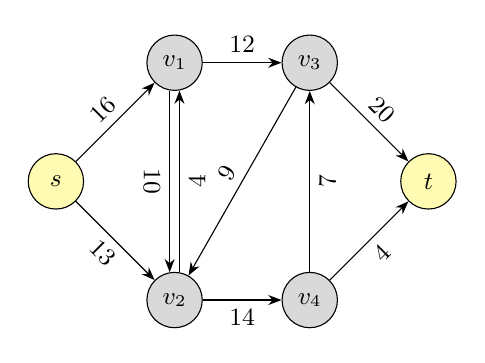
\begin{tikzpicture}[
      circle_st/.style={
         circle,
         draw=black,
         fill=yellow,
         fill opacity = 0.3,
         text opacity=1,
         inner sep=0pt,
         minimum size=20pt,
         font=\small},
       circle_node/.style={
         circle,
         draw=black,
         fill=gray,
         fill opacity = 0.3,
         text opacity=1,
         inner sep=0pt,
         minimum size=20pt,
         font=\small} ,
       arrow_black/.style={
        -Stealth,
        },
        arrow_bold/.style={
        -Stealth,
        fill=red,
        line width=0.25mm,
        draw = red,
        }
]	
      %source
      \node[circle_st] (s) {$s$};
      
      \node[circle_node,above right=of s] (v1) {$v_1$};
      \node[circle_node,below right=of s] (v2) {$v_2$};
      
      \node[circle_node,right=of v1] (v3) {$v_3$};
      \node[circle_node,right=of v2] (v4) {$v_4$};
      
      \node[circle_st,below right=of v3] (t) {$t$};


    \foreach \i/\j/\txt/\p in {% start node/end node/text/position
      s/v1/16/above,
      s/v2/13/below,
      v1.260/v2.100/$10$/below,
      v2.80/v1.280/$4$/below,
      v1/v3/$12$/above,
      v2/v4/$14$/below,
      v3/v2/$9$/above,
      v4/v3/$7$/below,
      v3/t/$20$/above,
      v4/t/$4$/below}
      \draw [arrow_black] (\i) -- node[sloped,font=\small,\p] {\txt} (\j);

\end{tikzpicture} &
    \usetikzlibrary{arrows, quotes}
%\newcommand{\bluebold}[1]{\textbf{\textcolor{blue}{#1}}} % text above = symbol

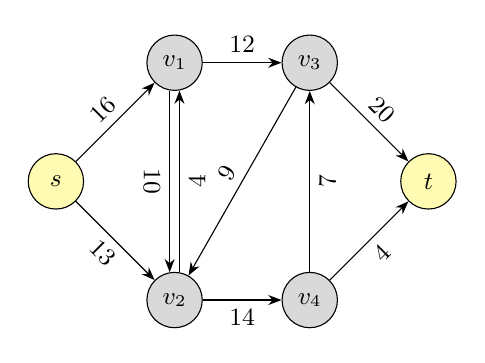
\begin{tikzpicture}[
      circle_st/.style={
         circle,
         draw=black,
         fill=yellow,
         fill opacity = 0.3,
         text opacity=1,
         inner sep=0pt,
         minimum size=20pt,
         font=\small},
       circle_node/.style={
         circle,
         draw=black,
         fill=gray,
         fill opacity = 0.3,
         text opacity=1,
         inner sep=0pt,
         minimum size=20pt,
         font=\small} ,
       arrow_black/.style={
        -Stealth,
        },
        arrow_bold/.style={
        -Stealth,
        fill=red,
        line width=0.25mm,
        draw = red,
        }
]	
      %source
      \node[circle_st] (s) {$s$};
      
      \node[circle_node,above right=of s] (v1) {$v_1$};
      \node[circle_node,below right=of s] (v2) {$v_2$};
      
      \node[circle_node,right=of v1] (v3) {$v_3$};
      \node[circle_node,right=of v2] (v4) {$v_4$};
      
      \node[circle_st,below right=of v3] (t) {$t$};
    
    \foreach \i/\j/\txt/\p in {% start node/end node/text/position
      s/v1/16/above,
      s/v2/13/below,
      v1.260/v2.100/$10$/below,
      v2.80/v1.280/$4$/below,
      v1/v3/$12$/above,
      v2/v4/$14$/below,
      v3/v2/$9$/above,
      v4/v3/$7$/below,
      v3/t/$20$/above,
      v4/t/$4$/below}
      \draw [arrow_black] (\i) -- node[sloped,font=\small,\p] {\txt} (\j);



\end{tikzpicture} &
    Initialisation step; The augmented graph has some capacities and zero flows and the residual the same capacities as the augmented\\
\hline 
    \usetikzlibrary{arrows, quotes}
%\newcommand{\bluebold}[1]{\textbf{\textcolor{blue}{#1}}} % text above = symbol

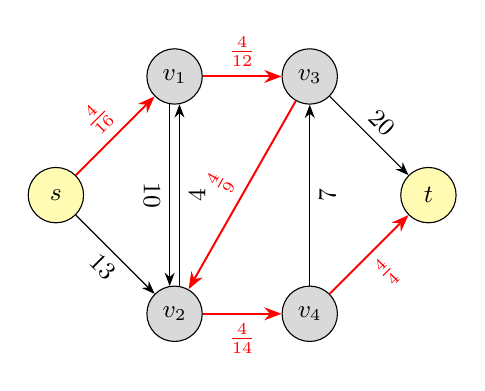
\begin{tikzpicture}[
      circle_st/.style={
         circle,
         draw=black,
         fill=yellow,
         fill opacity = 0.3,
         text opacity=1,
         inner sep=0pt,
         minimum size=20pt,
         font=\small},
       circle_node/.style={
         circle,
         draw=black,
         fill=gray,
         fill opacity = 0.3,
         text opacity=1,
         inner sep=0pt,
         minimum size=20pt,
         font=\small} ,
       arrow_black/.style={
        -Stealth,
        },
       arrow_bold/.style={
        -Stealth,
        fill=red,
        line width=0.25mm,
        draw = red,
        }
]	
      %source
      \node[circle_st] (s) {$s$};
      
      \node[circle_node,above right=of s] (v1) {$v_1$};
      \node[circle_node,below right=of s] (v2) {$v_2$};
      
      \node[circle_node,right=of v1] (v3) {$v_3$};
      \node[circle_node,right=of v2] (v4) {$v_4$};
      
      \node[circle_st,below right=of v3] (t) {$t$};
    
    \foreach \i/\j/\txt/\p in {% start node/end node/text/position
      %s/v1/16/above,
      s/v2/13/below,
      v1.260/v2.100/$10$/below,
      v2.80/v1.280/$4$/below,
      %v1/v3/$12$/above,
      %v2/v4/$14$/below,
      %v3/v2/$9$/above,
      v4/v3/$7$/below,
      v3/t/$20$/above}
      \draw [arrow_black] (\i) -- node[sloped,font=\small,\p] {\txt} (\j);
    
    \foreach \i/\j/\txt/\p in {% start node/end node/text/position
      s/v1/$\textcolor{red}{\tfrac{4}{16}}$/above,
      %s/v2/13/below,
      %v1.260/v2.100/$10$/below,
      %v2.80/v1.280/$4$/below,
      v1/v3/$\textcolor{red}{\tfrac{4}{12}}$/above,
      v2/v4/$\textcolor{red}{\tfrac{4}{14}}$/below,
      v3/v2/$\textcolor{red}{\tfrac{4}{9}}$/above,
      v4/t/$\textcolor{red}{\tfrac{4}{4}}$/below}
      \draw [arrow_bold] (\i) -- node[sloped,font=\small,\p] {\txt} (\j);  
    



\end{tikzpicture} &
    \usetikzlibrary{arrows, quotes}
%\newcommand{\bluebold}[1]{\textbf{\textcolor{blue}{#1}}} % text above = symbol

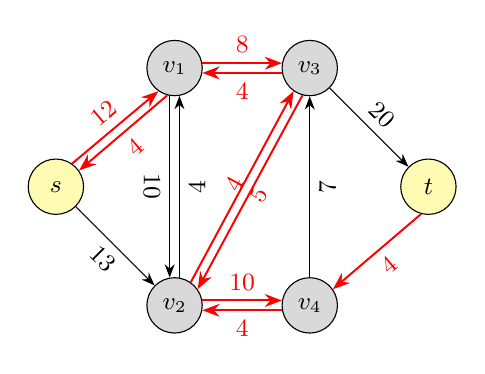
\begin{tikzpicture}[
      circle_st/.style={
         circle,
         draw=black,
         fill=yellow,
         fill opacity = 0.3,
         text opacity=1,
         inner sep=0pt,
         minimum size=20pt,
         font=\small},
       circle_node/.style={
         circle,
         draw=black,
         fill=gray,
         fill opacity = 0.3,
         text opacity=1,
         inner sep=0pt,
         minimum size=20pt,
         font=\small} ,
       arrow_black/.style={
        -Stealth,
        },
       arrow_bold/.style={
        -Stealth,
        fill=red,
        line width=0.25mm,
        draw = red,
        }
]	
      %source
      \node[circle_st] (s) {$s$};
      
      \node[circle_node,above right=of s] (v1) {$v_1$};
      \node[circle_node,below right=of s] (v2) {$v_2$};
      
      \node[circle_node,right=of v1] (v3) {$v_3$};
      \node[circle_node,right=of v2] (v4) {$v_4$};
      
      \node[circle_st,below right=of v3] (t) {$t$};
    
    \foreach \i/\j/\txt/\p in {% start node/end node/text/position
      %s/v1/16/above,
      s/v2/13/below,
      v1.260/v2.100/$10$/below,
      v2.80/v1.280/$4$/below,
      %v1/v3/$12$/above,
      %v2/v4/$14$/below,
      %v3/v2/$9$/above,
      v4/v3/$7$/below,
      v3/t/$20$/above}
      \draw [arrow_black] (\i) -- node[sloped,font=\small,\p] {\txt} (\j);
    
    \foreach \i/\j/\txt/\p in {% start node/end node/text/position
      s.55/v1.235/$\textcolor{red}{12}$/above,
      v1.255/s.35/$\textcolor{red}{4}$/below,
      %s/v2/13/below,
      %v1.260/v2.100/$10$/below,
      %v2.80/v1.280/$4$/below,
      v1.10/v3.170/$\textcolor{red}{8}$/above,
      v3.190/v1.350/$\textcolor{red}{4}$/below,
      v3.255/v2.35/$\textcolor{red}{4}$/above,
      v2.55/v3.235/$\textcolor{red}{5}$/below,
      v2.10/v4.170/$\textcolor{red}{10}$/above,
      v4.190/v2.350/$\textcolor{red}{4}$/below,
      t.255/v4.35/$\textcolor{red}{4}$/below}
      \draw [arrow_bold] (\i) -- node[sloped,font=\small,\p] {\txt} (\j);  
    



\end{tikzpicture} &
    $f=4$ (along $(4,t)$)\\
\hline 
    \usetikzlibrary{arrows, quotes}
%\newcommand{\bluebold}[1]{\textbf{\textcolor{blue}{#1}}} % text above = symbol

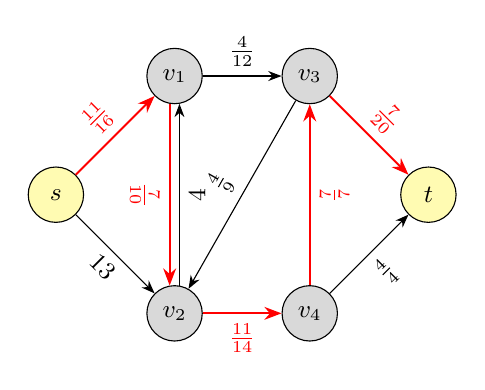
\begin{tikzpicture}[
      circle_st/.style={
         circle,
         draw=black,
         fill=yellow,
         fill opacity = 0.3,
         text opacity=1,
         inner sep=0pt,
         minimum size=20pt,
         font=\small},
       circle_node/.style={
         circle,
         draw=black,
         fill=gray,
         fill opacity = 0.3,
         text opacity=1,
         inner sep=0pt,
         minimum size=20pt,
         font=\small} ,
       arrow_black/.style={
        -Stealth,
        },
        arrow_bold/.style={
        -Stealth,
        fill=red,
        line width=0.25mm,
        draw = red,
        }
]	
      %source
      \node[circle_st] (s) {$s$};
      
      \node[circle_node,above right=of s] (v1) {$v_1$};
      \node[circle_node,below right=of s] (v2) {$v_2$};
      
      \node[circle_node,right=of v1] (v3) {$v_3$};
      \node[circle_node,right=of v2] (v4) {$v_4$};
      
      \node[circle_st,below right=of v3] (t) {$t$};
      
    \foreach \i/\j/\txt/\p in {% start node/end node/text/position
      %s/v1/16/above,
      s/v2/13/below,
      v2.80/v1.280/$4$/below,
      %v1/v3/$12$/above,
      %v2/v4/$14$/below,
      %v3/v2/$9$/above,
      %s/v2/13/below,
      %v1.260/v2.100/$10$/below,
      %v2.80/v1.280/$4$/below,
      v1/v3/$\textcolor{black}{\tfrac{4}{12}}$/above,
      v3/v2/$\textcolor{black}{\tfrac{4}{9}}$/above,
      v4/t/$\textcolor{black}{\tfrac{4}{4}}$/below}
      \draw [arrow_black] (\i) -- node[sloped,font=\small,\p] {\txt} (\j);  
     
     \foreach \i/\j/\txt/\p in {% start
       v1.260/v2.100/$\textcolor{red}{\tfrac{7}{10}}$/below,
             v3/t/$\textcolor{red}{\tfrac{7}{20}}$/above,
       v2/v4/$\textcolor{red}{\tfrac{11}{14}}$/below,    
       v4/v3/$\textcolor{red}{\tfrac{7}{7}}$/below,
       s/v1/$\textcolor{red}{\tfrac{11}{16}}$/above}
 \draw [arrow_bold] (\i) -- node[sloped,font=\small,\p] {\txt} (\j);  


\end{tikzpicture} &
    \usetikzlibrary{arrows, quotes}
%\newcommand{\bluebold}[1]{\textbf{\textcolor{blue}{#1}}} % text above = symbol

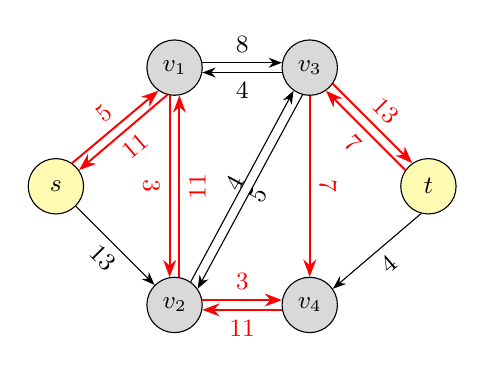
\begin{tikzpicture}[
      circle_st/.style={
         circle,
         draw=black,
         fill=yellow,
         fill opacity = 0.3,
         text opacity=1,
         inner sep=0pt,
         minimum size=20pt,
         font=\small},
       circle_node/.style={
         circle,
         draw=black,
         fill=gray,
         fill opacity = 0.3,
         text opacity=1,
         inner sep=0pt,
         minimum size=20pt,
         font=\small} ,
       arrow_black/.style={
        -Stealth,
        },
       arrow_bold/.style={
        -Stealth,
        fill=red,
        line width=0.25mm,
        draw = red,
        }
]	
      %source
      \node[circle_st] (s) {$s$};
      
      \node[circle_node,above right=of s] (v1) {$v_1$};
      \node[circle_node,below right=of s] (v2) {$v_2$};
      
      \node[circle_node,right=of v1] (v3) {$v_3$};
      \node[circle_node,right=of v2] (v4) {$v_4$};
      
      \node[circle_st,below right=of v3] (t) {$t$};
    
    \foreach \i/\j/\txt/\p in {% start node/end node/text/position
      %s/v1/16/above,
      s/v2/13/below,
      %v1/v3/$12$/above,
      %v2/v4/$14$/below,
      %v3/v2/$9$/above,
      %s/v2/13/below,
      %v1.260/v2.100/$3$/below,
      %v2.80/v1.280/$11$/below,
      v1.10/v3.170/$\textcolor{black}{8}$/above,
      v3.190/v1.350/$\textcolor{black}{4}$/below,
      v3.255/v2.35/$\textcolor{black}{4}$/above,
      v2.55/v3.235/$\textcolor{black}{5}$/below,
      t.255/v4.35/$\textcolor{black}{4}$/below}
      \draw [arrow_black] (\i) -- node[sloped,font=\small,\p] {\txt} (\j);  
    
    \foreach \i/\j/\txt/\p in {% start node/end node/text/position
      s.55/v1.235/$\textcolor{red}{5}$/above,
      v1.255/s.35/$\textcolor{red}{11}$/below,
      v3/v4/$\textcolor{red}{7}$/above,
      v2.10/v4.170/$\textcolor{red}{3}$/above,
      v4.190/v2.350/$\textcolor{red}{11}$/below,
      v3.325/t.125/$\textcolor{red}{13}$/above,
      v1.260/v2.100/$\textcolor{red}{3}$/below,
      v2.80/v1.280/$\textcolor{red}{11}$/below,
      t.145/v3.305/$\textcolor{red}{7}$/below}
    \draw [arrow_bold] (\i) -- node[sloped,font=\small,\p] {\txt} (\j);  


\end{tikzpicture} &
    $f=7$ along $(4,3)$\\
\hline 
    \usetikzlibrary{arrows, quotes}
%\newcommand{\bluebold}[1]{\textbf{\textcolor{blue}{#1}}} % text above = symbol

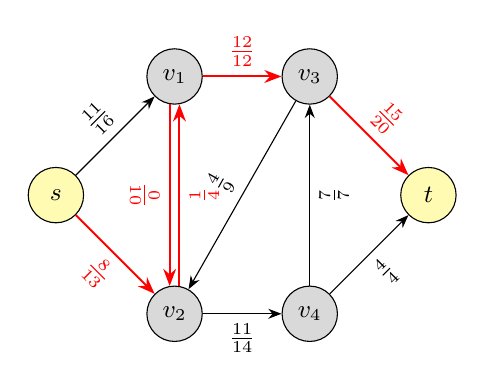
\begin{tikzpicture}[
      circle_st/.style={
         circle,
         draw=black,
         fill=yellow,
         fill opacity = 0.3,
         text opacity=1,
         inner sep=0pt,
         minimum size=20pt,
         font=\small},
       circle_node/.style={
         circle,
         draw=black,
         fill=gray,
         fill opacity = 0.3,
         text opacity=1,
         inner sep=0pt,
         minimum size=20pt,
         font=\small} ,
       arrow_black/.style={
        -Stealth,
        },
        arrow_bold/.style={
        -Stealth,
        fill=red,
        line width=0.25mm,
        draw = red,
        }
]	
      %source
      \node[circle_st] (s) {$s$};
      
      \node[circle_node,above right=of s] (v1) {$v_1$};
      \node[circle_node,below right=of s] (v2) {$v_2$};
      
      \node[circle_node,right=of v1] (v3) {$v_3$};
      \node[circle_node,right=of v2] (v4) {$v_4$};
      
      \node[circle_st,below right=of v3] (t) {$t$};
      
    \foreach \i/\j/\txt/\p in {% start node/end node/text/position
      %s/v1/16/above,
      v3/v2/$\textcolor{black}{\tfrac{4}{9}}$/above,
      v4/t/$\textcolor{black}{\tfrac{4}{4}}$/below,
       v2/v4/$\textcolor{black}{\tfrac{11}{14}}$/below,    
       v4/v3/$\textcolor{black}{\tfrac{7}{7}}$/below,
       s/v1/$\textcolor{black}{\tfrac{11}{16}}$/above}
 \draw [arrow_black] (\i) -- node[sloped,font=\small,\p] {\txt} (\j);  
 
 \foreach \i/\j/\txt/\p in {% start node/end node/text/position
    s/v2/$\textcolor{red}{\tfrac{8}{13}}$/below,
    v1/v3/$\textcolor{red}{\tfrac{12}{12}}$/above,
    v1.260/v2.100/$\textcolor{red}{\tfrac{0}{10}}$/below,
    v2.80/v1.280/$\textcolor{red}{\tfrac{1}{4}}$/below,
    v3/t/$\textcolor{red}{\tfrac{15}{20}}$/above}
\draw [arrow_bold] (\i) -- node[sloped,font=\small,\p] {\txt} (\j);  
\end{tikzpicture} &
    \usetikzlibrary{arrows, quotes}
%\newcommand{\bluebold}[1]{\textbf{\textcolor{blue}{#1}}} % text above = symbol

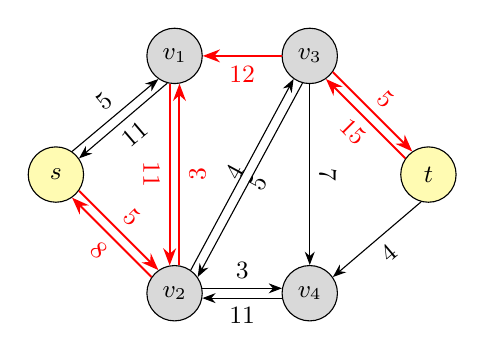
\begin{tikzpicture}[
      circle_st/.style={
         circle,
         draw=black,
         fill=yellow,
         fill opacity = 0.3,
         text opacity=1,
         inner sep=0pt,
         minimum size=20pt,
         font=\small},
       circle_node/.style={
         circle,
         draw=black,
         fill=gray,
         fill opacity = 0.3,
         text opacity=1,
         inner sep=0pt,
         minimum size=20pt,
         font=\small} ,
       arrow_black/.style={
        -Stealth,
        },
        arrow_bold/.style={
        -Stealth,
        fill=red,
        line width=0.25mm,
        draw = red,
        }
]	
      %source
      \node[circle_st] (s) {$s$};
      
      \node[circle_node,above right=of s] (v1) {$v_1$};
      \node[circle_node,below right=of s] (v2) {$v_2$};
      
      \node[circle_node,right=of v1] (v3) {$v_3$};
      \node[circle_node,right=of v2] (v4) {$v_4$};
      
      \node[circle_st,below right=of v3] (t) {$t$};

    \foreach \i/\j/\txt/\p in {% start node/end node/text/position
      v3.255/v2.35/$\textcolor{black}{4}$/above,
      v2.55/v3.235/$\textcolor{black}{5}$/below,
      t.255/v4.35/$\textcolor{black}{4}$/below,
      s.55/v1.235/$\textcolor{black}{5}$/above,
      v1.255/s.35/$\textcolor{black}{11}$/below,
      v3/v4/$\textcolor{black}{7}$/above,
      v2.10/v4.170/$\textcolor{black}{3}$/above,
      v4.190/v2.350/$\textcolor{black}{11}$/below}
    \draw [arrow_black] (\i) -- node[sloped,font=\small,\p] {\txt} (\j);  
    
    \foreach \i/\j/\txt/\p in {% start node/end
      v3/v1/$\textcolor{red}{12}$/below,
      s.325/v2.125/$\textcolor{red}{5}$/above,
      v2.145/s.305/$\textcolor{red}{8}$/below,
      v3.325/t.125/$\textcolor{red}{5}$/above,
      v1.260/v2.100/$\textcolor{red}{11}$/below,
      v2.80/v1.280/$\textcolor{red}{3}$/below,
      t.145/v3.305/$\textcolor{red}{15}$/below}
    \draw [arrow_bold] (\i) -- node[sloped,font=\small,\p] {\txt} (\j); 

\end{tikzpicture} &
    $f=8$; look at augmented above, (1,3) can support up to 8 and of course (2,1) can take 8 - 7 against (1,2) and anoteher 1/4 from (2,1)\\
\hline 
    \usetikzlibrary{arrows, quotes}
%\newcommand{\bluebold}[1]{\textbf{\textcolor{blue}{#1}}} % text above = symbol

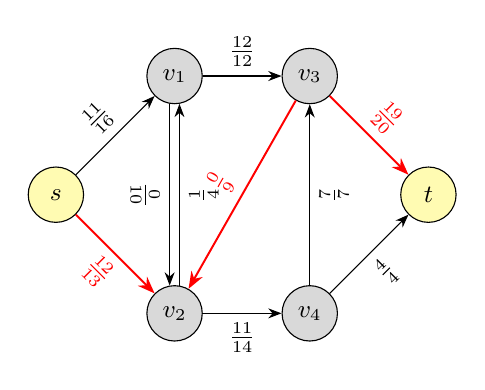
\begin{tikzpicture}[
      circle_st/.style={
         circle,
         draw=black,
         fill=yellow,
         fill opacity = 0.3,
         text opacity=1,
         inner sep=0pt,
         minimum size=20pt,
         font=\small},
       circle_node/.style={
         circle,
         draw=black,
         fill=gray,
         fill opacity = 0.3,
         text opacity=1,
         inner sep=0pt,
         minimum size=20pt,
         font=\small} ,
       arrow_black/.style={
        -Stealth,
        },
        arrow_bold/.style={
        -Stealth,
        fill=red,
        line width=0.25mm,
        draw = red,
        }
]	
      %source
      \node[circle_st] (s) {$s$};
      
      \node[circle_node,above right=of s] (v1) {$v_1$};
      \node[circle_node,below right=of s] (v2) {$v_2$};
      
      \node[circle_node,right=of v1] (v3) {$v_3$};
      \node[circle_node,right=of v2] (v4) {$v_4$};
      
      \node[circle_st,below right=of v3] (t) {$t$};
      
    \foreach \i/\j/\txt/\p in {% start node/end node/text/position
      %s/v1/16/above,
      v4/t/$\textcolor{black}{\tfrac{4}{4}}$/below,
       v2/v4/$\textcolor{black}{\tfrac{11}{14}}$/below,    
       v4/v3/$\textcolor{black}{\tfrac{7}{7}}$/below,
       s/v1/$\textcolor{black}{\tfrac{11}{16}}$/above,
      v1/v3/$\textcolor{black}{\tfrac{12}{12}}$/above,
      v1.260/v2.100/$\textcolor{black}{\tfrac{0}{10}}$/below,
      v2.80/v1.280/$\textcolor{black}{\tfrac{1}{4}}$/below}
      \draw [arrow_black] (\i) -- node[sloped,font=\small,\p] {\txt} (\j);  
      
     \foreach \i/\j/\txt/\p in { 
       s/v2/$\textcolor{red}{\tfrac{12}{13}}$/below,
       v3/v2/$\textcolor{red}{\tfrac{0}{9}}$/above,
       v3/t/$\textcolor{red}{\tfrac{19}{20}}$/above}
       \draw [arrow_bold] (\i) -- node[sloped,font=\small,\p] {\txt} (\j); 
\end{tikzpicture} &
    \usetikzlibrary{arrows, quotes}
%\newcommand{\bluebold}[1]{\textbf{\textcolor{blue}{#1}}} % text above = symbol

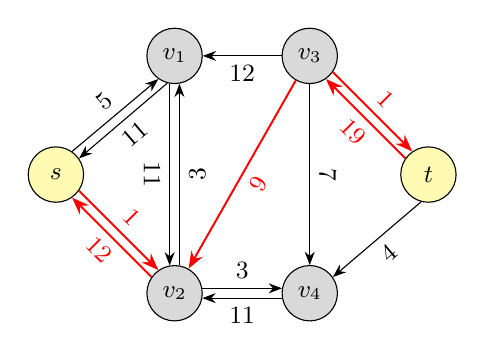
\begin{tikzpicture}[
      circle_st/.style={
         circle,
         draw=black,
         fill=yellow,
         fill opacity = 0.3,
         text opacity=1,
         inner sep=0pt,
         minimum size=20pt,
         font=\small},
       circle_node/.style={
         circle,
         draw=black,
         fill=gray,
         fill opacity = 0.3,
         text opacity=1,
         inner sep=0pt,
         minimum size=20pt,
         font=\small} ,
       arrow_black/.style={
        -Stealth,
        },
        arrow_bold/.style={
        -Stealth,
        fill=red,
        line width=0.25mm,
        draw = red,
        }
]	
      %source
      \node[circle_st] (s) {$s$};
      
      \node[circle_node,above right=of s] (v1) {$v_1$};
      \node[circle_node,below right=of s] (v2) {$v_2$};
      
      \node[circle_node,right=of v1] (v3) {$v_3$};
      \node[circle_node,right=of v2] (v4) {$v_4$};
      
      \node[circle_st,below right=of v3] (t) {$t$};

    \foreach \i/\j/\txt/\p in {% start node/end node/text/position
      t.255/v4.35/$\textcolor{black}{4}$/below,
      s.55/v1.235/$\textcolor{black}{5}$/above,
      v1.255/s.35/$\textcolor{black}{11}$/below,
      v3/v4/$\textcolor{black}{7}$/above,
      v2.10/v4.170/$\textcolor{black}{3}$/above,
      v4.190/v2.350/$\textcolor{black}{11}$/below,
      v3/v1/$\textcolor{black}{12}$/below,
      v1.260/v2.100/$\textcolor{black}{11}$/below,
      v2.80/v1.280/$\textcolor{black}{3}$/below}
    \draw [arrow_black] (\i) -- node[sloped,font=\small,\p] {\txt} (\j); 
    
    \foreach \i/\j/\txt/\p in {% start node/end node/text/position
      s.325/v2.125/$\textcolor{red}{1}$/above,
      v3/v2/$\textcolor{red}{9}$/below,
      v2.145/s.305/$\textcolor{red}{12}$/below,
      v3.325/t.125/$\textcolor{red}{1}$/above,
      t.145/v3.305/$\textcolor{red}{19}$/below}
    \draw [arrow_bold] (\i) -- node[sloped,font=\small,\p] {\txt} (\j); 

\end{tikzpicture} &
    $f=4$; against (2,3). \textit{Algorithm is done}. Flow from $s$ is $\left|f\right|=11+12=23$ and by FFA it's max flow. Edges that can be visited from $s$ in the residual graph are $v_1, v_2, v_4$ therefore $S=\{s,v_1, v_2,v_4\}$. Looking at aug. graph, $f(S,T) = 12+7+4=23=\left|f\right|$.\\
\hline 

\end{tabular}
\end{center}
\end{minipage}



\subsubsection{So how to find the edges of the max flow cut?}

% ref: https://cstheory.stackexchange.com/questions/17285/fastest-way-to-find-an-s-t-min-cut-from-an-s-t-max-flow
At each iteration of FFA we perform DFS starting from $s$ looking for paths to $t$. In the last iteration, we can't reach $t$ from $t$ (this is the termination criterion, after all). At this point, the set of nodes you reached forms the s-part of the cut, while the nodes you didn't reach form the t-part.\\
The leaf nodes of your traversal tree form the “fringe” of the s-part, while the nodes in your traversal queue form the fringe of the t-part, and what you want is the set of edges from the s-fringe to the t-fringe. This can also easily be maintained during traversal: Just add an edge to the cut when it is examined, and leads to an unvisited node, and remove it if it is traversed (so its target becomes visited).

\subsubsection{Correctness of FFA, Maximum flow and minimum cut theorem}


% ref: https://web.cs.hacettepe.edu.tr/~ozkahya/classes/bbm402/Lectures/Lec16-flowalgo.pdf
\mycomment{\quad \\
\faQuestionCircle\ Question: When the algorithm terminates, is the flow computed the
maximum s-t flow?\\
\faCheckCircle\ \textit{Proof idea}: show there exists a cut with capacity equal to the flow. Also shows that maximum flow is equal to minimum cut!
}

Recall the definitions for the flow and capacity across an $s-t$ cut.

\begin{lemma}
Let f be a flow and $f'$ be flow after one augmentation. Then
$\left|f\right| < \left|f'\right|.$
\end{lemma}
\begin{proof}
Let $P$ be any augmenting path, i.e. starts from $s$ and ends in $t$.
\begin{itemize}
    \item First edge $e$ in $P$ must leave $s$.
    \item $e$ is outgoing from $s$
    \item $P$ is simple so never returns to $s$
    \item Thus, value of flow increases by the flow on edge $e$.
\end{itemize}
\end{proof}

\begin{lemma}
The running time of FF on a network $F=(G,s,t,c)$ with integral capacities is $O(C(m+n))$.
\end{lemma}
\begin{proof}
The proof uses the fact that if $c$ is the capacity of the $s-t$ cut, the value of the flow increases by at least 1 after each augmentation. Maximum value of flow is $c$. Therefore FFA terminates after finding at most $c$ augmenting paths. 
\begin{itemize}
    \item i.e. FFA takes at most $C$ iterations.
    \item If the number of nodes is $m$, and of edges $n$ then $n \leq 2m$.
    \item Time to find an augmenting path (see DFS time) is $\mathcal{O}(m+n)$.
    \item Therefore the running time is $\mathcal{O}\left(C(m+n) \right)=\mathcal{O}(Cm)$.
\end{itemize}
%ref https://courses.engr.illinois.edu/cs473/fa2010/Lectures/lecture17.pdf
\end{proof}


\begin{theorem}
The following are equal:
\begin{enumerate}
    \item There exists a cut $(S, T)$ such that $f(S,T) = c(S, T)$.
    \item Flow $f$ is a max flow.
    \item There is no augmenting path relative to $f$.
\end{enumerate}
\end{theorem}
\begin{proof}\quad \\
(1) $\Rightarrow$ (2):\\
From Lemma \ref{thm:weak_duality}, $f(S,T)\leq c(S,T)$. If $f(S,T)= c(S,T)$ then $f(S,T)$ has attained its maximum value. However, from Lemma \ref{thm:flow_value} (flow value lemma) we have $f(S,T)=\left|f \right|$ therefore $\left| f\right |=c(S,T)$, which completes the proof.\\
(2) $\Rightarrow$ (3): \\
We show the counter-positive.\\
Let $f$ be a flow. If there exists an augmenting path, then we can improve $f$ by sending more flow along path, which contradicts the maximum flow hypothesis. Besides, that's what the existence of an augmented path shows - that we can send more from the source.\\
(3) $\Rightarrow$ (1):\\
Let $A$ be all vertices reachable from $s$ in $G_f$, $B = V \textbackslash A$. $s \in A$ and $t \in B$. So $(A, B)$ is an $s-t$ cut in $G$.
\begin{itemize}
    \item (\textit{Forward edges}) If $e = (u, v) \in G$ with $u \in A $ and $v \in B$, then $f (e) = c(e)$ (\textit{saturated edge}) because otherwise $v$ is reachable from $s$ in $G_f$.
    \item If $ e = (u', v') \in G$ with $u' \in B$ and$ v' \in A$, then $f (e) = 0$ because otherwise $u' $ is reachable from $s$ in $G$
\end{itemize}
Therefore, from the above observations
\[
\begin{split}
    \left|f \right|
    & \overeq{\eqref{eq:flow_value_lemma}} 
    \sum\limits_{\text{out of }A}{f\left( e \right)}-\sum\limits_{\text{into }A}{f\left( e \right)}\\
    &\overeq{\textcolor{white}{Eq.\ (1.8)}}\sum\limits_{\text{out of }A}{f\left( e \right)}-0\\
    &\overeq{f(e)=c(e)}\sum\limits_{\text{out of }A}{c\left( e \right)}\\
    &\overeq{\eqref{eq:def_cut_cap}} c(A,B)
\end{split}
\]
\begin{figure}[H]
	% ref https://courses.engr.illinois.edu/cs473/fa2010/Lectures/lecture17.pdf
	\centering %centralizar a figura
	\label{fig:max_flow_proof_31}
	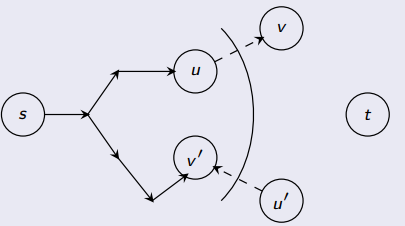
\includegraphics[height=3.5cm]{img/flows/max_flow_proof_res_st_cut1.PNG}
    \caption{The $A$ (left) and $B$ (right) sets in the residual graph along with the examined edges.}
\end{figure}
% ref https://courses.engr.illinois.edu/cs473/fa2010/Lectures/lecture17.pdf
% ref https://people.eecs.berkeley.edu/~nirkhe/cs38notes/maxflow.pdf
% ref https://www.eecs.yorku.ca/course_archive/2003-04/W/3101/flow.pdf
\end{proof}






\subsubsection{Ford Fulkerson Python implementation}
\marginnote{\faCogs\ \ref{app:ffa_code}\ \faCogs}
An implementation of FFA adapted from \TODO[ref] is found in \ref{app:ffa_code}. It builds the network in Table \ref{tab:ffa_step_by_step} and outputs $23$, as found manually.
% ref http://www.cse.unt.edu/~tarau/teaching/AnAlgo/Ford%E2%80%93Fulkerson%20algorithm.pdf

%%%%%%%%%%%%%%%%%%%%%%%%%%%%%%%%
% Max flow
%%%%%%%%%%%%%%%%%%%%%%%%%%%%%%%
% http://www.robots.ox.ac.uk/~az/lectures/opt/lect4.pdf
% http://people.csail.mit.edu/fredo/Classes/Comp_Photo_ENS/slides/09_graphcut.pdf
% https://www-m9.ma.tum.de/foswiki/pub/SS2016/NetworkFlows/network-flows-190416.pdf
% intui: 
% whole: http://jeffe.cs.illinois.edu/teaching/algorithms/notes/23-maxflow.pdf
% intui: http://www.mathcs.emory.edu/~cheung/Courses/323/Syllabus/NetFlow/max-flow-min-cut.html
% proofs: http://www.cs.upc.edu/~mjserna/docencia/grauA/P16/MaxFlow-fib.pdf
% proof: http://www.ifp.illinois.edu/~angelia/ge330fall09_maxflowl20.pdf
% example: https://math.stackexchange.com/questions/2534278/residual-graph-max-flow-intuition-and-correctness
% formal: http://jeffe.cs.illinois.edu/teaching/algorithms/notes/23-maxflow.pdf
% segm appl short: https://theory.stanford.edu/~tim/w16/l/l4.pdf
% bit about penalty function: https://stackoverflow.com/questions/23997801/image-segmentation-with-maxflow
% general seg: http://www.cs.ucf.edu/~bagci/teaching/mic16/lec10.pdf
% exmp https://stackoverflow.com/questions/49956709/algorithm-for-least-cost-image-segmentation
% v good: http://www.math.ucsd.edu/~fan/teach/202/notes/07maxflow15.pdf
% also good: https://ocw.mit.edu/courses/electrical-engineering-and-computer-science/6-046j-design-and-analysis-of-algorithms-spring-2015/lecture-notes/MIT6_046JS15_lec13.pdf
% http://www.es.ele.tue.nl/education/5MC10/9flow.pdf
% https://www.youtube.com/watch?v=XPpmzulEmjA
% https://people.eecs.berkeley.edu/~satishr/cs270/sp13/slides/lec-1.handout-nup.pdf ?
% http://www.cs.princeton.edu/courses/archive/spr05/cos423/lectures/07maxflow.pdf
% http://www.cs.toronto.edu/~vassos/teaching/c73/handouts/max-flow-key-lemma.pdf proof flow lemma
% https://www.cl.cam.ac.uk/teaching/1415/Algorithms/flowcut.pdf flow val lemma proof
% http://courses.csail.mit.edu/6.854/06/scribe/s9-maxflow.pdf flow maths real nice
% http://users.cms.caltech.edu/~umans/cs38/lec11.pdf flow val lemma
% http://www.cs.toronto.edu/~jepson/csc373/lectures/flowValue.pdf
% https://quizlet.com/125825969/cse202-network-flow-flash-cards/
% http://www.cs.toronto.edu/~vassos/teaching/c73/handouts/max-flow-key-lemma.pdf
% http://www.cs.umd.edu/class/fall2017/cmsc451-0101/Lects/lect15-flow-ford-fulk.pdf
% https://inst.eecs.berkeley.edu/~cs170/fa16/lecture-10-13.pdf cut capacity
% http://www.cs.tufts.edu/~cowen/advanced/lect3-final.pdf cut cap example
% https://stackoverflow.com/questions/40277603/is-minimum-cut-same-for-the-graph-after-increasing-edge-capacity-by-1-for-all-ed min cut what if increase caps?
% https://stackoverflow.com/questions/15645462/does-a-given-network-has-a-unique-min-cut uniqueness?
% http://www.cs.umd.edu/class/fall2017/cmsc451-0101/Lects/lect15-flow-ford-fulk.pdf resid network
% http://www.cs.toronto.edu/~lalla/373s16/notes/MFMC.pdf flow cap remove edge
% http://vision.stanford.edu/teaching/cs231a_autumn1112/lecture/lecture6_clustering_and_seg_p2_cs231a_marked.pdf segm n cuts
% http://scikit-image.org/docs/dev/auto_examples/segmentation/plot_ncut.html in scikit
% http://www.maths.lth.se/vision/education/pages/Rykfors12/exjobb.pdf
% http://www.ece.mcmaster.ca/~xwu/703/maxflow.pdf resid fig @sl 9
% https://www.hackerearth.com/practice/algorithms/graphs/maximum-flow/tutorial/ ford fulk example
% https://www.coursera.org/lecture/advanced-algorithms-and-complexity/residual-networks-TIGj4 resid vid
% https://people.cs.umass.edu/~mcgregor/611F17/lec11.pdf resid gud
% https://www.cs.princeton.edu/courses/archive/spring13/cos423/lectures/07DemoFordFulkerson.pdf algo demo
% https://cs.stackexchange.com/questions/55041/residual-graph-in-maximum-flow intui, back edges
% https://stackoverflow.com/questions/19453217/why-are-back-edges-required-in-the-ford-fulkerson-algorithm back edges
% http://www.cs.princeton.edu/courses/archive/spring11/cos226/lectures/21-64MaxFlow.pdf sl 27 back edges
% https://stackoverflow.com/questions/21471043/find-all-edges-in-min-cut verbose expl
% https://courses.engr.illinois.edu/cs473/sp2011/Lectures/17_notes.pdf algo details
% http://people.seas.harvard.edu/~cs125/fall16/section-notes/05.pdf advanced applications
% https://cs.stackexchange.com/questions/55041/residual-graph-in-maximum-flow great example
% https://www.eecs.wsu.edu/~holder/courses/CptS223/spr09/slides/netflow.pdf why bacl edge
% http://ace.cs.ohiou.edu/~razvan/courses/cs4040/lecture21.pdf good exmp and resid graph next to it




\subsection{Normalised Cuts}

\subsubsection{Drawback of classic graph cuts}
% ref https://people.eecs.berkeley.edu/~malik/papers/SM-ncut.pdf
To reiterate the problem studied in the previous section, we want to partition flow network (weighten, directed graph with a source $s$ and sink $t$ and capacities $c$) $G=(V,E,s,t,c)$ into two disjoint vertex sets $A, B, \ A\cup B = V, \ A\cap B = \emptyset$ by simply removing tbe edges connetcting the two sets.\\
The degree of dissimilarity between these two sets can be computed as total weight (capacity)
of the edges that have been removed. This is the $(S,T)$ cut capacity defined in \eqref{eq:def_cut_cap}:
\[
\textup{cut}(A,B)=\sum\limits_{u\in A,\ v\in B}{c\left( u,v \right)}
\]
The optimal bipartitioning of a graph is the one that \textit{minimises this cut value}. In Fig. \ref{fig:classic_bad_cut}, we have a number of nodes and we assume that the edge weights are inversely proportional to the distance between the two nodes. Hence the (imaginary) edges on the right will have smaller weights as the nodes are far away. Attempting a minimum weight cut e.g. by FFA would likely yield the partitions $n1$ or $n2$. We see how the minimum cut criteria favour cutting small sets of isolated nodes in the graph as cut weight defined above increases with the number of edges going across the two partitioned parts.
\begin{figure}[H]
	\centering %centralizar a figura
	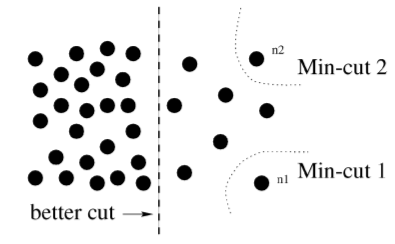
\includegraphics[height=3.75cm]{flows/classic_bad_cut.PNG}
    \caption{A case where minimum cut gives a bad partition}
    \label{fig:classic_bad_cut} % label always after caption!
\end{figure}


% ref https://people.eecs.berkeley.edu/~malik/papers/SM-ncut.pdf



\subsubsection{Normalised Cut Concepts}

To get rid of this bias, we compute the cut between two sets cost as a fraction of the total edge connections to all the nodes in the graph (remember, we want the cut weight to be as small as possible). This weight, called \emphasis{normalised cut} measures the disassociation between  two sets $A,B$ s.t. $A\cup B = V$ and is defined  as
\begin{equation}
    Ncut(A,B) = \frac{c(A,B)}{assoc(A,V)} + \frac{c(A,B)}{assoc(B,V)}
    \label{eq:ncut_def}
\end{equation}
, where
\begin{equation}
    assoc(A,V) = \sum\limits_{u\in A,\ v\in B}{c\left( u,v \right)}
\end{equation}
is the total connection from nodes in $A$ to all nodes in the graph. $Ncut$ or ``disassociation'' between two clusters $A$ and $B$ is a quantity we want to \textit{minimise}. Partition the graph so that edges within a group have large weights and edges across groups have small weights.
\begin{itemize}
    \item If we intuitively think that for two nodes $u\in A,v\in B$, $c(u,v) \propto 1/r(u,v)$, where $r$ is the distance, then the higher the distance between the two sets, the smaller the $c(A,B)$.
    \item At the same time, we want to maximise $assoc(A,V),\ assoc(B,V)$. $assoc(A,V)$ is increased by increasing the number of vertices in $A$.
\end{itemize}
\begin{figure}[H]
	\centering %centralizar a figura
	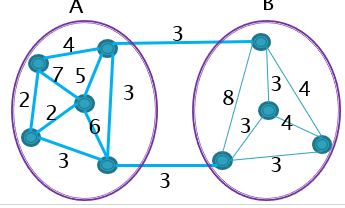
\includegraphics[height=3.15cm]{ncuts/ncuts_2_clusters_numbered.PNG}
    \caption{$assoc(A,V) = 4+7+5+2+2+3+6+3+3+3=38$}
\end{figure}

The figures below how $asso(A,V)$ and $c(A,B)$ can be interpreted graphically.

\begin{multicols}{3}

\begin{figure}[H]
	\centering %centralizar a figura
	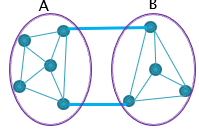
\includegraphics[height=2.75cm]{ncuts/ncuts_2_clusters_cutAB.PNG}
    \caption{$cut(A,B) = \sum\limits_{u\in A,\ v\in B}{c\left( u,v \right)}$}
    %\label{fig:classic_bad_cut} % label always after caption!
\end{figure}
\columnbreak

\begin{figure}[H]
	\centering %centralizar a figura
    	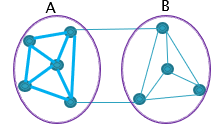
\includegraphics[height=2.75cm]{ncuts/ncuts_2_clusters_asscAA.PNG}
    \caption{$assoc(A,A)= \sum\limits_{u\in A,\ v \in A}{c(u,v)}$}
    %\label{fig:classic_bad_cut} % label always after caption!
\end{figure}
\columnbreak

\begin{figure}[H]
	\centering %centralizar a figura
    	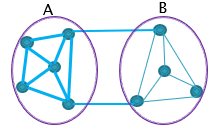
\includegraphics[height=2.75cm]{ncuts/ncuts_2_clusters_asscAV.PNG}
    \caption{$assoc(A,V)= \sum\limits_{u\in A,\ v \in V}{c(u,v)}$}
    %\label{fig:classic_bad_cut} % label always after caption!
\end{figure}
\end{multicols}
From the diagrams, we can see that
\begin{equation}
    assoc(A,V) = assoc(A,A) + cut(A,B), \ \ A\cup B = V
    \label{eq:assoc_wrt_cut}
\end{equation}

Figure below demonstrates the definitions in \eqref{eq:ncut_def}, \eqref{eq:assoc_wrt_cut}.
\begin{figure}[H]
	\centering %centralizar a figura
    	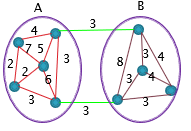
\includegraphics[height=2.75cm]{ncuts/ncuts_2_clusters_num_col.PNG}
    \caption{$Ncut(A,B) = 
    \frac{\textcolor{green}{6}}
    {\textcolor{green}{6}+\textcolor{red}{29} } +
    \frac{\textcolor{green}{6}}
    {\textcolor{green}{6}+\textcolor{brown}{29}}$
    }
    %\label{fig:classic_bad_cut} % label always after caption!
\end{figure}
We can define the \emphasis{normalised association} for two sets $A,B$ s.t. $A \cap B = V$ in a similar way with normalised cut:
\begin{equation}
    Nassoc(A,B) = \frac{assoc(A,A)}{assoc(A,V)} +\frac{assoc(B,B)}{assoc(B,V)}  
    \label{eq:nassoc_def}
\end{equation}
Using \eqref{eq:assoc_wrt_cut}:
\begin{equation}
    Nassoc(A,B) = 
    \frac{\textcolor{red}{assoc(A,A)}}{\textcolor{red}{assoc(A,A)} + \textcolor{green}{cut(A,B)}} + 
    \frac{\textcolor{brown}{assoc(B,B)}}{\textcolor{brown}{assoc(B,B)} + \textcolor{green}{cut(A,B)}} 
    \label{eq:nassoc_wrt_cut}
\end{equation}
\begin{figure}[H]
	\centering %centralizar a figura
    	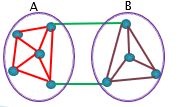
\includegraphics[height=2.75cm]{ncuts/ncuts_2_clusters_asso_ext.PNG}
    \caption{Illustration of normalised association as derived in \ref{eq:nassoc_wrt_cut}}
    %\label{fig:classic_bad_cut} % label always after caption!
\end{figure}
Using the definition of normalised cut (\eqref{eq:ncut_def}) and \eqref{eq:nassoc_wrt_cut} we can express the former as a function of normalised association:
\begin{equation}
    Ncut(A,B) = \frac{assoc(A,V) - assoc(A,A) }{assoc(A,V)} + \frac{assoc(B,V) - assoc(B,B) }{assoc(B,V)} = 2 - Nassoc(A,B)
\end{equation}
% par ref http://www.dccia.ua.es/~sco/Spectral/Lesson3_Cuts.pdf
Therefore to minimise $Ncut(A,B)$ we want to maximise $Nassoc(A,B)$. $Nasso$ is encodes the association within the group, i.e. the ratio between how many weight remains inside over what goes outside for both groups.




\subsubsection{From Undirected Graphs to Matrices}
Deriving the clustering that minimizes these objective functions is NP-hard but can be solved by a relaxation. We use spectral graph theroy for that purpose. 
\begin{definition}
For an undirected weighted graph, let \textbf{W} be a matrix where $W_{i,j}$ denotes the weight of the edge $e(i,j)$:
\end{definition}
Because $w_{i,j} = w_{j,i}$, \textbf{W} is \textit{real and symmetric}.
\begin{definition}
For an undirected weighted graph, let $\textbf{D}$ be a diagonal matrix where $D_{i,i}$ denotes the sum of the weights of the edges $e(i,j)$ for every other node $j$:
\end{definition}
\begin{corollary}
By definition of the $\textbf{D}$ and $\textbf{W}$ matrices,
\[
{{d}_{ii}}=\sum\limits_{j=1}^{N=\#vert}{{{w}_{ij}}}
\]
\end{corollary}
For example, for the graph below, 
\begin{figure}[H]
	\centering %centralizar a figura
    	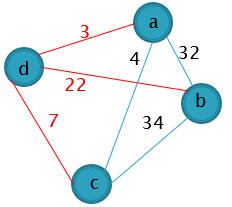
\includegraphics[height=3.25cm]{ncuts/graph_1_cluster.PNG}
    \caption{Sample undirected graph with 1 connected component (1 connected cluster)}
    \label{fig:undir_graph_1_cluster}
    %\label{fig:classic_bad_cut} % label always after caption!
\end{figure}
\[
\textbf{W} = \begin{bmatrix}
0 & 32& 4& 3\\
32 & 0 &34 & 22&\\
4& 34& 0 &7\\
3& 22& 7& 0
\end{bmatrix},\
\textbf{D} = 
\begin{bmatrix}
39 & 0& 0& 0\\
0& 88 &0 & 0&\\
0& 0& 45 &0\\
0& 0& 0& 32
\end{bmatrix}
\]
We also define the Laplacian matrix in terms of $\textbf{W}$ and $\textbf{D}$ - this tells us things about the connectivity of the graph such as the number of spanning trees for a given graph.
\begin{definition}
For an undirected weighted graph, let \textbf{L} (\emphasis{Laplacian}) be a matrix where $\textbf{L} = \textbf{D}-\textbf{W}$:
\end{definition}
For example, for the graph in Fig. \ref{fig:undir_graph_1_cluster} given the $\textbf{W}$ and $\textbf{D}$ matrices we have found, we can compute the Laplacian as
\[
\textbf{L} = \textbf{D}-\textbf{W} = \begin{bmatrix}
39 & 0& 0& 0\\
0& 88 &0 & 0&\\
0& 0& 45 &0\\
0& 0& 0& 32
\end{bmatrix}
- 
\begin{bmatrix}
0 & 32& 4& 3\\
32 & 0 &34 & 22&\\
4& 34& 0 &7\\
3& 22& 7& 0
\end{bmatrix}
=
\begin{bmatrix}
39 & -32& -4& -3\\
-32& 88 &-34 & -22&\\
-4& -34& 45 &-7\\
-3& -22& -7& 32
\end{bmatrix}
\]
$\textbf{L}$ has a number of useful properties.
\begin{corollary}\quad \\
\begin{enumerate}
    \item The Laplacian matrix is real and symmetric.
    \item Therefore All its eigenvectors are perpendicular to each other.
    \item It is positive semi-definite, i.e. $\textbf{x}_{m\times 1}^T \textbf{L}_{m \times n}\textbf{x}_{m\times 1}\geq \textbf{0} \ \ \forall \textbf{x}  \neq \textbf{0}$
    \item Therefore all its eigenvalues are non-negative (proof of this is beyond the scope) and $0 \leq \lambda_1 \leq ... \leq \lambda_n$.
    \item It has at least one zero eigenvalue.
\end{enumerate}
\end{corollary}
\begin{proof} (Property 5)\\
When we have a connected component (a connected subgraph of the original graph), for each row of $\textbf{L}_{m \times n}$, for diagonal element of the Laplacian we have 
\[
{{L}_{ii}}=-\sum\limits_{j=1,\ j\ne i}^{n}{{{L}_{ij}}}
\]
For example, for our $L$ matrix in \ref{fig:undir_graph_1_cluster}, the weight leaving node $a=39=32+4+3=w_{a,b} + w_{a,c} + w_{a,d}$ or in terms  of the Laplacian:
\[
\begin{split}
    L_{11} &= -L_{12} -L_{13} -L_{14} \Leftrightarrow 39 = -(-32-4-3)\\
    L_{21} &= -L_{22} -L_{23} -L_{24} \Leftrightarrow 88 = -(-32- 34-22)\\
    L_{31} &= -L_{32} -L_{33} -L_{34} \Leftrightarrow 45=-(-4-34-7)\\
    L_{41} &= -L_{42} -L_{43} -L_{44} \Leftrightarrow 32=-(-3-22-7)\\
\end{split}
\]
Writing the \TODO[number them] in terms of dot product we have:
\[
\begin{aligned}[c]
    L_{11}\cdot 1 +L_{12}\cdot 1 +L_{13}\cdot 1 +L_{14}\cdot 1=0\\
    L_{21}\cdot 1 +L_{22}\cdot 1 +L_{23}\cdot 1 +L_{24}\cdot 1=0\\
    L_{31}\cdot 1 +L_{32}\cdot 1 +L_{33}\cdot 1 +L_{34}\cdot 1=0\\
    L_{41}\cdot 1 +L_{42}\cdot 1 +L_{43}\cdot 1 +L_{44}\cdot 1=0\\
\end{aligned}
\quad \Leftrightarrow \quad
\begin{aligned}[c]
    \myunderbrace{
    \begin{bmatrix}
        \textbf{L}_{1:}\\
        \textbf{L}_{2:}\\
        \textbf{L}_{3:}\\
        \textbf{L}_{4:}
    \end{bmatrix}
    }
    {\textbf{L}}
    \myunderbrace{
    \begin{bmatrix}
        1\\1\\1\\1
    \end{bmatrix}
    }{\textbf{x}}
    =
    \begin{bmatrix}
        0\\0\\0\\0
    \end{bmatrix}
    = \myunderbrace{\ 0\ }{\lambda} \cdot 
    \myunderbrace{
    \begin{bmatrix}
        1\\1\\1\\1
    \end{bmatrix}
    }
    {\textbf{x}}
\end{aligned}
\]
Therefore a connected component yields a zero eigenvalue. 
\end{proof}
Furthermore, the number of ones in its eigenvector is equal to the number of connected nodes in it. To verify that, consider the following graph which contains two connected components.
\begin{figure}[H]
	\centering %centralizar a figura
    	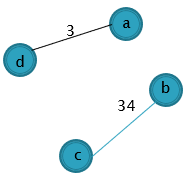
\includegraphics[height=3.25cm]{ncuts/graph_2_cluster.PNG}
    \caption{Sample undirected graph with 2 connected components.}
\end{figure}
For this 2-component graph, we have the following matrices:
\[
\textbf{W} = 
\begin{bmatrix}
0 & 0& 0& 3\\
0 & 0& 34& 0\\
0 & 34& 0& 0\\
3 & 0& 0& 0
\end{bmatrix}
,\
\textbf{D }= 
\begin{bmatrix}
3 & 0& 0& 0\\
0 & 34& 0& 0\\
0 & 0& 34& 0\\
0 & 0& 0& 3
\end{bmatrix}
,\
\textbf{L}=
\begin{bmatrix}
3 & 0& 0& -3\\
0 & 34& -34& 0\\
0 & -34& 34& 0\\
-3 & 0& 0& 3
\end{bmatrix}
\]
% ref detailed proof: http://math.uchicago.edu/~may/REU2013/REUPapers/Marsden.pdf
For the eigen-data of $\textbf{L}$ we have:
\[
\begin{split}
\textbf{L}\cdot 
\begin{bmatrix}
1\\0\\0\\1
\end{bmatrix}=
\begin{bmatrix}
3 & 0& 0& -3\\
0 & 34& -34& 0\\
0 & -34& 34& 0\\
-3 & 0& 0& 3
\end{bmatrix}
\cdot
\begin{bmatrix}
1\\0\\0\\1
\end{bmatrix}=
\begin{bmatrix}
0\\0\\0\\0
\end{bmatrix}
=
0 \cdot 
\begin{bmatrix}
1\\1\\1\\1
\end{bmatrix}
\\
\textbf{L}\cdot 
\begin{bmatrix}
0\\1\\1\\0
\end{bmatrix}=
\begin{bmatrix}
3 & 0& 0& -3\\
0 & 34& -34& 0\\
0 & -34& 34& 0\\
-3 & 0& 0& 3
\end{bmatrix}
\cdot
\begin{bmatrix}
0\\1\\1\\0
\end{bmatrix}=
0 \cdot 
\begin{bmatrix}
1\\1\\1\\1
\end{bmatrix}
\end{split}
\]
\begin{corollary}
The number of connected component in an undirected graph equals the multiplicity eigenvalues of the Laplacian matrix \textbf{L}.
\end{corollary}
\begin{definition}
The smallest non-zero eigenvalue of \textbf{L} is called the \emphasis{spectral gap} (we will use this eigenvalue).
\end{definition}
% ref https://arxiv.org/pdf/1311.2492.pdf
In general, the spectrum $(0,\lambda_2, \ldots , \lambda_m)$ contains a lot of information about the combinatorial structure of the graph but this is not a subject of study of this article. More information can be found at \TODO[ref].




\subsubsection{Solving the Ncut Problem}

The definitions of $\textbf{W},\ \textbf{D},\ \textbf{L}$ are useful because they can transform the Ncut problem in a more concrete optimisation one. Recall the definition of $Ncut$ in \eqref{eq:ncut_def}. If we also definie a \emphasis{selector vector} $\textbf{x}$ that tells us whether a vertex belongs in cut set $A$ ($A\cup B = V, \ m = \left|V \right|$) as
%ref http://www.dccia.ua.es/~sco/Spectral/Lesson3_Cuts.pdf
\begin{equation}
    \textbf{x} \in \mathbb{R}^m: \ \ x_{i} = 
    \left\{
\begin{array}{ll}
      1, \; \; &v_i \in A\\
      -1, \; \; &v_i \notin A
\end{array} 
\right. 
\end{equation}
Then for the edges $(i,j)$ that belong in the cut, e.g. $x_i\in A,\ x_j\in B$ we have $x_i=1, \ x_j=-1 \Rightarrow w_{ij} = - w_{ij}x_ix_j$ so
\begin{align}
    Ncut(A,B) &= \frac{cut(A,B)}{assoc(A,V)} + \frac{cut(A,B)}{assoc(B,V)} \nonumber \\
    &= \frac{\sum\limits_{{{x}_{i}}> 0,\ {{x}_{i}}< 0}{-{{w}_{ij}}{{x}_{i}}{{x}_{j}}}}{\sum\limits_{{{x}_{i}}> 0}{{{d}_{i}}}}
    +
    \frac{\sum\limits_{{{x}_{i}}< 0,\ {{x}_{i}}> 0}{-{{w}_{ij}}{{x}_{i}}{{x}_{j}}}}{\sum\limits_{{{x}_{i}}< 0}{{{d}_{i}}}}
\end{align}
Defining $k=\tfrac{\sum\limits_{{{x}_{i}}> 0}{{{d}_{i}}}}{\sum\limits_{{{i}_{}}}{{{d}_{i}}}}$, $b=\tfrac{k}{1-k}=\tfrac{\sum\limits_{{{x}_{i}}> 0}{{{d}_{i}}}}{\sum\limits_{{{x}_{i}<0}}{{{d}_{i}}}}$, $\textbf{y}=(\textbf{1}+\textbf{x}) -b(\textbf{1}-\textbf{x})$ % ref same as above https://people.eecs.berkeley.edu/~malik/papers/SM-ncut.pdf
\TODO[ref] and also observing \TODO[ref] the following two relationships.

\begin{align}
\textbf{y}^T\textbf{D1}=0\tag{1} \\
\textbf{y}^T\textbf{Dy}=b\textbf{1}^T\textbf{D1} \tag{2}
\end{align}

The minimisation problem is transformed to
\[
\underset{\mathbf{x}}{\mathop{\min }}\,Ncut\left( \mathbf{x} \right)=\underset{\mathbf{y}}{\mathop{\min }}\,\frac{{{\mathbf{y}}^{T}}\left( \mathbf{D}-\mathbf{W} \right)\mathbf{y}}{{{\mathbf{y}}^{T}}\mathbf{Dy}} \tag{3}
\]
given the condition
\[
x_i\in \{-1,1\} \Rightarrow y_i\in \{1,-b \}\tag{4}
\]
% ref quad form: https://math.stackexchange.com/questions/2122051/quadratic-form-in-summation-form
% ref proof
This is again NP-hard but if we relax condition (4) and let $\textbf{y}\in \mathbb{R}^m$. Details on the proof are found in \TODO[ref] but we can derive some intuitive results about how $\textbf{y}$ should look like.\\
We want to minimise the numerator in (3), which is:
\begin{align}{c}
\textbf{y}^T\textbf{Dy} - \textbf{y}^T\textbf{Wy} =  \tag{5} \\ 
\sum\limits_{i}{d_{ii}y_i^2} - \sum\limits_j \sum\limits_i{w_{ij}y_iy_j} = \tag{6} \\
\frac{1}{2}\sum\limits_{i}{\left( \sum\limits_{j}{{{w}_{ij}}} \right)}y_{i}^{2} - 
\sum\limits_j \sum\limits_i{w_{ij}y_iy_j}
+\frac{1}{2}\sum\limits_{i}{\left( \sum\limits_{i}{{{w}_{ij}}} \right)}y_{i}^{2}=\tag{7} \\
\frac{1}{2}\left( \sum\limits_{i}{ \sum\limits_{j}{{{w}_{ij}}} }y_{i}^{2} - 
2\sum\limits_j \sum\limits_i{w_{ij}y_iy_j}
+\sum\limits_{i}{ \sum\limits_{i}{{{w}_{ij}}} }y_{i}^{2}\right) =\tag{8} \\
\sum\limits_{ij}w_{ij}\left(y_i - y_j \right)^2 \geq 0 \tag{9}
\end{align}
We transit from (5) to (6) by expanding the quadratic form \TODO[ref].Therefore to minimise the Ncut we want $y_i,y_j,\ i\neq j$ to be as close as possible and $w_{ij}$ to be as small as possible, but we care less about $w_{ij}$.
\TODO[ref] prove that we can find the optimal selector vector $\textbf{y}$ by solving the eigensystem
\begin{equation}
    (\textbf{D}-\textbf{W})\textbf{y}=\lambda \textbf{Dy}
\end{equation}
for the second smallest eigenvector $\textbf{y}_2$
\begin{equation}
    \textbf{y}_2 = \textup{arg}\ \underset{{{\mathbf{y}}^{T}}\mathbf{D1}=0}{\mathop{\min }}\,\frac{{{\mathbf{y}}^{T}}\left( \mathbf{D}-\mathbf{W} \right)\mathbf{y}}{{{\mathbf{y}}^{T}}\mathbf{Dy}}
\end{equation}
%REF http://phdfb1.free.fr/phdthesis/node108.html
The solution $\textbf{y}_2$ of the relaxed problem can be used as an approximate solution to the original discrete problem. To "discretise" it, we need to choose a threshold, forcing $\textbf{y}_2$ to take two values, let's say $a$ and $b$. These values separate the vertices in two sets $A$ and $B$.
\begin{figure}[H]
	\centering %centralizar a figura
    	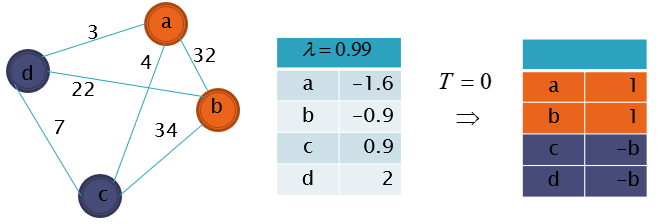
\includegraphics[height=3.25cm]{ncuts/graph_num_cut_eigen.PNG}
    \caption{Partitioning the graph using the relaxed condition $y_i\in \mathbb{R} $ threshold $T=0$ for the selector vector.}
\end{figure}


\subsubsection{$Ncut$ in More Than 2 Partitions}
% ref https://www.cs.cmu.edu/~aarti/Class/10701/slides/Lecture21_2.pdf
To split in further partitions

recursive 2-way cut:
Given G=(V,E)  compute matrixes D and W
% ref Presented To: Prof. Hagit Hel-Or Presented by: Avner And David
% REF https://www.ijcsmc.com/docs/papers/April2013/V2I4201371.pdf 303

Compute for eigenvector with the second smallest eigenvalue and perform bi-partition of the graph.

Stopping condition:
Check stability of eigenvector values- see if the values are continues.
$N_{cut} < T$  - where $T$ is a predefined value to indicate if the $N_{cut}$ should be stopped.


% asso and ncut exmp
% http://www.dccia.ua.es/~sco/Spectral/Lesson3_Cuts.pdf
% http://digitalassets.lib.berkeley.edu/techreports/ucb/text/CSD-97-940.pdf
% http://www.dccia.ua.es/~sco/Spectral/Lesson3_Cuts.pdf




\subsubsection{Transforming Images into Graphs}

% ref superpix http://www.kev-smith.com/papers/SLIC_Superpixels.pdf
Before attempting to transform images into graph, we cluster together pixels with similar properties into \emphasis{superpixels} using techniques such as SLIC, described in \TODO[ref]. The image, converted into a set of superpixels can be transformed into a graph. Each node represents a superpixel and the weight $w_i{ij}$ between nodes $(v_i,v_j)$ depends on their distance and feature similarity (e.g. intensity or RBG difference). A common way to defined those edge weights is
% ref http://www-users.cselabs.umn.edu/classes/Spring-2017/csci8314/Talks/bo-slides.pdf
\begin{equation}
    w_{ij}= \exp\left(-\tfrac{\left|\left|\textbf{F}_i - \textbf{F}_j \right|\right|)_2^2}{\sigma_F^2}\right) \cdot \left\{
\begin{array}{ll}
      \exp\left(-\tfrac{\left|\left|\textbf{X}_i - \textbf{X}_j \right|\right|)_2^2}{\sigma_X^2}\right) &,\ \left|\left|\textbf{X}_i - \textbf{X}_j \right|\right| < r\\ 
      0 &,\ \textup{otherwise}
\end{array} 
\right.
\end{equation}
$\textbf{F}_i$ is the feature value of node $v_i$, e.g. the intensity or RBG value and $\textbf{X}_i$ the spatial location of its centre.



\subsubsection{Implementing $Ncut$}

\mintinline{latex}{scikit-image} provides an API to implement segmentation by normalised cuts. Segmentation is not applied directly on an RGB - it follows some steps.
% API ref http://scikit-image.org/docs/dev/api/skimage.future.graph.html#skimage.future.graph.cut_normalized
\begin{enumerate}
    % ref  http://www.kev-smith.com/papers/SLIC_Superpixels.pdf
    \item (\mintinline{python}{skimage.segmentation.slic()}) Combine the image pixels into \emphasis{superpixels} by using the SLIC superpixel method \TODO[ref]. SLIC superpixels is itself another segmentation method that uses k-means to group together nearly pixels into cube-like segments. The grouping criterion depends on the space and colour proximity. Output a labelled image.
    \item (\mintinline{python}{skimage.future.graph.rag_mean_color()}) Construct the \emphasis{region adjacency graph} (RAG) of the superpixel labelled image. Each node in the RAG represents a set of pixels within image with the same label in labels. The weight between two adjacent regions represents how similar or dissimilar two regions are depending on their mode parameter (distance or intensity difference). 
    \item (\mintinline{python}{skimage.future.graph.cut_normalized()}) Perform normalised cuts on the RAG. It needs the labelled superpixel image \textit{and} the RAG and utilises a default threshold to stop subdiving the graph and a default number of cuts. 
\end{enumerate}
\marginnote{\faCogs \ref{app:ncuts_code}\faCogs}
The code, adapted from \mintinline{latex}{scikit-image}'s documentation, is listed in \ref{app:ncuts_code} and the results from each step are shown below.
\begin{figure}[H]
	\centering %centralizar a figura
    	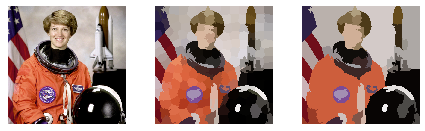
\includegraphics[height=3.25cm]{ncuts/scikit-ncut.png}
    \caption{Results of the Ncut \mintinline{latex}{scikit} code.Left: original , middle: step (1), right: step (3).}
\end{figure}


\subsection{Grab Cut}

\subsubsection{Grab cut overview}
% ref https://cvg.ethz.ch/teaching/cvl/2012/grabcut-siggraph04.pdf
Grab \TODO[ref] cut is a powerful algorithm that treats the image as a foreground-background graph and also relies on energy function minimisation. It includes the following features:
\begin{itemize}
    \item A powerful, iterative version of energy optimisation based on probabilistic models that encourages border coherence. It is tuned using three coefficients $\alpha,\ \beta,\ \gamma$ in a similar fashion with active contours. However, these coefficents tune quantities more complex than those of the active contours.
    \item It requires some basic user interaction - particularly a bounding box around the object of interest. The rest is taken care of by the algorithm
    \item Border matching and re-learning using probabilistic models to estimate the outline and the colours of the foreground object.
\end{itemize}
% ref https://pdfs.semanticscholar.org/9246/cbf8d7a489b2c6299317416c7dfdf747f72b.pdf
Grab Cut following these higher level steps \TODO[ref]:
\begin{itemize}
    \item User creates an initial trimap by \textit{selecting a rectangle}. Pixels inside the rectangle are marked as unknown. Pixels outside of rectangle are marked as known background.
    \item Computer creates an \textit{initial image segmentation}, where all unknown pixels are tentatively placed in the foreground class
and all known background pixels are placed in the background
class.
    \item \textit{Gaussian Mixture Models} (GMMs) are created for initial foreground and background classes.
    \item Each pixel in the foreground class is \textit{assigned to the most
likely Gaussian component} in the foreground GMM. Similarly, each pixel in the background is assigned to the most
likely background Gaussian component.
    \item  The GMMs are thrown away and \textit{new GMMs} are learned from
the pixel sets created in the previous set.
    \item A graph is built and Graph Cut is run to find a \textit{new tentative
foreground and background} classification of pixels.
    \item Steps 4-6 are repeated until the classification converges.
\end{itemize}
% sources:
% https://cvg.ethz.ch/teaching/cvl/2012/grabcut-siggraph04.pdf
% http://www.maths.lth.se/matematiklth/personal/petter/rapporter/grabcut.pdf
% https://pdfs.semanticscholar.org/9246/cbf8d7a489b2c6299317416c7dfdf747f72b.pdf
% https://grabcut.weebly.com/background--algorithm.html


\subsubsection{Algorithm details}

Before we present the quantities that grab cut deals with, the notation is in the paper presented:
\begin{itemize}
    \item $N$: number of pixels.
    \item $\textbf{a}=[a_1,\ldots,a_N],\ a_n \in \{0,1\}, \ n=1,\ldots,N$: whether a pixel belongs in the background (0) or foreground (1).
    \item $K$: number of GMM's.
    \item $\textbf{k}=\{k_1,\ldots,k_N],\ k_n \in \{1,\ldots,K\}, \ n=1,\ldots,N$.
    \item $\textbf{z}=\{\textbf{z}_1,\ldots,\textbf{z}_N],$ the colour of each pixel.
    \item $\theta$: these parameters describe foreground and background grey-level distributions, and consist of histograms of grey values:
    \[
    \boldsymbol{\theta} = \{h(\textbf{z};\alpha, \ \alpha=\{0,1\} \}
    \]
    one for background ($T_B$) and one for foreground ($T_F$).
\end{itemize}
The segmentation task is to infer the unknown opacity variables
$\alpha$ from the given image data $\textbf{z}$ and the model $\boldsymbol{\theta}$.\\
The energy function to minimise is defined in such a way that it tends to ``solidify'' objects, and is a form of Gibbs energy:
\begin{equation}
    E(\boldsymbol{\alpha}, \textbf{k}, \boldsymbol{\theta}, \textbf{z}) = U(\boldsymbol{\alpha}, \textbf{k}, \boldsymbol{\theta}, \textbf{z}) +V(\boldsymbol{\alpha}, \textbf{z})
\end{equation}
The \textit{data term }$U$ evaluates the fit of the binary distribution $\boldsymbol{\alpha}$ to the
data \textbf{z}, and $V$ is the smoothness term between neighbouring pixels. These are defined as:
\begin{equation}
    U(\boldsymbol{\alpha}, \textbf{k}, \boldsymbol{\theta}, \textbf{z}) =
    \sum\limits_{n}{D(\alpha_n, k_n,\boldsymbol{\theta},z_n)}
\end{equation}
, where:
\[
D(\alpha_n, k_n,\boldsymbol{\theta},z_n) = -\log\, p\left(z_n \left|\alpha_n,k_n,\textbf{z}_n \right. \right) -\log\, \pi (\alpha_n, k_n)
\]
$p(\cdot)$ is a Gaussian probability distribution, and $\pi(\cdot)$ are mixture weighting coefficients.
The \textit{smoothness term} $V$ is defined as:
\begin{equation}
    V(\boldsymbol{\alpha},\textbf{z}) = \gamma \sum\limits_{(m,n) \in \textbf{C}}[\alpha_m \neq \alpha_n] \exp -\beta \left|\left|\textbf{z}_m - \textbf{z}_n \right|\right|^2
\end{equation}
, where $m, n$ are the indexes of two pixels and $\textbf{C}$ is the set of pairs of neighbouring pixels. Constants $\beta, \gamma$ are fixed and chosen as explained in the paper. Given that insight, the Grab Cut algorithm is as follows.
\begin{figure}
    \centering
    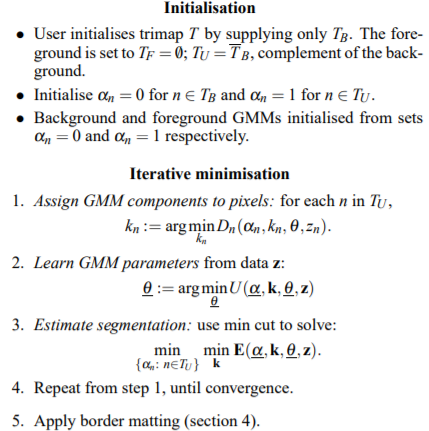
\includegraphics[height=7.5cm]{grabcut/grabcut_algo.PNG}
    \caption{Grab Cut algorithm from Rother et al's paper.}
\end{figure}

\subsubsection{Implementation in OpenCV}

From OpenCV's documentation, function \mintinline{python}{cv.grabCut} takes the following inputs and returns simply the output image. Note that to fine the result \mintinline{python}{grabCut} might have to be run multiple times to refine the output.
\begin{itemize}
    \item \mintinline{python}{img} - Input image,
    \item \mintinline{python}{mask} - It is a mask image where we specify which areas are background, foreground or probable background/foreground etc. It is done by the following flags, \mintinline{python}{cv.GC_BGD}, \mintinline{python}{cv.GC_FGD}, \mintinline{python}{cv.GC_PR_BGD}, \mintinline{python}{cv.GC_PR_FGD}, or simply pass 0,1,2,3 to image.
    \item \mintinline{python}{rect} - It is the coordinates of a rectangle which includes the foreground object in the format \mintinline{python}{(x,y,w,h)}.
    \item \mintinline{python}{bdgModel}, \mintinline{python}{fgdModel} - These are arrays used by the algorithm internally. You just create two \mintinline{python}{np.float64} type zero arrays of size \mintinline{python}{(1,65)}.
    \item \mintinline{python}{iterCount} - Number of iterations the algorithm should run.
mode - It should be \mintinline{python}{cv.GC_INIT_WITH_RECT} or \mintinline{python}{cv.GC_INIT_WITH_MASK} or combined which decides whether we are drawing rectangle or final touchup strokes.
\end{itemize}
OpenCV provides a ready to run example in \mintinline{python}{<root_dir>/samples/python/grabcut.py}.
A result by using the rectangle tool and some fine tuning with the brushes that select one of the \mintinline{python}{cv.GC_BGD}, \mintinline{python}{cv.GC_FGD}, \mintinline{python}{cv.GC_PR_BGD}, \mintinline{python}{cv.GC_PR_FGD} flags is shown below.
\begin{multicols}{2}
\begin{figure}[H]
    \centering
    \includegraphics[height=4cm]{img/grabcut/grabcut_input.PNG}
    \caption{Grab cut input}
\end{figure}
\columnbreak
\begin{figure}[H]
    \centering
    \includegraphics[height=4cm]{img/grabcut/grabcut_output.PNG}
    \caption{Grab cut output after rectangle selection and some fine turning using the masks.}
\end{figure}
\end{multicols}




\subsubsection{Grab cut pros and cons}

\begin{multicols}{2}
    \begin{itemize}
        \item[\textcolor{DarkPink}{\ding{51}}] Extracts the object very accurately and unsusceptible to noise, boundary discontinuities etc.
        \item[\textcolor{DarkPink}{\ding{51}}] Can be modified for better and better result.
    \end{itemize}
    
    \columnbreak
    \begin{itemize}
        \item[\textcolor{DarkPink}{\ding{55}}] Too slow to be used in real time.
        \item[\textcolor{DarkPink}{\ding{55}}] Not always easy to correctly extract the object without user input.
        
    \end{itemize}
\end{multicols}










\section{Watershed method}


\subsection{Watershed by Immersion Segmentation}

\subsubsection{Parallelism with geography and concepts}

The watershed method treats a digital image ($f: \mathbb{Z}^2 \rightarrow \mathbb{Z}$) as a topological surface. Particularly, it treats the image intesnity as altitude, so low intensity regions yield valleys and high intensity regions ridges. Because the watershed method assumes that we pour water on the image, valleys are also called ``catchment basins''. The watershed often results in \textit{oversegmentation} and we will describe how to control this.\\
% ref http://www.cmm.mines-paristech.fr/~beucher/wtshed.html
In fact, the watershed is not applied to the image itself but to the \textit{gradient}, so that the ``catchment basins'' theoretically correspond to the homogeneous grey level regions of the image.
\begin{definition}
in geography, a \emphasis{watershed} is a ridge that divides areas drained by different river systems. 
\end{definition}
\begin{definition}
A \emphasis{Catchment basin} is the geographical area draining into a river or a reservoir
\end{definition}
\begin{definition}
\emphasis{Ridge lines/ watershed lines} are the points at which the water is equally likely to fall to more than one minimum.
\end{definition}
% red ^https://www.coursera.org/lecture/digital/watersheds-and-k-means-algorithms-KHf3u

% ref https://imagej.net/_images/c/c5/Watershed-flooding-graph.png
\begin{figure}[H]
	\centering %centralizar a figura
    	\includegraphics[height=3.0cm]{watershed/wateshed_sample_defs.png}
    \caption{The catchment basin and watershed lines (ridges) of a sample greyscale image.}
\end{figure}
In the watershed transforrm there are 3 types of points
\begin{enumerate}
    \item Points belonging to a \emphasis{regional minimum}.
    \item \emphasis{Catchment basis} of a regional minimum - points at which a drop of water will certainly fall to single minimum.
    \item \emphasis{Ridge lines/ watershed lines} - points at which a drop of water will be equally likely to fall to more than one minimum.
\end{enumerate}
% ref https://hal.inria.fr/hal-01113462/document
The drop of water principle, watersheds and how they are related from the perspective of graphs are rigorously explained here \TODO[ref]. 




\subsubsection{The watershed algorithm - overview}

\faQuestionCircle \ What is the \textit{goal} of watershed?\\
\faCheckCircle \ The goal of watershed is to find the watershed lines. This is done by a technique called immersion by contructing dams between two watersheds that are about to merge. \\
\faQuestionCircle \ What is the \textit{process} of watershed?\\
\faCheckCircle \ 
% ref https://www.uio.no/studier/emner/matnat/ifi/INF4300/h11/undervisningsmateriale/INF4300-2011-f04-segmentation.pdf
    We interpret the image as a 3D topographic surface ($x\ ,y,\ $intensity), with both valleys and mountains.
\begin{enumerate}
    \item (\textit{holes at minima}) Find all local minima. Punch a tiny hole in each one of them.
    \item (\textit{immersion step})Slowly immerse the topographic surface into a lake so the water rises through the holes so the water rises through the local minima across the entire image at uniform rate.
    \item (\textit{dam construction step}) When rising water in distinct catchment basins is about to merge, a dam is built to prevent merging.
    \item (\textit{watershed extraction step})Final step: the only thing visible would be the dams. The connected dam boundaries correspond to the watershed lines.
\end{enumerate}


 
 \begin{figure}[H]
	\centering %centralizar a figura
    	\includegraphics[height=4.75cm]{watershed/watershed_1d_toy_example.png}
    \caption{The catchment basin and watershed lines (ridges) of a sample greyscale image.}
\end{figure}
 
 
 Figure \ref{fig:wshed_matrix_example} illustrates the intuition behind steps (1)-(4). The next two sections attempt to answer how exactly dams are constructed and the flooding mechanism. 

\begin{figure}[H]
    % ref http://www.cs.rug.nl/~roe/courses/ip/10_segment-handout.pdf}
    \centering
    \includegraphics[scale=0.835]{watershed/watershed_matrix_example.PNG}
    \caption{Watershed flooding on a matrix. It starts from the three local minima of $0$.}
    \label{fig:wshed_matrix_example}
\end{figure}
 
 
 
 
 \subsubsection{The watershed algorithm - finding the watershed lines}
 
 
 \faQuestionCircle \ \textit{How} is the dam constructed (step 3)?\\
 \faCheckCircle \ 
 % dilation ref https://www.uio.no/studier/emner/matnat/ifi/INF2310/v17/undervisningsmateriale/slides_inf2310_s17_week15.pdf
 \mycomment{This answer does not explain when the dam it built, but how. When it is built is based on the flooding step and will be discussed later.}
It is constucted based on the \textit{morphological dilation} of the catchment basins. The dilation is not made on the gradient image itself but on a binary image. At each step of the algorithm, the binary
image in obtained in the following
manner.
\begin{enumerate}
    \item Initially, the set of pixels with minimum grey level are 1, others 0.
    \item In each subsequent step, we flood the 3D
topography from below and the pixels
covered by the rising water are ones (black in Fig. \ref{fig:bw_illustration_cb}) and
others zeros (white in the same Figure).
\end{enumerate}
We define the following.
\begin{itemize}
    \item $M_1, \ M_2$ - Sets of coordinates of points around the regional minima, i.e. points around them that have the same height as the minima.
    \item $C_{n-1}(M_1), \ C_{n-1}(M_2)$ - sets of coordinates of points in the catchment basins associated with $M_1,\ M_2$ at stage $n-1$ of flooding (points from minimum of basin to flooding level).
    \item $C[n-1]:=C_{n-1}(M_1) \cup C_{n-1}(M_2)$
\end{itemize}
 The dam is constructed in the following situation. Assume we increase the water by one. At flooding step  $n-1$, there are two connected components (CC). At
flooding step $n$, there is only one connected component, therefore there is a plateau between CC1 and CC2 that allowed them them to flood. The water between the two catchment basins has merged at flooding step $n$. Use $q$ to denote the single connected component. $q$ practically encompasses $C_{n-1}(M_1),\ C_{n-1}(M_2)$ and the flat area around them. \\
Dilation by a $3\times 3$ matrix of ones is performed repeatedly on the catchment basins as they were at step $n-1$. Dilation is constrained on CC $q$, i.e. it (essentially the centre of the dilation mask matrix) cannot go beyond the plateau around catchment basins $C_{n-1}(M_1),\ C_{n-1}(M_2)$. Dilation stops when the dilated CC's get merged.\\
The dam is constructed by
the points on which the
dilation would cause the
CC's being dilated to merge. This results in one-pixel thick
connected path. To mark the path, we can set the grey level at
each point in it to a value greater than
the maximum grey value of
the image, i.e. $max+1$.
 
 \begin{multicols}{3}
 
 \begin{figure}[H]
	\centering %centralizar a figura
    	\includegraphics[width=3.8cm]{img/watershed/watershed_grid_dam1.PNG}
    \caption{A binary image of two objects - the two connected components correspond to two catchment basins - i.e. the submerged part of the image.}
    \label{fig:bw_illustration_cb}
  \end{figure}
 \columnbreak
  \begin{figure}[H]
	\centering %centralizar a figura
    	\includegraphics[width=3.8cm]{img/watershed/watershed_grid_dam2.PNG}
    \caption{The catchment basins are inside the dashed lines and the plateaus (same height) between the dashed and solid lines.}
  \end{figure}
  \columnbreak
   \begin{figure}[H]
	\centering %centralizar a figura
    	\includegraphics[width=3.8cm]{img/watershed/watershed_grid_dam3.PNG}
    \caption{The result of successive morphological dilations and how it creates a dam.}
  \end{figure}
  
 \end{multicols}
 
 
 
 \subsubsection{Watershed transform example on an 1D signal}

Let $f(x)$ be the signal we want to apply watershed on. When we apply it, we need one more set - $T[n]$ to keep track which catchment basins are merging. Denote:
\[
\min = \underset{x}{\mathop{\min }}\,f\left( x \right), \;
\max = \underset{x}{\mathop{\max }}\,f\left( x \right),
\]
 $C_n(M_i)$ the set of coordinates of points in the catchment
basin associated with minimum $M_i$ \textit{at flooding stage} $n$. $C(M_i)$ is the set of points in the (\textit{whole}) catchment basin associated with $M_i$ and they're independent of the flooding level. Therefore:
\[
\begin{gathered}
C_n(M_i) = c(M_i) \cap T[n] \\
C_n(M_i) \subseteq T[n]
\end{gathered}
\]
$C[n]$ denotes the union of the
flooded catchment basin portions at
stage $n$:
\[
C\left[ n \right]=\bigcup\limits_{i=1}^{R}{{{C}_{n}}\left( {{M}_{i}} \right)},\ \ C\left[ \max +1 \right]=\bigcup\limits_{i=1}^{R}{C\left( {{M}_{i}} \right)}
\]
At initialisation, set ($T[min]$ is meaningless and an empty set by the definition of $T[n]$):
\[
C[\min+1] = T[\min+1]
\]
At each step $n$, assume $C[n-1]$ has
been constructed. The goal is to
obtain $C[n]$ from $C[n-1]$.

\begin{multicols}{2}
    \begin{figure}[H]
    \centering
    \definecolor{grey_blue}{RGB}{195,90,125}
\definecolor{dark_red}{RGB}{77,16,16}

\pgfplotsset{%
    ,compat=1.12
    ,every axis x label/.style={at={(current axis.right of origin)},anchor=north west}
    ,every axis y label/.style={at={(current axis.above origin)},anchor=north east}
    }

\scalebox{0.9}{ %%% scale it
\begin{tikzpicture}

\tikzset{
    arr_black/.style={<->,black,thick},
    shadowed/.style={preaction={transform canvas={shift={(0pt,-1pt)}},draw=gray,very thick}},
    shadowed_blue/.style={preaction={transform canvas={shift={(0pt,-3.5pt)}},draw=grey_blue,very thick,line width=3mm}},
  }
\begin{axis}[%
    ,xlabel=$x$
    ,ylabel=$f(x)$
    ,axis x line = bottom,axis y line = left
    ,ytick={0.0,0.25,...,1.75}
    ,xtick={0.0,0.25,...,3.75}
    ,ymax=2.2 % or enlarge y limits=upper
    ,xmax=3.8
    ,yticklabels={,,}
    ,xticklabels={,,}
    ]
% water: 1.0 -> 1.25
%%%%%%%%%%%%%%
%CB1
\addplot+[const plot, no marks, thick, dark_red, line width=.3mm, shadowed_blue] coordinates { (0.25, 1) (1, 1)} node[above,pos=.57,black] {$ $};
\addplot+[const plot, no marks, thick, grey_blue, line width=14mm, shadowed_blue] coordinates { (0.26, .75) (.51, .75)} node[below,pos=.57,black] {$ $};

\addplot+[const plot, no marks, thick, grey_blue, line width=40mm, shadowed_blue] coordinates { (0.5, 0.25) (.75, 0.25)} node[below,pos=.57,black] {$ $};

\addplot+[const plot, no marks, thick, grey_blue, line width=6mm, shadowed_blue] coordinates { (0.74, 0.85) (1, 0.85)} node[below,pos=.57,black] {$ $};
%%%%%%%%%%%%%%
%CB2
\addplot+[const plot, no marks, thick, dark_red, line width=.3mm, shadowed_blue] coordinates { (1.25, 1) (1.75, 1)} node[above,pos=.57,black] {$ $};

\addplot+[const plot, no marks, solid, thick, grey_blue, line width=13.5mm, shadowed_blue] coordinates { (1.25, .74) (1.75, .74)} node[above,pos=.57,black] {$ $};

%%%%%%%%%%%%%
%CB3
\addplot+[const plot, no marks, solid, thick, dark_red, line width=.3mm, shadowed_blue] coordinates { (2.75, 1) (3.25, 1)} node[above,pos=.57,black] {$ $};

\addplot+[const plot, no marks, solid, thick, grey_blue, line width=13mm, shadowed_blue] coordinates { (2.75, .725) (3.25, .725)} node[above,pos=.57,black] {$ $};


%%%%%%%%%%%%%%%%%
% graph
\addplot+[const plot, no marks, thick, solid, black, line width=.5mm] coordinates {(0,1.75) (0.25,1.75) (0.25,0.5) (0.5,0.5) (0.5,0.25) (0.75,0.75) (1,1) (1.25, 0.5) (1.75,1.5) (2, 1.0) (2.25, 1.75) (2.5, 1.25) (2.75, 0.5) (3.25, 1.0) (3.5, 1.75) (3.75, 1.75)} node[above,pos=.57,black] {$ $};


\end{axis}

% minima
\draw [arr_black] (0.9,-0.5) --node [above]{$M_1$} (1.4,-0.5);
\draw [arr_black] (2.25,-0.5) --node [above]{$M_2$} (3.2,-0.5);
\draw [arr_black] (4.9,-0.5) --node [above]{$M_3$} (5.9,-0.5);

% catchment  basins
\draw [arr_black] (0.4,-1.3) --node [above]{$C(M_1)$} (1.8,-1.3);
\draw [arr_black] (2.25,-1.3) --node [above]{$C(M_2)$} (3.2,-1.3);
\draw [arr_black] (4.45,-1.3) --node [above]{$C(M_3)$} (6.3,-1.3);

% threshold
\draw [arr_black] (0.4,-2.1) --node [above]{$T(n-1)$} (1.8,-2.1);
\draw [arr_black] (2.25,-2.1) --node [above]{$T(n-1)$} (3.2,-2.1);
\draw [arr_black] (4.9,-2.1) --node [above]{$T(n-1)$} (5.9,-2.1);

% Cn(Mi)
\draw [arr_black] (0.4,-2.9) --node [above]{$C_{n-1}(M_1)$} (1.8,-2.9);
\draw [arr_black] (2.25,-2.9) --node [above]{$C_{n-1}(M_2)$} (3.2,-2.9);
\draw [arr_black] (4.9,-2.9) --node [above]{$C_{n-1}(M_3)$} (5.9,-2.9);


\end{tikzpicture}
} %%% finish scaling

    \captionsetup{width=0.33\textwidth}
    \caption{Step $n-1$ of watershed transformation on a sample 1D function. Sets $T(n-1)$ and $C_{n-1}(M_i)$ are what the transform needs to keep track of.}
    \end{figure}
    
    \columnbreak
    \begin{figure}[H]
    \centering
    \usetikzlibrary{fadings}

\definecolor{grey_blue}{RGB}{195,90,125}
\definecolor{medium_red}{RGB}{105,45,60}
\definecolor{darkred}{RGB}{77,16,16}
\definecolor{darker_red}{RGB}{60,12,12}


\tikzfading[name=fade down,top color=darkred!0, bottom color=red!85]
\tikzfading[name=fade up,top color=red!100, bottom color=blue!0]


\pgfplotsset{%
    ,compat=1.12
    ,every axis x label/.style={at={(current axis.right of origin)},anchor=north west}
    ,every axis y label/.style={at={(current axis.above origin)},anchor=north east}
    }


\scalebox{0.9}{ %%% scale it
\begin{tikzpicture}

\tikzset{
    arr_black/.style={<->, black, thick},
    shadowed/.style={preaction={transform canvas={shift={(0pt,-1pt)}},draw=gray,very thick}},
    shadowed_blue/.style={preaction={transform canvas={shift={(0pt,-3.5pt)}},draw=grey_blue,very thick,line width=3mm}},
  }
\begin{axis}[%
    ,xlabel=$x$
    ,ylabel=$f(x)$
    ,axis x line = bottom,axis y line = left
    ,ytick={0.0,0.25,...,1.75}
    ,xtick={0.0,0.25,...,3.75}
    ,ymax=2.2 % or enlarge y limits=upper
    ,xmax=3.8
    ,yticklabels={,,}
    ,xticklabels={,,}
    ]
% water: 1.0 -> 1.25
%%%%%%%%%%%%%%
%CB1
\addplot+[const plot, no marks, thick, darkred, line width=.3mm, shadowed_blue] coordinates { (0.25, 1.25) (1.75, 1.25)} node[above,pos=.57,black] {$ $};

\addplot+[const plot, no marks, thick, solid, grey_blue, line width=.3mm, shadowed_blue] coordinates { (0.25, 1) (1, 1)} node[above,pos=.57,black] {$ $};

\addplot+[const plot, no marks, thick, grey_blue, line width=14mm, shadowed_blue] coordinates { (0.26, .75) (.51, .75)} node[below,pos=.57,black] {$ $};

\addplot+[const plot, no marks, thick, grey_blue, line width=40mm, shadowed_blue] coordinates { (0.5, 0.25) (.75, 0.25)} node[below,pos=.57,black] {$ $};

\addplot+[const plot, no marks, solid, thick, grey_blue, line width=6mm, shadowed_blue] coordinates { (0.74, 0.85) (1, 0.85)} node[below,pos=.57,black] {$ $};

\addplot+[const plot, no marks, solid, thick, grey_blue, line width=.3mm, shadowed_blue] coordinates { (1.25, 1) (1.75, 1)} node[above,pos=.57,black] {$ $};

\addplot+[const plot, no marks, solid, thick, grey_blue, line width=13.5mm, shadowed_blue] coordinates { (1.25, .74) (1.75, .74)} node[above,pos=.57,black] {$ $};

\addplot+[const plot, no marks, solid, thick, grey_blue, line width=5mm, shadowed_blue] coordinates { (0.25, 1.1) (1.75, 1.1)} node[above,pos=.57,black] {$ $};

%%%%%%%%%%%%%
% CB2
\addplot+[const plot, no marks, solid, thick, darkred, line width=.3mm, shadowed_blue] coordinates { (2.0, 1.25) (2.25, 1.25)} node[above,pos=.57,black] {$ $};

\addplot+[const plot, no marks, solid, thick, grey_blue, line width=5mm, shadowed_blue] coordinates { (2.0, 1.1) (2.25, 1.1)} node[above,pos=.57,black] {$ $};



%%%%%%%%%%%%%
%CB3
\addplot+[const plot, no marks, solid, thick, darkred, line width=.3mm, shadowed_blue] coordinates { (2.75, 1.25) (3.5, 1.25)} node[above,pos=.57,black] {$ $};
\addplot+[const plot, no marks, solid, thick, grey_blue, line width=6.3mm, shadowed_blue] coordinates { (2.75, 1.1) (3.5, 1.1)} node[above,pos=.57,black] {$ $};
%\addplot+[const plot, no marks, solid, thick, grey_blue, line width=7mm, shadowed_blue] coordinates { (2.75, 1.0) (3.5, 1.0)} node[above,pos=.57,black] {$ $};


\addplot+[const plot, no marks, solid, thick, grey_blue, line width=15mm, shadowed_blue] coordinates { (2.75, .75) (3.25, .75)} node[above,pos=.57,black] {$ $};


%%%%%%%%%%%%%%%%%
% graph
\addplot+[const plot, no marks, thick, solid, black, line width=.5mm] coordinates {(0,1.75) (0.25,1.75) (0.25,0.5) (0.5,0.5) (0.5,0.25) (0.75,0.75) (1,1) (1.25, 0.5) (1.75,1.5) (2, 1.0) (2.25, 1.75) (2.5, 1.25) (2.75, 0.5) (3.25, 1.0) (3.5, 1.75) (3.75, 1.75)} node[above,pos=.57,black] {$ $};


\end{axis}

% minima
\draw [arr_black] (0.9,-0.5) --node [above]{$M_1$} (1.4,-0.5);
\draw [arr_black] (2.25,-0.5) --node [above]{$M_2$} (3.2,-0.5);
\draw [arr_black] (3.6,-0.5) --node [above]{$M_3$} (4.1,-0.5);
\draw [arr_black] (4.9,-0.5) --node [above]{$M_4$} (5.9,-0.5);

% catchment  basins
\draw [arr_black] (0.4,-1.3) --node [above]{$C(M_1)$} (1.8,-1.3);
\draw [arr_black] (2.25,-1.3) --node [above]{$C(M_2)$} (3.2,-1.3);
\draw [arr_black] (3.6,-1.3) --node [above]{$C(M_3)$} (4.1,-1.3);
\draw [arr_black] (4.45,-1.3) --node [above]{$C(M_4)$} (6.3,-1.3);

% threshold
\draw [arr_black] (0.4,-2.1) --node [above]{$T(n)$} (3.2,-2.1);
\draw [arr_black] (3.6,-2.1) --node [above]{$T(n)$} (4.1,-2.1);
\draw [arr_black] (4.9,-2.1) --node [above]{$T(n)$} (6.3,-2.1);

% Cn(Mi)
\draw [arr_black] (0.4,-2.9) --node [above]{$C_n(M_1)$} (1.8,-2.9);
\draw [arr_black] (2.25,-2.9) --node [above]{$C_n(M_2)$} (3.2,-2.9);
\draw [arr_black] (3.6,-2.9) --node [above]{$\ \ C_n(M_3)$} (4.1,-2.9);
\draw [arr_black] (4.9,-2.9) --node [above]{$C_n(M_4)$} (6.3,-2.9);

%%%%%%%%%%%%
%dam
\path[path fading=fade down, ultra thick, line width = 3mm, draw=medium_red] (2.05,2.2) -- (2.05,4.25);
\node[text width=3cm] at (3.2,4.4) {dam};

\end{tikzpicture}
} %%% finish scaling
    \captionsetup{width=0.33\textwidth}
    \caption{Step $n$ of watershed transformation on a sample 1D function. It is shown how $C_n(M_i)$ is constructed from $C_{n-1}(M_i)$ and how the dam is constructed with the aid of $T(n)$, to keep $C_{n}(M_1), \ C_{n}(M_2)$ separated.} 
    \end{figure}
\end{multicols}

At step $n$, denote $T'[n]$ as the set of connected components in $T[n]$. For each $t\in T'[n]$, there are three possibilities:
\begin{enumerate}
    \item $t \cap C[n-1] = \emptyset$.\\
    Then a new minimum $M_i$ is encountered. $t$ is incorporated into $C[n-1]$ as a new component $C_{n-1}(M_i)$ to form $C[n]$.
    \item $t \cap C[n-1]$ contains \textit{one} connected component of $C[n-1]$ belonging to minimum $M_i$. $t$ is incorporated into $C[n-1]$ as part of the existing $C_{n-1}(M_i)$ to form $C[n]$.
    \item $t \cap C[n-1]$ contains \textit{more than one}
    connected components of $C[n-1]$ belonging to minima $M_i,\ M_{i+1}$. A ridge separating two or more catchment basins has been encountered. A dam has to be built e.g. using the binary dilation of components $C_{n-1}(M_i), \ C_{n-1}(M_{i+1})$ within $t$ to prevent overflow between the catchment basins $C(M_i), \ C(M_{i+1})$.
\end{enumerate}
Repeat the above until $n=max+1$.\\
% ref http://artemis.library.tuc.gr/DT2009-0119/DT2009-0119.pdf
A more rigorous definition of the catchment basins and their flooded areas $C_n(M_i)$ and of the algorithm from topology perspective is given here \TODO[ref]. However, as stated before, because in a gradient image there are too many local minima, watershed often results in oversegmentation, as shown in Fig \ref{fig:watershed_electr}, \ref{watershed_electr_overseg}.

\begin{multicols}{2}
% ref http://www.cmm.mines-paristech.fr/~beucher/wtshed.html
\begin{figure}[H]
	\centering %centralizar a figura
    	\includegraphics[height=3.2cm]{img/watershed/watershed_micro.jpg}
    \caption{An electrophoresis gel image  image.} \label{fig:watershed_electr}
\end{figure}
\columnbreak
% ref http://www.cmm.mines-paristech.fr/~beucher/wtshed.html
\begin{figure}[H]
	\centering %centralizar a figura
    	\includegraphics[height=3.2cm]{img/watershed/watershed_micro_overseg.jpg}
    \caption{The watershed transform of its gradient} \label{watershed_electr_overseg}
\end{figure}
\end{multicols}
 






\subsubsection{Controlling oversegmentation - usage of markers}

% ref all https://www.coursera.org/lecture/digital/watersheds-and-k-means-algorithms-KHf3u?authMode=login
% math of function ref: https://www.researchgate.net/publication/46165144_Knowledge_from_Markers_in_Watershed_Segmentation
Usage of markers resolves oversegmentation that is often present in watershed segmentationn. A marker is a connected component (CC) (e.g. a thick line) belonging to an image whose all elements have the same value. There should be both internal markers that are contained in the object of interest and external, which are  contained in the background.  Markers modify the segmentation function so that it only has minima at the foreground and background marker locations. Hence they bring prior knowledge to the function, constraining the problem. The mathematics of how they modify the flooded point function are described at \TODO[ref]. Therefore when we set markers flooding starts only from them instead from any local minimum, which implies that the number of internal markers is equal to the number of objects we want to segment. To summarise, they have the following properties.
\begin{multicols}{2}
Internal:
\begin{itemize}
	\item Each one corresponds to one object.
	\item They are surrounded by points of higher "altitude".
	\item Points in their region form a CC.
	\item All points in the marker CC's have the same intensity. 
\end{itemize}
\columnbreak
    External:
\begin{itemize}
	% ref https://slideplayer.com/slide/8143316/
	\item They partition the  image into regions where the regional minima are allowed to locate. Each region defined by the external markers contains a single internal marker and part of the background.
\end{itemize}
\end{multicols}

If we applied markers in Fig. \ref{fig:watershed_electr} (internal in red, external in yellow), the result would be the following.

\begin{multicols}{2}
% ref http://www.cmm.mines-paristech.fr/~beucher/wtshed.html
\begin{figure}[H]
	\centering %centralizar a figura
    	\includegraphics[height=3.2cm]{watershed/watershed_micro_markers.jpg}
    \caption{Setting markers in Fig. \ref{fig:watershed_electr}.} 
\end{figure}
\columnbreak
% ref http://www.cmm.mines-paristech.fr/~beucher/wtshed.html
\begin{figure}[H]
	\centering %centralizar a figura
    	\includegraphics[height=3.2cm]{watershed/watershed_micro_dams.jpg}
    \caption{New watershed of the gradient of Fig. \ref{fig:watershed_electr} modified by markers.} 
\end{figure}
\end{multicols}

 Various methods have been suggested to find the markers. A simple is one by manual input from the user - similar to how seeds were placed in region growing by merging, however automatic methods are obviously preferred. When the goal is to detect objects with little or no overlap, an effective method adopted from \TODO[ref] is presented in the Fig. \ref{fig:wshed_dt_block_diagram}.
% ref https://stackoverflow.com/questions/11294859/how-to-define-the-markers-for-watershed-in-opencv

    \begin{figure}[H]
    \centering
    \definecolor{lightestpink}{rgb}{1.,0.95,0.99} % bg color, r,g,b <= 1
\definecolor{darkpink}{rgb}{0.55, 0.05, 0.37}
\definecolor{darkerpink}{rgb}{0.41, 0.0, 0.21}

\usetikzlibrary{positioning,fit,calc}
\tikzset{block/.style=
    {draw,fill=white,thick,text width=2cm,minimum height=1cm,align=center, rounded corners, line width=0.4mm},
    invisible/.style=
    {draw,thick,text width=0.1cm,minimum height=1cm,align=center, draw=white},
    line/.style=
    {-Stealth, thick},
    shadowed/.style=
    {preaction={transform canvas={shift={(-1pt,-1pt)}},draw=gray,very thick}}
}


\begin{tikzpicture}
  \node[invisible] (inv) {};
  
  \node[block,right=of inv] (a) {RGB to grayscale};
  \node[block,right=of a] (b) {BW converter 1};
  \node[block,right=of b] (c) {Morph. opening};
  \node[draw=darkpink,dashed,fill=lightestpink,inner xsep=5mm,inner ysep=6mm,fit=(a)(c),label={90:\textcolor{darkerpink}{Preprocessing (noise removal)}}](abc){};
  \node[block,shadowed,right=of inv] (a) {RGB to grayscale};
  \node[block,shadowed,right=of a] (b) {BW converter 1};
  \node[block,shadowed,right=of b] (c) {Morph. opening};
  
  \node[block,shadowed,right=2.8cm of c] (d1) {Find objects' border};
  \node[block,shadowed,below right=1.2cm and 2.8cm of c] (d2) {Distance transform};
  \node[block,shadowed,below=1.2cm of d2] (e) {BW converter 2};

  % box
  \node[block,shadowed,below=3.4cm of c] (f) {Labeller};
  \node[block,shadowed,left=of f] (g) {Overlay};
  \node[draw=darkpink,dashed,fill=lightestpink,inner xsep=5mm,inner ysep=6mm,fit=(f)(g),label={90:\textcolor{darkerpink}{Labelling}}](fg){};
  \node[block,shadowed,below=3.4cm of c] (f) {Labeller};
  \node[block,shadowed,left=of f] (g) {Overlay};
  % end box
  
  
  \node[draw=darkpink,dashed,fill=lightestpink,inner xsep=5mm,inner ysep=6mm,fit=(d1)(e),text width = 2.5cm, label={90:\textcolor{darkerpink}{BW processing}}] (d1e) {};
  \node[block,shadowed,right=2.8cm of c] (d1) {Find objects' border};
  \node[block,shadowed,below right=1.2cm and 2.8cm of c] (d2) {Distance transform};
  \node[block,shadowed,below=1.2cm of d2] (e) {BW converter 2};
  
  \node[block,shadowed,left=of g] (h) {Watershed transform};
  \node[invisible,left=of h] (inv2) {};

  
  \draw[line] (inv) -- node[above, text width=1.2cm] {RGB image} (a);
  \draw[line] (a) -- node[above, text width=1.2cm, text centered] {greyscale image} (b);
  \draw[line] (b) -- node[above, text width=1.2cm, text centered] {binary image} (c);
  \draw[line] (c) -- node[above, text width=1.2cm, text centered,xshift=-0.5cm] {binary image} (d1);
  \draw[line] (c) -- +(1.5,0) |- node[above, text width=1.2cm] {} (d2);
  \draw[line] (d2) -- node[above, text width=3cm, text centered, yshift=-0.3cm] {greyscale image, black background} (e);
  \draw[line] (e) -- node[above,  text centered, text width=1.8cm] {binary image, white CC's} (f);
  \draw[line] (f) -- node[above,  text centered, text width=1.7cm] {greyscale with CC's} (g);
  % d1 -> d2 -> e(bw converter 2) -> f -> g
  \draw[line] (d1.east) |- ([shift={(3mm,22mm)}]d2.east) |- ([shift={(3mm,-3mm)}]e.south east) -- ([shift={(0mm,-3mm)}]f.south) |- node[below, text centered] {binary image, objects' border white} ([shift={(0mm,-3mm)}]g.south) -- (g.south);
  \draw[line] (g) -- node[above,  text centered, text width=1.8cm] {greyscale with CC's, border} (h);
  \draw[line] (h) -- node[above,  text centered, text width=1.8cm] {greyscale labelled} (inv2);
  
  

\end{tikzpicture}

    \caption{Block diagram of a watershed workflow for images of objects with little or no overlap.} \label{fig:wshed_dt_block_diagram}
    \end{figure}

These is the functionality of the block in a little more detail.
\begin{itemize}
    \item \textit{BW converter 1}: Threshold objects of interest, e.g. automatically using Otsu's method.
    \item \textit{Morphological opening}: dilation of erosion of a binary image - removes small objects.
    \item \textit{Find objects' borders}: morphological gradient of a binary image i.e. erosion subtracted from dilation. This extracts the object outlines.
    \item \textit{Distance transform}: The value of each foreground pixel equals the minimum distance between it and the background. The output needs to be \textit{re-scaled} according the depth of the original image.
    \item \textit{BW conv 2}: Thresholding of distance transform, usually a medium to high threshold such as 140 for an 8-bit image is good enough.
    \item \textit{Labeller}: find all CC's in an input image, assign a different intensity to each one of them.
    \item \textit{Overlay}: bitwise OR two greyscale images, result will include both the object borders and the object themselves - each one labelled with a different intensity.
\end{itemize}
To make the images processed by each sub-system in Fig. \ref{fig:wshed_dt_block_diagram} clearer, some of them are illustrated below.
\begin{multicols}{3}
\begin{figure}[H]
	\centering 
	    \captionsetup{width=0.25\textwidth}
    	\includegraphics[width=0.25\textwidth]{watershed/block_diagram/block_RGB.jpg}
    \caption{Input to ``RGB to grayscale''.} 
\end{figure}
\columnbreak
\begin{figure}[H]
	\centering %centralizar a figura
	    \captionsetup{width=0.25\textwidth}
    	\includegraphics[width=0.25\textwidth]{watershed/block_diagram/block_border.jpg}
    \caption{Output of ``Find objects' borders''.} 
\end{figure}
\columnbreak
\begin{figure}[H]
	\centering %centralizar a figura
	    \captionsetup{width=0.25\textwidth}
    	\includegraphics[width=0.25\textwidth]{watershed/block_diagram/block_dt.jpg}
    \caption{Output of ``distance transform''.} 
\end{figure}
\end{multicols}

\begin{multicols}{3}
\begin{figure}[H]
	\centering 
	    \captionsetup{width=0.25\textwidth}
    	\includegraphics[width=0.25\textwidth]{watershed/block_diagram/block_lab_no_border.jpg}
    \caption{Output of ``labeller''.} 
\end{figure}
\columnbreak
\begin{figure}[H]
	\centering %centralizar a figura
	    \captionsetup{width=0.25\textwidth}
    	\includegraphics[width=0.25\textwidth]{watershed/block_diagram/block_lab_border.jpg}
    \caption{Output of ``overlay''.} 
\end{figure}
\columnbreak
\begin{figure}[H]
	\centering %centralizar a figura
	    \captionsetup{width=0.25\textwidth}
    	\includegraphics[width=0.25\textwidth]{watershed/block_diagram/block_watershed.jpg}
    \caption{Output of ``watershed transform'' (border is also a watershed line).} 
\end{figure}
\end{multicols}



\subsubsection{Implementation in OpenCV - manual marker input}

OpenCV has a sample where the user scribles the objects of interest under its root directory at \mintinline{python}{samples/python/watershed.py}.



\subsubsection{Implementation in OpenCV - automatic marker input}

% src ref: https://stackoverflow.com/a/14617359
Commonly used techniques for image pre-processing and marker extraction include h\textit{istogram equalisation}, adaptive and non adaptive \textit{thresholding}, \textit{distance transform}, \textit{morphological dilation}, \textit{erosion}, \textit{opening}, \textit{closing} or even \textit{reconstruction by geodesic dilation} etc. The correctness of the markers essentially depends on how these techniques are glued together. Below are the results of using various watershed workflow versions to detect differnet objects. The code written is based on  \TODO[stackoverflow post].
\begin{multicols}{3}

\begin{figure}[H]
    \centering
    \includegraphics[width=.3\textwidth]{img/watershed/src_results/watershed_dt_final.jpg}
    \caption{Watershed lines for an image of pills with little overlap. Source code in \ref{app:watershed_workflow_1}.}
    %\label{fig:my_label}
\end{figure}
\columnbreak

\begin{figure}[H]
    \centering
    \includegraphics[width=.3\textwidth]{img/watershed/src_results/watershed_morph_final.png}
    \caption{Watershed lines for an image of pears with strong overlap.  Source code in \ref{app:watershed_workflow_2}.}
    %\label{fig:my_label}
\end{figure}

\columnbreak

\begin{figure}[H]
    \centering
    \includegraphics[width=.3\textwidth]{example-image-a}
    \caption{}
\end{figure}

\end{multicols}



\subsubsection{Advantages and disadvantages}
Watershed segmentation is a very powerful technique.
% ref https://www.ijettcs.org/Volume2Issue2/IJETTCS-2013-03-24-035.pdf
\begin{multicols}{2}
\begin{itemize}
    \item[\textcolor{DarkPink}{\ding{51}}] The resulting boundaries form closed and
connected regions. On the contrary, traditional edge based
techniques most often form disconnected
boundaries.
    \item[\textcolor{DarkPink}{\ding{51}}] The boundaries of the resulting regions always accurately fit the detected objects, in contrast e.g. with split and merge where boundaries can include multiple objects or a small part of the object.
    \item [\textcolor{DarkPink}{\ding{51}}]Can be fast enough to be used in real time.
    \item [\textcolor{DarkPink}{\ding{51}}]Good for extracting hierarchical, i.e. bottom to top, information about the objects
\end{itemize}

\columnbreak
\begin{itemize}
    \item[\textcolor{DarkPink}{\ding{55}}] For most natural images it produces excessive oversegmentation.
\end{itemize}
\end{multicols}
However, Sometimes the complexity of extracting the right markers when objects are overlapping puts it in disadvantage against other methods, e.g. morphological processing.


\section{Clustering-based methods}

\subsection{K-means Algorithm}

Before the algorithm is described, it is important to remember that K-means is \textit{not} a segmentation algorithm, but a clustering one. Is has a huge number of applications - not only in computer vision. However it is often used to assist segmenting out objects in images - either itself or as part of other algorithms. The difference between segmentation and clustering is the following.
% ref https://zyxo.wordpress.com/2010/07/17/the-difference-between-segmentation-and-clustering/
\begin{itemize}
    \item Segmentation is about dividing something into pieces according to some criteria. We call each piece a segment. Each segment has a meaning, e.g. background/ object$_1$, object$_2$.
    % ref http://www.clusteranalysis4marketing.com/market-segments/whats-difference-market-segmentation-cluster-analysis/
    \item Clustering is a statistical tool that groups data based on similarities and statistical connection. We don't necessarily know in advance how many groups it will generate or what's the meaning of each group.
\end{itemize}

% ref https://docs.opencv.org/3.0-beta/doc/py_tutorials/py_ml/py_kmeans/py_kmeans_understanding/py_kmeans_understanding.html
\faQuestionCircle \ What does K-means aim to solve? \\
\faCheckCircle \ To understand this, consider a company, which is going to release a new model of T-shirt to some customers. They cannot manufacture T shirts to satisfy each person's height and weight so they plot these data on a graph (Fig. \ref{fig:kmeans_tshirt}.) Instead, they divide people to \textit{Small}, \textit{Medium} and \textit{Large}, and manufacture only these 3 models which will fit into all the people. This grouping of people into three groups can be done by k-means clustering, and algorithm provides us best 3 sizes, which will satisfy all the people. And if it doesn't, company can divide people to more groups, may be five, and so on. This size (height and weight) clustering is shown in Fig. \ref{fig:kmeans_tshirt_labelled}.

\begin{multicols}{2}
\begin{figure}[H]
	\centering %centralizar a figura
    	\includegraphics[height=3.6cm]{kmeans/graph_tshirt.jpg}
    \caption{T-shirt data for each customer.}
    \label{fig:kmeans_tshirt}
\end{figure}
\columnbreak
\begin{figure}[H]
	\centering %centralizar a figura
    	\includegraphics[height=3.6cm]{kmeans/graph_tshirt_grouped.jpg}
    \caption{Grouped T-shirt data for each customer in 3 and 5 groups.}
    \label{fig:kmeans_tshirt_labelled}
\end{figure}
\end{multicols}


Obviously they will have to manufacture models in different sizes to satisfy people of all sizes. So the company make a data of people’s height and weight, and plot them on to a graph, as below:




% ref http://www.onmyphd.com/?p=k-means.clustering
\faQuestionCircle \ So what's the goal of K-means?\\
\faCheckCircle \ In general, we have $n$ data points $\textbf{x}_1,\ldots,\textbf{x}_n \in \mathbb{R}^d$ that have to be partitioned in a \textit{predefined} number of $k$ clusters $S=\{S_1, \ldots, S_k \}$, i.e. assign a cluster $i\in \{1,\ldots,k \}$ (think of it as a label) to each data point. We want to minimise the Within-Cluster Sum of Squares (WCSS) , which can be interpreted as making each cluster as compact as possible. Therefore we want to find a set $S$ that satisfies
\[
\arg\min \left( J(S,\boldsymbol{\mu}) \right) = \arg \underset{S}{\mathop{\min }}\,\sum\limits_{i=1}^{k}{\sum\limits_{\mathbf{x}\in S_i}^{{}}{{{\left\| \mathbf{x}-{{  \boldsymbol{\mu}  }_{i}} \right\|}^{2}}}}
\]
, where $\boldsymbol{\mu}_i$ is the mean position (centroid) of the data points in cluster $i$ and $\boldsymbol{\mu} = \{\boldsymbol{\mu}_1,\ldots, \boldsymbol{\mu}_k \}$. The minimisation solution is NP hard but LLoyd's algorithm is a popular one for minimising the K-means objective function and can be loosely described as follows:
%ref https://www.cs.swarthmore.edu/~meeden/cs63/s16/reading/Clustering.pdf
\begin{verbatim}
Input: S (data point set), k (number of cluster)
Output: k clusters
Place the centroids c_1, c_2,...,c_k randomly 
While convergence criterion False
    for each data point x_i:
        find the nearest centroid(c_1, c_2 .. c_k) 
        assign the point to that cluster 
    endFor
    for each cluster j = 1,...,k
        new centroid = mean of all points assigned to that cluster
    endFor
endWhile
\end{verbatim}
A stopping criterion can be whether the objective function converges to a local minimum or not. Putting everything together, we have the following clustering algorithm:

% ref http://www.cs.yale.edu/homes/el327/datamining2013aFiles/10_k_means_clustering.pdf
\begin{algorithm}[H] % H - use exact floating position
\caption{K-means by Lloyd's algorithm (1957).}
\label{alg:k_means_lloyd}
\begin{algorithmic}[1]
\Procedure{k-Means}{$\{ \textbf{x}_1,\ldots, \textbf{x}_n \}, k$}
\State \textbf{let} $\boldsymbol{\mu}_1,\ \ldots,\ \boldsymbol{\mu}_k \leftarrow$ randomly chosen centres
\While{Objective function does not converge}
\State \textbf{let} $S_1, \ \ldots, \ S_k \leftarrow \emptyset$
\For{each $\textbf{x}_i$} \Comment{$n$ data points $\textbf{x}_i$} \Comment{cluster re-assignment step}
    \For {$j=1,\ldots,k$}
        \State $j' \leftarrow \arg \underset{j}{\mathop{\min }}\,\left\| {{\mathbf{x}}_{i}}-{{\boldsymbol{\mu} }_{j}} \right\| ^ 2$
        \State \textbf{add} $\textbf{x}_i$ to $S_{j'}$
    \EndFor
    \EndFor
    \For{$j=1,\ldots,k$} \Comment{centroid update step}
        \State \textbf{let} $\boldsymbol{\mu}_j \leftarrow \frac{1}{\left| S_j \right|} \sum \limits_{i \in S_j}{\textbf{x}_i}$ \Comment{$|.| = \textup{number}$ of elements}
    \EndFor

\EndWhile
\EndProcedure
\end{algorithmic}
\end{algorithm}


\subsubsection{K-means algorithm analysis}

% ref proof https://cseweb.ucsd.edu/~dasgupta/291-geom/kmeans.pdf, https://cse.iitk.ac.in/users/piyush/courses/ml_autumn16/771A_lec10_slides.pdf
% run time https://stats.stackexchange.com/questions/89229/run-time-analysis-of-the-clustering-algorithm-k-means
K-means is guaranteed to converge as proven in \TODO[ref]. It can be optimised in several ways, such as choosing the initial centroids more wisely, which is achieved by $K-means++$. However, variants of it will not be presented in this report. The average running time of Lloyd's algorithm (and most variats) is $\mathcal{O}(n\cdot k \cdot I \cdot d)$, where
\begin{itemize}
    \item $n$: number of points,
    \item $k$: number of clusters,
    \item $I$: number of iterations until convergence,
    \item $d$ : number of data point features (e.g. 2 for 2D points).
\end{itemize}




\subsubsection{K-means implementation from scratch}

A K-means prototype (based on Lloyd's algorithm) has been written from scratch and is listed in \ref{app:src_my_kmeans}. The prototype is tuned for clarity and not efficiency. It applies K-means on a set of 2D points. It takes as input the data size $n$ and the number of clusters $k$. Some iterations of its results are shown below.
\begin{multicols}{3}
\begin{figure}[H]
	\centering %centralizar a figura
    	\includegraphics[width=0.3\textwidth]{kmeans/Figure_1.png}
    \caption{A set of $xy$ points (coloured) with 3 randomly chosen centroids (black) for each set. Initialisation step.}
\end{figure}

\columnbreak
\begin{figure}[H]
	\centering %centralizar a figura
    	\includegraphics[width=0.3\textwidth]{kmeans/Figure_1-1.png}
    \caption{2nd iteration of K-means.}
\end{figure}

\columnbreak
\begin{figure}[H]
	\centering %centralizar a figura
    	\includegraphics[width=0.3\textwidth]{kmeans/Figure_1-5.png}
    \caption{Final iteration of K-means. The objective function has converged to a local minimum.}
\end{figure}

\end{multicols}
We will compare the result of this implementation to the one found in the \mintinline{python}{sklearn}. A data point ($\textbf{x}$) input has been saved as \mintinline{python}{pickle} object in \mintinline{python}{/src/kmeans/library/my_k_means_x.pkl}. The number of desired centroids is 3. Only the final centroids have been saved in  \mintinline{python}{/src/kmeans/library/my_k_means_centroids.pkl} as output in order to make the comparison easier. For details on how to import and export them, see the \mintinline{python}{pickle} module.




\subsubsection{K-means implementation with \mintinline{python}{sklearn}}

In sklearn, the required functions to run K-means and create Gaussian clusters respectively can be loaded by
\begin{minted}{python}
from sklearn.cluster import MiniBatchKMeans, KMeans
from sklearn.datasets.samples_generator import make_blobs
\end{minted}
% ref https://scikit-learn.org/stable/auto_examples/cluster/plot_mini_batch_kmeans.html#example-cluster-plot-mini-batch-kmeans-py
A full example can be found in the library's documentation \TODO[red]. For example, we could generate the x data point vector by using \mintinline{python}{make_blobs}. 
\begin{enumerate}
    \item (\textit{Load the data})
However, since in this section we want to compare the results of "K-means from scratch" with \mintinline{python}{sklearn}'s K-means, we simply import the $\textbf{x}$ vector as set the number of centroids:
\begin{minted}{python}
import pickle
with open('my_k_means_x.pkl') as f:
    X = pickle.load(f)
with open('my_k_means_centroids.pkl') as f:
    c = pickle.load(f)
n_clusters = 3
\end{minted}
\item  (\textit{Run K-means}) When running the algorithm, the following parameters are important:
% ref https://scikit-learn.org/stable/modules/generated/sklearn.cluster.KMeans.html#sklearn.cluster.KMeans
\begin{itemize} 
    \item \mintinline{python}{n_clusters : int, optional, default: 8}\\
    Set it to 3.
    \item \mintinline{python}{init : {'k-means++', 'random' or an ndarray}}\\
Method for initialization, defaults to \mintinline{latex}{‘k-means++’}. We set this to \mintinline{latex}{'random'}, which is what the algorithm from scratch did.
    \item \mintinline{python}{n_init : int, default: 10} \\
Number of time the k-means algorithm will be run with different centroid seeds. The final results will be the best output of \mintinline{python}{n_init} consecutive runs in terms of inertia. We don't want to try different seeds to set this to 1.
\end{itemize}
\end{enumerate}
Run it for the given data:
\begin{minted}{python}
k_means = KMeans(init = 'random', n_clusters = 3, n_init = 1).fit(X)
print kmeans.cluster_centers_
\end{minted}
This will produce the same result as vector \mintinline{latex}{c} unless the selection of starting points is too unfortunate.


\subsubsection{K-means implementation with OpenCV}

OpenCV's K-means function takes the following parameters and returns the following values. More details found in OpenCV's documentation.\\
\mintinline{python}{kmeans(data, K, bestLabels, criteria, attempts, flags[, centers])} \mintinline{python}{-> compactness} , \mintinline{python}{bestLabels}, \mintinline{python}{centers}
\begin{itemize}
    \item \mintinline{python}{compactness}: It is the sum of squared distance from each point to their corresponding centers.
    \item \mintinline{python}{bestLabels}: An $1\times n$ array with values from $0$ to $K-1$ that indicates which cluster each corresponding input data point belongs to, e.g. if \mintinline{python}{bestLabels[3] = 2} then point \mintinline{python}{x[3]} belongs to cluster 2.
    
    \item \mintinline{python}{centers}: An $1\times K$ array. If for a point its label is $i$, the cluster centre is belongs to is \mintinline{python}{centers[i]}.

    \item \mintinline{python}{data}: An $n \times d$ array of input data, where $n$ is the number of input samples and $d$ the dimension of input. Has to be of \textit{float} type.
    
    \item \mintinline{python}{K}: Number of clusters to split the set by.
    \item \mintinline{python}{bestLabels}: A predefined $1\times n$ array of labels, usually we want to set this to \mintinline{python}{None}. 
    \item \mintinline{python}{criteria}: type of termination criteria. Usually we want to set this to:\\
    \mintinline{python}{cv2.TERM_CRITERIA_EPS + cv2.TERM_CRITERIA_MAX_ITER} (convergence threshold and maximum iterations).
    \item \mintinline{python}{attempts}: Flag to specify the number of times the algorithm is executed using different initial labellings. The algorithm returns the labels that yield the best compactness. This compactness is returned as output.    
    \item \mintinline{python}{flags}: This flag is used to specify how initial centres are taken. Normally two flags are used for this : \mintinline{python}{cv2.KMEANS_PP_CENTERS} and \mintinline{python}{cv2.KMEANS_RANDOM_CENTERS}.
\end{itemize}
When K-means is used on an RGB image, then the feature points are the pixels \mintinline{python}{p[i]} and their features are of course their R, G, B values, so $d=3$. When we run K-means to group them together, then their proximity is not taken into account and the result is some kind of histogram quantisation in $K$ (number of clusters) values. The result of the code found in App. \ref{app:src_kmeans_opencv} is shown in Fig. \ref{fig:k_means_cv_input}, Fig. \ref{fig:k_means_cv_output}.

\begin{multicols}{2}
\begin{figure}[H]
	\centering %centralizar a figura
    	\includegraphics[width=0.22\textwidth]{src/kmeans/santorini.jpg}
    \caption{K-means in OpenCV input.}
    \label{fig:k_means_cv_input}
\end{figure}

\columnbreak
\begin{figure}[H]
	\centering %centralizar a figura
    	\includegraphics[width=0.22\textwidth]{kmeans/cv_algo_out.png}
    \caption{K-means in OpenCV output for $K=8$ clusters.}
    \label{fig:k_means_cv_output}
\end{figure}
\end{multicols}


\subsubsection{When to use it - pros and cons}

%ref http://eric.univ-lyon2.fr/~ricco/cours/slides/en/classif_centres_mobiles.pdf
\begin{multicols}{2}
\begin{itemize}
    \item[\textcolor{DarkPink}{\ding{51}}] Scalability: Ability to process very large dataset. Only the centroids coordinates must be stored in memory. Linear complexity according to the number of instances (no need to calculate the pairwise distance between the individuals).
    \item[\textcolor{DarkPink}{\ding{51}}] Is it often fast enough to be used in real time. There are variants that run even faster than Lloyd's.
\end{itemize}

\columnbreak
\begin{itemize}
    \item[\textcolor{DarkPink}{\ding{55}}] But the computing time may be high because we can process
many times each individual.
    \item[\textcolor{DarkPink}{\ding{55}}] There is no guarantee that the algorithm reaches to the global
optimum of the objective function $J$.
    \item[\textcolor{DarkPink}{\ding{55}}] The solution depends on the initial values of the centroids.
    \item[\textcolor{DarkPink}{\ding{55}}] The solution may depend on the order of the individuals into the
dataset (MacQueen variant).
\end{itemize}
\end{multicols}
% https://www.cs.cmu.edu/~ninamf/courses/601sp15/hw/homework7_sol.pdf
% https://inst.eecs.berkeley.edu/~ee16b/sp17/lec/Lecture9B.pdf



\subsubsection{K-means variants and their advantages}

Two common pitfalls of K-means are that
\begin{enumerate}
    \item the centroids may not be a good representation of how the actual clusters should be, especially when we have a large sample of data.
    \item the seed points can be chosen close to each other, generating two similar classes, with one of them being redundant.
\end{enumerate}
Two popular improvements of Lloyd's K-means that most libraries provide are the following.
\begin{itemize}
    % ref https://upcommons.upc.edu/bitstream/handle/2117/23414/R13-8.pdf
    \item At massive datasets, the centroids may not be a good representation of how the actual clusters should be. \emphasis{Mini batch} reduces the computational cost by not using all the dataset in each iteration but a subsample of a fixed size. This strategy reduces the number of distance computations per iteration at the cost of lower cluster quality.
    % ref https://www.quora.com/Can-someone-explain-k-means++-algorithm
    % ref paper http://ilpubs.stanford.edu:8090/778/1/2006-13.pdf
    \item \emphasis{K-means++} is designed to improve the centroid initialization for K-means. The basic idea is that the initial centroid should be far away from each other. The algorithm starts by randomly choosing a centroid $c_0$ from all data points. For centroid $c_i$, the probability of a data point $x$ been chosen as a centroid is proportional to the squares of the distance of $x$ to its nearest centroid. This way, k-means++ always tries to select centroids that are far away from the existing centroids, which leads to significant improvement over k-means with a bit sacrifice on the run time.
\end{itemize}



%%%%%%%%%%%%%%%%%%%%%%%%%%%%%%%%%%%%%%%%%%%%%%%%%%%%%%%%%%%%%%%%%%%%%%%%%%%%%%%%%%%%%%%%%%%%%%%%%%%%
% APPENDICES
%%%%%%%%%%%%%%%%%%%%%%%%%%%%%%%%%%%%%%%%%%%%%%%%%%%%%%%%%%%%%%%%%%%%%%%%%%%%%%%%%%%%%%%%%%%%%%%%%%%%
\newpage
\appendix

\section{Appendices}

% ------------------------ New appendix ------------------------ %
\newpage
\subsection{Region growing for the whole image implemented in Python}
\label{app:region_growing_src}

\inputminted{python}{src/region_grow/region_grow.py}


% ------------------------ New appendix ------------------------ %
\newpage
\subsection{Split procedure of split and merge technique implemented using quadtree}
\label{app:app_quadtree}

The quadtree implementation is shown below.
\inputminted{python}{src/split_merge/qtree.py}
Its driver code is below. It expects an input image and a standard deviation theshold from the user.
\inputminted{python}{src/split_merge/qtree_main.py}

% ------------------------ New appendix ------------------------ %
\newpage
\subsection{H-K algorithm (two pass scan) implementation in Python}
\label{app:hk_algo_source}

\inputminted{python}{src/cc/scan_union.py}

% ------------------------ New appendix ------------------------ %
\newpage
\subsection{Using H-K algorithm or scikit's labelling for Huh7 cell detection (code)}
\label{app:cc_huh7}
\inputminted{python}{src/conn_comp_huh7/huh7_cc_progth.py}

% ------------------------ New appendix ------------------------ %

The quadtree implementation is shown below.
\inputminted{python}{src/split_merge/qtree.py}
Its driver code is below. It expects an input image and a standard deviation theshold from the user.
\inputminted{python}{src/split_merge/qtree_main.py}


% ------------------------ New appendix ------------------------ %
\newpage
\subsection{Morphological image processing crash course}
\label{app:morphology}

\subsubsection{Fundamental morphological operations}
Morphological image processing is an application of set theory and not a segmentation method, however they assist in pre-processing such as to remove noise, remove border between objects etc.
Morphological operations are typically (but not only) applied on a binary image (contains one-foreground and zeros-background). Morphological processing resembles with convolution filtering in the it uses a mask (window), that slides along the image. However, the mask does not contain any weights as its elements - only ones and zeros. The output is not the sum of the element-wise multiplications between the mask and the overlaid input elements, but is derived from set theory operations between the two. The mask is called structuring element as it indicates what kind of pattern (structure) we're looking for in the input image.
\begin{definition}
A \emphasis{structuring element} (SE) is a matrix of ones and zeros with a pre-defined origin. The origin probes each pixel of the input image. As the SE overlays the input, its ones dictate which overlapping elements will be processed using set operations (intersection, union, etc.)
\end{definition}
When the SE contains zeros, they are simply not taken into account.
\begin{definition}
\emphasis{Erosion} of a set $A$ with the SE $B$ is defined as the position of all
pixels x in $A$ such that $B$ is included in $A$
when the origin of $B$ is at $x$.
\begin{equation}
    A \ominus B = \{x \in \mathbb{Z}^2 \left|\ B_x \subseteq A \right. \}
\end{equation}
\end{definition}
Therefore erosion yields 1 where the ones of SE $B$ ``fit'' in the input $A$. When erosion is applied, it
\begin{itemize}
    % ref http://www-sop.inria.fr/members/Yuliya.Tarabalka/files/UL_01.pdf
    \item removes connected components smaller than the SE,
    \item eliminates narrow capes,
    \item enlarges holes.
\end{itemize}



\begin{definition}
\emphasis{Dilation} of a set $A$ with a structuring
element $B$ is defined as the position of all
pixels $x$ such that $B$ overlaps with at least
one pixel in $A$ when the origin is placed
at $x$.
\begin{equation}
    A \oplus B = \{x \in \mathbb{Z}^2 \left|\ B_x \cap A \neq \emptyset \right. \}
\end{equation}
, where $B_x$ is the SE translated with its origin at position $\textbf{x}$.
\end{definition}
Therefore dilation yields 1 where the SE $B$ ``hits'' the input $A$. When dilation has been applied it:
\begin{itemize}
    % ref
    \item fills in holes smaller than the SE,
    \item enlarges capes,
    \item connects two close shapes.
\end{itemize}
\begin{corollary}
% ref http://www-sop.inria.fr/members/Yuliya.Tarabalka/files/UL_01.pdf
If $A$ is the input image and $B$ the SE, then
\[
A \ominus B \subseteq A \subseteq A \oplus B
\]
\end{corollary}
\mycomment{Erosion and dilation can efficiently be implemented by logical operations; $A\ominus B_x = all(A \ AND \ B_x )$. Similarly, $A\oplus B_x = any(A \ OR \ B_x )$. $all$ outputs a scalar 1 if all elements of its argument are 1 and $any$ outputs a scalar $1$ if any element of its argument is $1$.}


\begin{multicols}{3}
\begin{figure}[H]
    \centering
    \usetikzlibrary{calc}


\newcommand*{\GridSize}{7}

\newcommand*{\ColorCells}[1]{% #1 = list of x/y/color
  \foreach \x/\y/\color/\text in {#1} {
    \node [fill=\color, draw=none, thick, ,minimum size=1cm] 
      at (\x-.5,\GridSize+0.5-\y) [text=white] {\text};
    }%
}%

\definecolor{LightPink}{rgb}{0.92.,0.8,0.84} % bg color, r,g,b <= 


%%%%%


%\listfiles
\scalebox{0.4}{

\begin{tikzpicture}
    \begin{scope}[thick,local bounding box=name]
         \fill[black!70](0,0) rectangle (\GridSize,\GridSize);
         \ColorCells{2/2/magenta/1,3/2/magenta/1,4/2/magenta/1,5/2/magenta/1,
         2/3/magenta/1,3/3/magenta/1,4/3/magenta/1,
         2/4/magenta/1,3/4/magenta/1,4/4/magenta/1,5/4/magenta/1,
         4/1/magenta/1,
         7/7/magenta/1}
        \draw (0, 0) grid (\GridSize, \GridSize);
    \end{scope}


\end{tikzpicture}
}
    \caption{The original set $A$.}
\end{figure}
\begin{figure}[H]
    \centering
    \usetikzlibrary{calc}


\newcommand*{\GridSize}{7}

\newcommand*{\ColorCells}[1]{% #1 = list of x/y/color
  \foreach \x/\y/\color/\text in {#1} {
    \node [fill=\color, draw=none, thick, ,minimum size=1cm] 
      at (\x-.5,\GridSize+0.5-\y) [text=white] {\text};
    }%
}%

\definecolor{LightPink}{rgb}{0.92.,0.8,0.84} % bg color, r,g,b <= 


%%%%%


%\listfiles
\scalebox{0.4}{

\begin{tikzpicture}
    \begin{scope}[thick,local bounding box=name]
         \fill[black!70](0,0) rectangle (\GridSize,\GridSize);
         \ColorCells{
         3/3/magenta/1}
        \draw (0, 0) grid (\GridSize, \GridSize);
    \end{scope}


\end{tikzpicture}
}
    \caption{The erosion of $A$ by $B=\textbf{1}_{3\times 3}$}
\end{figure}
\begin{figure}[H]
    \centering
    \usetikzlibrary{calc}


\newcommand*{\GridSize}{7}

\newcommand*{\ColorCells}[1]{% #1 = list of x/y/color
  \foreach \x/\y/\color/\text in {#1} {
    \node [fill=\color, draw=none, thick, ,minimum size=1cm] 
      at (\x-.5,\GridSize+0.5-\y) [text=white] {\text};
    }%
}%

\definecolor{LightPink}{rgb}{0.92.,0.8,0.84} % bg color, r,g,b <= 


%%%%%


%\listfiles
\scalebox{0.4}{

\begin{tikzpicture}
    \begin{scope}[thick,local bounding box=name]
         \fill[black!70](0,0) rectangle (\GridSize,\GridSize);
         \ColorCells{
         1/1/magenta/1,2/1/magenta/1,3/1/magenta/1,4/1/magenta/1,5/1/magenta/1,6/1/magenta/1,
        1/2/magenta/1,2/2/magenta/1,3/2/magenta/1,4/2/magenta/1,5/2/magenta/1,6/2/magenta/1,
        1/3/magenta/1,2/3/magenta/1,3/3/magenta/1,4/3/magenta/1,5/3/magenta/1,6/3/magenta/1,
        1/4/magenta/1,2/4/magenta/1,3/4/magenta/1,4/4/magenta/1,5/4/magenta/1,6/4/magenta/1,
        1/5/magenta/1,2/5/magenta/1,3/5/magenta/1,4/5/magenta/1,5/5/magenta/1,6/5/magenta/1,
        6/6/magenta/1,7/6/magenta/1,
        6/7/magenta/1,7/7/magenta/1}
        \draw (0, 0) grid (\GridSize, \GridSize);
    \end{scope}


\end{tikzpicture}
}
    \caption{The dilation of $A$ by $B=\textbf{1}_{3\times 3}$.}
\end{figure}
\end{multicols}

\faQuestionCircle\ What do erosion followed by dilation and dilation followed by erosion do? 

\subsubsection{Composite morphological operations}
\begin{definition}
Opening of a set $A$ by a structuring element $B$ is defined as
the erosion of $A$ by $B$ followed by the dilation with the reflected
SE $\tilde{B}$.
\end{definition}
\begin{equation}
   A \circ B = \left( A \ominus B \right) \oplus \tilde{B} 
\end{equation}
Opening performs dilation first therefore thins out objects larger than $B$ and removes those smaller than $\tilde{B}$. Followed by dilation, the operation, restores the thinned out object to their original shape and keeps those smaller than the SE eliminated.

\begin{definition}
Closing of a set $A$ by a structuring element $B$ is defined as the
dilation of $A$ by $B$ followed by the erosion with the reflected SE $\tilde{B}$.
\begin{equation}
    A \bullet B = \left( A \oplus B \right) \ominus \tilde{B} 
\end{equation}
\end{definition}
This operation closes holes smaller than $B$ between two structures without growing the size of the structures like dilation would.
\begin{corollary}
If $A$ is the input image and $B$ the SE, then for  its opening and closing:
\[
A \circ B \subseteq A \subseteq A \bullet B
\]
\end{corollary}


\begin{definition}
Top-hat transform of an image $A$ is defined as the
difference between the original image $A$ and its opening $A \circ B$:
\begin{equation}
    TH(A) = A - A \circ B
\end{equation}


\end{definition}
Opening removes objects smaller than $B$ and keeps the rest unchanged. Therefore top-hat extracts all objects that would be removed by opening, i.e. all objects smaller than $B$, and removes everything else. Top-hat is used to extract objects of a certain size.

\begin{multicols}{3}
\begin{figure}[H]
    \centering
    \usetikzlibrary{calc}


\newcommand*{\GridSize}{7}

\newcommand*{\ColorCells}[1]{% #1 = list of x/y/color
  \foreach \x/\y/\color/\text in {#1} {
    \node [fill=\color, draw=none, thick, ,minimum size=1cm] 
      at (\x-.5,\GridSize+0.5-\y) [text=white] {\text};
    }%
}%

\definecolor{LightPink}{rgb}{0.92.,0.8,0.84} % bg color, r,g,b <= 


%%%%%


%\listfiles
\scalebox{0.4}{

\begin{tikzpicture}
    \begin{scope}[thick,local bounding box=name]
         \fill[black!70](0,0) rectangle (\GridSize,\GridSize);
         \ColorCells{2/2/magenta/1,3/2/magenta/1,4/2/magenta/1,
         2/3/magenta/1,3/3/magenta/1,4/3/magenta/1,
         2/4/magenta/1,3/4/magenta/1,4/4/magenta/1
        }
        \draw (0, 0) grid (\GridSize, \GridSize);
    \end{scope}


\end{tikzpicture}
}
    \caption{The opening of $A$ by $B=\textbf{1}_{3\times 3}$.}
\end{figure}
\begin{figure}[H]
    \centering
    \usetikzlibrary{calc}


\newcommand*{\GridSize}{7}

\newcommand*{\ColorCells}[1]{% #1 = list of x/y/color
  \foreach \x/\y/\color/\text in {#1} {
    \node [fill=\color, draw=none, thick, ,minimum size=1cm] 
      at (\x-.5,\GridSize+0.5-\y) [text=white] {\text};
    }%
}%

\definecolor{LightPink}{rgb}{0.92.,0.8,0.84} % bg color, r,g,b <= 


%%%%%


%\listfiles
\scalebox{0.4}{

\begin{tikzpicture}
    \begin{scope}[thick,local bounding box=name]
         \fill[black!70](0,0) rectangle (\GridSize,\GridSize);
         \ColorCells{
         1/1/magenta/1,2/1/magenta/1,3/1/magenta/1,4/1/magenta/1,
         1/2/magenta/1,2/2/magenta/1,3/2/magenta/1,4/2/magenta/1,
         1/3/magenta/1,2/3/magenta/1,3/3/magenta/1,4/3/magenta/1,
         1/4/magenta/1,2/4/magenta/1,3/4/magenta/1,4/4/magenta/1,
        7/7/magenta/1}
        \draw (0, 0) grid (\GridSize, \GridSize);
    \end{scope}


\end{tikzpicture}
}
    \caption{The closing of $A$ by $B=\textbf{1}_{3\times 3}$.}
\end{figure}
\begin{figure}[H]
    \centering
    \usetikzlibrary{calc}


\newcommand*{\GridSize}{7}

\newcommand*{\ColorCells}[1]{% #1 = list of x/y/color
  \foreach \x/\y/\color/\text in {#1} {
    \node [fill=\color, draw=none, thick, ,minimum size=1cm] 
      at (\x-.5,\GridSize+0.5-\y) [text=white] {\text};
    }%
}%

\definecolor{LightPink}{rgb}{0.92.,0.8,0.84} % bg color, r,g,b <= 


%%%%%


%\listfiles
\scalebox{0.4}{

\begin{tikzpicture}
    \begin{scope}[thick,local bounding box=name]
         \fill[black!70](0,0) rectangle (\GridSize,\GridSize);
         \ColorCells{5/2/magenta/1,
         5/4/magenta/1,
         4/1/magenta/1,
         7/7/magenta/1}
        \draw (0, 0) grid (\GridSize, \GridSize);
    \end{scope}


\end{tikzpicture}
}
    \caption{The top-hat transform of $A$ by $B=\textbf{1}_{3\times 3}$.}
\end{figure}
\end{multicols}

Another, slightly more complicated, operation is the \emphasis{hit-and-miss} (or hit-or-miss transform). The main feature of hit-and-miss is that it uses two SE's $B_1$ and $B_2$. Its goal is to exactly find a shape.\\
We have seen that erosion can select all positions for which the SE fits at any larger object therefore we want to compute $A \ominus B_1$. Since we want to  restrict the size of the object to detect, the background around it needs to be matched too. But the background consists of zeros and morphological operations rely on ones to match foreground. Instead, the idea is to match the complement of the background $A^c$ (or completely ``miss'' the outline). To match it, a SE at the shape of the outline of the object to detect, essentially outline of SE $B_1$ can be used for erosion, let's call it $B_2$. $A^c \ominus B_2$ will match anything inside $B_2$. Therefore to find the target we want $\left( A \ominus B_1 \right) \cup \left( A^c \ominus B_2 \right)$.
\begin{definition}
\emphasis{Hit-and-miss transform} is defined as
\begin{equation}
    A \varoast B= \left( A \ominus B_1 \right) \cup \left( A^c \ominus B_2 \right)
\end{equation}
$B_1$ should fit the object to detect and $B_2$ the (inverted) background around it.
\end{definition}
\mycomment{$B_2$ does not always have to be a closed element. If e.g. we wanted to detect a NE corner, then $B_1 = \begin{bmatrix}
1 & 1\\
0 & 1
\end{bmatrix}$. What would $B_2$ be then?}
As an example, to detect a $3\times 3$ box we could choose $B_1 = \textbf{1}_{3\times 3}$ and $B_2 = \textbf{S}_{4\times 4}$, where $\textbf{S}_{4\times 4}$ is a $3 \times 3$ matrix of zeros surrounded by ones.  This is illustrated at the figures below. 
\begin{figure}[H]
    \centering
    \usetikzlibrary{calc}

\definecolor{DarkPink}{rgb}{0.55, 0.05, 0.37}

\newcommand*{\GridSize}{3}

\newcommand*{\ColorCells}[1]{% #1 = list of x/y/color
  \foreach \x/\y/\color/\text in {#1} {
    \node [fill=\color, draw=black, thick ,minimum size=1cm, line width=.8pt] 
      at (\x-.5,\GridSize+0.5-\y) [text=white] {\text};
    }%
}%

\tikzset{near start abs/.style={xshift=1cm}}
%%%%%


%\listfiles
\scalebox{0.42}{ %%% scale it
\begin{tikzpicture}
    \begin{scope}[thick,local bounding box=name]
    
         \ColorCells{
            1/1/black!70/0,
            2/1/black!70/0,
            3/1/black!70/0,
            4/1/black!70/0,
            5/1/black!70/0,
            6/1/black!70/0,
            7/1/black!70/0,
            8/1/black!70/0,
            9/1/black!70/0,
            10/1/black!70/0,
            11/1/black!70/0,
            12/1/black!70/0,
            13/1/black!70/0,
            14/1/black!70/0,
            1/2/black!70/0,
            2/2/black!70/0,
            3/2/magenta/1,
            4/2/magenta/1,
            5/2/black!70/0,
            6/2/magenta/1,
            7/2/magenta/1,
            8/2/magenta/1,
            9/2/black!70/0,
            10/2/magenta/1,
            11/2/magenta/1,
            12/2/magenta/1,
            13/2/black!70/0,
            14/2/black!70/0,
            1/3/black!70/0,
            2/3/black!70/0,
            3/3/magenta/1,
            4/3/magenta/1,
            5/3/black!70/0,
            6/3/magenta/1,
            7/3/magenta/1,
            8/3/magenta/1,
            9/3/black!70/0,
            10/3/magenta/1,
            11/3/magenta/1,
            12/3/magenta/1,
            13/3/magenta/1,
            14/3/black!70/0,
            1/4/black!70/0,
            2/4/black!70/0,
            3/4/magenta/1,
            4/4/magenta/1,
            5/4/black!70/0,
            6/4/magenta/1,
            7/4/magenta/1,
            8/4/magenta/1,
            9/4/black!70/0,
            10/4/magenta/1,
            11/4/magenta/1,
            12/4/magenta/1,
            13/4/black!70/0,
            14/4/black!70/0,
            1/5/black!70/0,
            2/5/black!70/0,
            3/5/black!70/0,
            4/5/black!70/0,
            5/5/black!70/0,
            6/5/black!70/0,
            7/5/black!70/0,
            8/5/black!70/0,
            9/5/black!70/0,
            10/5/black!70/0,
            11/5/black!70/0,
            12/5/black!70/0,
            13/5/black!70/0,
            14/5/black!70/0
         }

    \end{scope}
\end{tikzpicture}
} %%% case
    {\caption{A grid $A$ with some shapes, we want the middle square.}}
\end{figure}


\begin{multicols}{2}

\begin{figure}[H]
    \centering
    \usetikzlibrary{calc}

\definecolor{DarkPink}{rgb}{0.55, 0.05, 0.37}

\newcommand*{\GridSize}{3}

\newcommand*{\ColorCells}[1]{% #1 = list of x/y/color
  \foreach \x/\y/\color/\text in {#1} {
    \node [fill=\color, draw=black, thick ,minimum size=1cm, line width=.8pt] 
      at (\x-.5,\GridSize+0.5-\y) [text=white] {\text};
    }%
}%

\tikzset{near start abs/.style={xshift=1cm}}
%%%%%


%\listfiles
\scalebox{0.42}{ %%% scale it
\begin{tikzpicture}
    \begin{scope}[thick,local bounding box=name]
    
         \ColorCells{
            1/1/magenta/1,
            2/1/magenta/1,
            3/1/magenta/1,
            1/2/magenta/1,
            2/2/magenta/1,
            3/2/magenta/1,
            1/3/magenta/1,
            2/3/magenta/1,
            3/3/magenta/1
         }

    \end{scope}
\end{tikzpicture}
} %%% case
    {\caption{SE to match the object $B_1$}}
\end{figure}
\begin{figure}[H]
    \centering
    \usetikzlibrary{calc}

\definecolor{DarkPink}{rgb}{0.55, 0.05, 0.37}

\newcommand*{\GridSize}{3}

\newcommand*{\ColorCells}[1]{% #1 = list of x/y/color
  \foreach \x/\y/\color/\text in {#1} {
    \node [fill=\color, draw=black, thick ,minimum size=1cm, line width=.8pt] 
      at (\x-.5,\GridSize+0.5-\y) [text=white] {\text};
    }%
}%

\tikzset{near start abs/.style={xshift=1cm}}
%%%%%


%\listfiles
\scalebox{0.42}{ %%% scale it
\begin{tikzpicture}
    \begin{scope}[thick,local bounding box=name]
    
         \ColorCells{
            1/1/black!70/0,
            2/1/black!70/0,
            3/1/black!70/0,
            4/1/black!70/0,
            5/1/black!70/0,
            6/1/black!70/0,
            7/1/black!70/0,
            8/1/black!70/0,
            9/1/black!70/0,
            10/1/black!70/0,
            11/1/black!70/0,
            12/1/black!70/0,
            13/1/black!70/0,
            14/1/black!70/0,
            1/2/black!70/0,
            2/2/black!70/0,
            3/2/black!70/0,
            4/2/black!70/0,
            5/2/black!70/0,
            6/2/black!70/0,
            7/2/black!70/0,
            8/2/black!70/0,
            9/2/black!70/0,
            10/2/black!70/0,
            11/2/black!70/0,
            12/2/black!70/0,
            13/2/black!70/0,
            14/2/black!70/0,
            1/3/black!70/0,
            2/3/black!70/0,
            3/3/black!70/0,
            4/3/black!70/0,
            5/3/black!70/0,
            6/3/black!70/0,
            7/3/magenta/1,
            8/3/black!70/0,
            9/3/black!70/0,
            10/3/black!70/0,
            11/3/magenta/1,
            12/3/black!70/0,
            13/3/black!70/0,
            14/3/black!70/0,
            1/4/black!70/0,
            2/4/black!70/0,
            3/4/black!70/0,
            4/4/black!70/0,
            5/4/black!70/0,
            6/4/black!70/0,
            7/4/black!70/0,
            8/4/black!70/0,
            9/4/black!70/0,
            10/4/black!70/0,
            11/4/black!70/0,
            12/4/black!70/0,
            13/4/black!70/0,
            14/4/black!70/0,
            1/5/black!70/0,
            2/5/black!70/0,
            3/5/black!70/0,
            4/5/black!70/0,
            5/5/black!70/0,
            6/5/black!70/0,
            7/5/black!70/0,
            8/5/black!70/0,
            9/5/black!70/0,
            10/5/black!70/0,
            11/5/black!70/0,
            12/5/black!70/0,
            13/5/black!70/0,
            14/5/black!70/0
         }

    \end{scope}
\end{tikzpicture}
} %%% case
    {\caption{Erosion by SE $B_1$.}}
\end{figure}

\columnbreak
\begin{figure}[H]
    \centering
    \usetikzlibrary{calc}

\definecolor{DarkPink}{rgb}{0.55, 0.05, 0.37}

\newcommand*{\GridSize}{3}

\newcommand*{\ColorCells}[1]{% #1 = list of x/y/color
  \foreach \x/\y/\color/\text in {#1} {
    \node [fill=\color, draw=black, thick ,minimum size=1cm, line width=.8pt] 
      at (\x-.5,\GridSize+0.5-\y) [text=white] {\text};
    }%
}%

\tikzset{near start abs/.style={xshift=1cm}}
%%%%%


%\listfiles
\scalebox{0.42}{ %%% scale it
\begin{tikzpicture}
    \begin{scope}[thick,local bounding box=name]
    
         \ColorCells{
            1/1/magenta/1,
            2/1/magenta/1,
            3/1/magenta/1,
            4/1/magenta/1,
            5/1/magenta/1,
            1/2/magenta/1,
            2/2/black!70/0,
            3/2/black!70/0,
            4/2/black!70/0,
            5/2/magenta/1,
            1/3/magenta/1,
            2/3/black!70/0,
            3/3/black!70/0,
            4/3/black!70/0,
            5/3/magenta/1,
            1/4/magenta/1,
            2/4/black!70/0,
            3/4/black!70/0,
            4/4/black!70/0,
            5/4/magenta/1,
            1/5/magenta/1,
            2/5/magenta/1,
            3/5/magenta/1,
            4/5/magenta/1,
            5/5/magenta/1
         }

    \end{scope}
\end{tikzpicture}
} %%% case
    {\caption{SE to match the background around the object $B_2$}}
\end{figure}
\begin{figure}[H]
    \centering
    \usetikzlibrary{calc}

\definecolor{DarkPink}{rgb}{0.55, 0.05, 0.37}

\newcommand*{\GridSize}{3}

\newcommand*{\ColorCells}[1]{% #1 = list of x/y/color
  \foreach \x/\y/\color/\text in {#1} {
    \node [fill=\color, draw=black, thick ,minimum size=1cm, line width=.8pt] 
      at (\x-.5,\GridSize+0.5-\y) [text=white] {\text};
    }%
}%

\tikzset{near start abs/.style={xshift=1cm}}
%%%%%


%\listfiles
\scalebox{0.42}{ %%% scale it
\begin{tikzpicture}
    \begin{scope}[thick,local bounding box=name]
    
         \ColorCells{
            1/1/black!70/0,
            2/1/black!70/0,
            3/1/black!70/0,
            4/1/black!70/0,
            5/1/black!70/0,
            6/1/black!70/0,
            7/1/black!70/0,
            8/1/black!70/0,
            9/1/black!70/0,
            10/1/black!70/0,
            11/1/black!70/0,
            12/1/black!70/0,
            13/1/black!70/0,
            14/1/black!70/0,
            1/2/black!70/0,
            2/2/black!70/0,
            3/2/black!70/0,
            4/2/black!70/0,
            5/2/black!70/0,
            6/2/black!70/0,
            7/2/black!70/0,
            8/2/black!70/0,
            9/2/black!70/0,
            10/2/black!70/0,
            11/2/black!70/0,
            12/2/black!70/0,
            13/2/black!70/0,
            14/2/black!70/0,
            1/3/black!70/0,
            2/3/black!70/0,
            3/3/magenta/1,
            4/3/black!70/0,
            5/3/black!70/0,
            6/3/black!70/0,
            7/3/magenta/1,
            8/3/black!70/0,
            9/3/black!70/0,
            10/3/black!70/0,
            11/3/black!70/0,
            12/3/black!70/0,
            13/3/black!70/0,
            14/3/black!70/0,
            1/4/black!70/0,
            2/4/black!70/0,
            3/4/black!70/0,
            4/4/black!70/0,
            5/4/black!70/0,
            6/4/black!70/0,
            7/4/black!70/0,
            8/4/black!70/0,
            9/4/black!70/0,
            10/4/black!70/0,
            11/4/black!70/0,
            12/4/black!70/0,
            13/4/black!70/0,
            14/4/black!70/0,
            1/5/black!70/0,
            2/5/black!70/0,
            3/5/black!70/0,
            4/5/black!70/0,
            5/5/black!70/0,
            6/5/black!70/0,
            7/5/black!70/0,
            8/5/black!70/0,
            9/5/black!70/0,
            10/5/black!70/0,
            11/5/black!70/0,
            12/5/black!70/0,
            13/5/black!70/0,
            14/5/black!70/0
         }

    \end{scope}
\end{tikzpicture}
} %%% case
    {\caption{Erosion by SE $B_2$.}}
\end{figure}
\end{multicols}


\begin{figure}[H]
    \centering
    \usetikzlibrary{calc}

\definecolor{DarkPink}{rgb}{0.55, 0.05, 0.37}

\newcommand*{\GridSize}{3}

\newcommand*{\ColorCells}[1]{% #1 = list of x/y/color
  \foreach \x/\y/\color/\text in {#1} {
    \node [fill=\color, draw=black, thick ,minimum size=1cm, line width=.8pt] 
      at (\x-.5,\GridSize+0.5-\y) [text=white] {\text};
    }%
}%

\tikzset{near start abs/.style={xshift=1cm}}
%%%%%


%\listfiles
\scalebox{0.42}{ %%% scale it
\begin{tikzpicture}
    \begin{scope}[thick,local bounding box=name]
    
         \ColorCells{
            1/1/black!70/0,
            2/1/black!70/0,
            3/1/black!70/0,
            4/1/black!70/0,
            5/1/black!70/0,
            6/1/black!70/0,
            7/1/black!70/0,
            8/1/black!70/0,
            9/1/black!70/0,
            10/1/black!70/0,
            11/1/black!70/0,
            12/1/black!70/0,
            13/1/black!70/0,
            14/1/black!70/0,
            1/2/black!70/0,
            2/2/black!70/0,
            3/2/black!70/0,
            4/2/black!70/0,
            5/2/black!70/0,
            6/2/black!70/0,
            7/2/black!70/0,
            8/2/black!70/0,
            9/2/black!70/0,
            10/2/black!70/0,
            11/2/black!70/0,
            12/2/black!70/0,
            13/2/black!70/0,
            14/2/black!70/0,
            1/3/black!70/0,
            2/3/black!70/0,
            3/3/black!70/0,
            4/3/black!70/0,
            5/3/black!70/0,
            6/3/black!70/0,
            7/3/magenta/1,
            8/3/black!70/0,
            9/3/black!70/0,
            10/3/black!70/0,
            11/3/black!70/0,
            12/3/black!70/0,
            13/3/black!70/0,
            14/3/black!70/0,
            1/4/black!70/0,
            2/4/black!70/0,
            3/4/black!70/0,
            4/4/black!70/0,
            5/4/black!70/0,
            6/4/black!70/0,
            7/4/black!70/0,
            8/4/black!70/0,
            9/4/black!70/0,
            10/4/black!70/0,
            11/4/black!70/0,
            12/4/black!70/0,
            13/4/black!70/0,
            14/4/black!70/0,
            1/5/black!70/0,
            2/5/black!70/0,
            3/5/black!70/0,
            4/5/black!70/0,
            5/5/black!70/0,
            6/5/black!70/0,
            7/5/black!70/0,
            8/5/black!70/0,
            9/5/black!70/0,
            10/5/black!70/0,
            11/5/black!70/0,
            12/5/black!70/0,
            13/5/black!70/0,
            14/5/black!70/0
         }

    \end{scope}
\end{tikzpicture}
} %%% case
    {\caption{Intersection $ \left( A \ominus B_1 \right) \cup \left( A^c \ominus B_2 \right)$ locates the $3\times 3$ box.}}
\end{figure}




\mycomment{Implementation-wise, OpenCV's \mintinline{python}{cv2.morphologyEx(A, cv2.MORPH_HITMISS, se)} uses only one structuring element \mintinline{python}{se}, which however describes both $B_1$ and $B_2$ in the same signed \mintinline{python}{int} matrix. $B_1$'s elements are indicated by $1$ and $B_2$'s by $-1$. 0's of course stand for ``don't care''.}


% thinning: http://www0.cs.ucl.ac.uk/staff/G.Brostow/classes/IPG2010/L3_Morphology.pdf
% thinning http://ceng503.cankaya.edu.tr/uploads/files/file/Digital%20Image%20Processing-6(1).pdf
% thinning http://www.mif.vu.lt/atpazinimas/dip/FIP/fip-Morpholo.html
Last but not least, morphological operations can be used to extract the axis of an object. \emphasis{Thinning} and skeletonisation are two of them. The former will be defined. Thinning is computed with the aid of hit-and-miss transform and is an iterative process that outputs 1-pixel thick lines inside the detected object that roughly follow the centre of where the object used to be, along its longer axis.\\
How can that be realised using the already? Hit-and-miss transform matches shapes and we want to end up with an 1-pixel wide skeleton. Applying HM with a small generic SE $B_1$ , i.e. $A \varoast B_1$ will select small parts of the foreground outline. Subtracting $A \varoast B_1$ from the original image will chip away the foreground outline. $A_1 = A - A \varoast B_1$ will be a thinned version of the foreground, then using another SE, let's say $B_2$, $A_2 = A_1 - A_1 \varoast B_2$ will be a thinned version of $A_1$ and so on until convergence. If we choose the right elements $B_1, \ldots, B_n$ as we'll see, convergence is guaranteed.


%  https://www.cis.rit.edu/class/simg782/lectures/lecture_04/lec782_05_04.pdf
\begin{definition}
% ref http://ce.sharif.edu/courses/94-95/1/ce933-1/resources/root/Lectures/Lecture10_Morphological_edited%20version.pdf
The thinning of a set $A$ by a SE $B$ is defined in terms of hit-and-miss transformation
\begin{equation}
    A \otimes B = A - A \varoast B
\end{equation}
To thin $A$ symmetrically a sequence of SE's is used
\begin{equation}
    \{ B \} = \{ B_1, B_2,\ldots , B_n \}
\end{equation}
, where $B_i$ or a rotated version of $B_{i-i}$. Then thinning is defined in terms of the set $\{ B\}$ as:
\begin{equation}
    A\otimes B = \left( \left( \ldots \left(  \left( A \otimes B_1\right) \otimes B_2 \right)\ldots\right) \otimes B_n \right)
\end{equation}
\end{definition}

% alpha ref: http://www9.cs.tum.edu/praktika/ppbv.SS03/doc/html/reference/c/golay_elements.html
There are several elements $B_i$ that are useful in practice. they are usually the rotation of a certain element and their size is $3\times 3$. The SE chosen for thinning is the letter ``L'' of \emphasis{Golay alphabet} under eight different rotations. The alphabet contains a number elements for various applications. Letter ``L'' consists of 3 ones (match foreground), 2 don't cares, and 3 zeros (match background) and are illustrated below.

\begin{multicols}{8}
\begin{figure}[H]
    \centering
    \usetikzlibrary{calc}

\definecolor{DarkPink}{rgb}{0.55, 0.05, 0.37}

\newcommand*{\GridSize}{3}

\newcommand*{\ColorCells}[1]{% #1 = list of x/y/color
  \foreach \x/\y/\color/\text in {#1} {
    \node [fill=\color, draw=none, thick, ,minimum size=1cm] 
      at (\x-.5,\GridSize+0.5-\y) [text=white] {\text};
    }%
}%

\tikzset{near start abs/.style={xshift=1cm}}
%%%%%


%\listfiles
\scalebox{0.38}{ %%% scale it
\begin{tikzpicture}
    \begin{scope}[thick,local bounding box=name]
    

         \fill[black!70](0,0) rectangle (\GridSize,\GridSize);
         \ColorCells{
         1/1/black!70/0, 2/1/black!70/0, 3/1/black!70/0,
         1/2/black!45/X, 2/2/magenta/1, 3/2/black!45/X,
         1/3/magenta/1, 2/3/magenta/1, 3/3/magenta/1
         }
        \draw (0, 0) grid (\GridSize, \GridSize);
        \draw [->, draw=DarkPink] (1.1,3.5) -- node [above=0.8cm] {\textcolor{DarkPink}{Origin}} (1.3,1.8);
        \draw (0.575,-0.7) node[above,near start abs] {$B_1$} ;
        \draw [->, draw=white,opacity=0] (1.1,3.5) -- node [above=0.8cm] {\quad} (1.3,1.8);
    \end{scope}
\end{tikzpicture}
} %%% case
    \captionsetup{width=.12\linewidth}
    {\caption*{}}
\end{figure}

\columnbreak
\begin{figure}[H]
    \centering
    \usetikzlibrary{calc}

\definecolor{DarkPink}{rgb}{0.55, 0.05, 0.37}

\newcommand*{\GridSize}{3}

\newcommand*{\ColorCells}[1]{% #1 = list of x/y/color
  \foreach \x/\y/\color/\text in {#1} {
    \node [fill=\color, draw=none, thick, ,minimum size=1cm] 
      at (\x-.5,\GridSize+0.5-\y) [text=white] {\text};
    }%
}%

\tikzset{near start abs/.style={xshift=1cm}}
%%%%%


%\listfiles
\scalebox{0.38}{ %%% scale it
\begin{tikzpicture}
    \begin{scope}[thick,local bounding box=name]
    

         \fill[black!70](0,0) rectangle (\GridSize,\GridSize);
         \ColorCells{
         1/1/black!45/X, 2/1/black!70/0, 3/1/black!70/0,
         1/2/magenta/1, 2/2/magenta/1, 3/2/black!70/0,
         1/3/magenta/1, 2/3/magenta/1, 3/3/black!45/X
         }
        \draw (0, 0) grid (\GridSize, \GridSize);
        \draw (0.575,-0.7) node[above,near start abs] {$B_2$} ;
        \draw [->, draw=white,opacity=0] (1.1,3.5) -- node [above=0.8cm] {\textcolor{white}{invisible}} (1.3,1.8);
    \end{scope}
\end{tikzpicture}
} %%% case
    \captionsetup{width=.12\linewidth}
    {\caption*{}}
\end{figure}

\columnbreak
\begin{figure}[H]
    \centering
    \usetikzlibrary{calc}

\definecolor{DarkPink}{rgb}{0.55, 0.05, 0.37}

\newcommand*{\GridSize}{3}

\newcommand*{\ColorCells}[1]{% #1 = list of x/y/color
  \foreach \x/\y/\color/\text in {#1} {
    \node [fill=\color, draw=none, thick, ,minimum size=1cm] 
      at (\x-.5,\GridSize+0.5-\y) [text=white] {\text};
    }%
}%

\tikzset{near start abs/.style={xshift=1cm}}
%%%%%


%\listfiles
\scalebox{0.38}{ %%% scale it
\begin{tikzpicture}
    \begin{scope}[thick,local bounding box=name]
    

         \fill[black!70](0,0) rectangle (\GridSize,\GridSize);
         \ColorCells{
         1/1/magenta/1, 2/1/black!45/X, 3/1/black!70/0,
         1/2/magenta/1, 2/2/magenta/1, 3/2/black!70/0,
         1/3/magenta/1, 2/3/black!45/X, 3/3/black!70/0
         }
        \draw (0, 0) grid (\GridSize, \GridSize);
        \draw (0.575,-0.7) node[above,near start abs]{$B_3$};
        \draw [->, draw=white,opacity=0] (1.1,3.5) -- node [above=0.8cm] {\textcolor{white}{invisible}} (1.3,1.8);
    \end{scope}
\end{tikzpicture}
} %%% case
    \captionsetup{width=.12\linewidth}
    {\caption*{}}
\end{figure}

\columnbreak
\begin{figure}[H]
    \centering
    \usetikzlibrary{calc}

\definecolor{DarkPink}{rgb}{0.55, 0.05, 0.37}

\newcommand*{\GridSize}{3}

\newcommand*{\ColorCells}[1]{% #1 = list of x/y/color
  \foreach \x/\y/\color/\text in {#1} {
    \node [fill=\color, draw=none, thick, ,minimum size=1cm] 
      at (\x-.5,\GridSize+0.5-\y) [text=white] {\text};
    }%
}%

\tikzset{near start abs/.style={xshift=1cm}}
%%%%%


%\listfiles
\scalebox{0.38}{ %%% scale it
\begin{tikzpicture}
    \begin{scope}[thick,local bounding box=name]
    

         \fill[black!70](0,0) rectangle (\GridSize,\GridSize);
         \ColorCells{
         1/1/magenta/1, 2/1/magenta/1, 3/1/black!45/X,
         1/2/magenta/1, 2/2/magenta/1, 3/2/black!70/0,
         1/3/black!45/X, 2/3/black!70/0, 3/3/black!70/0
         }
        \draw (0, 0) grid (\GridSize, \GridSize);
        \draw (0.575,-0.7) node[above,near start abs] {$B_4$}; 
        \draw [->, draw=white,opacity=0] (1.1,3.5) -- node [above=0.8cm] {\textcolor{white}{invisible}} (1.3,1.8);
    \end{scope}
\end{tikzpicture}
} %%% case
    \captionsetup{width=.12\linewidth}
    {\caption*{}}
\end{figure}

\columnbreak
\begin{figure}[H]
    \centering
    \usetikzlibrary{calc}

\definecolor{DarkPink}{rgb}{0.55, 0.05, 0.37}

\newcommand*{\GridSize}{3}

\newcommand*{\ColorCells}[1]{% #1 = list of x/y/color
  \foreach \x/\y/\color/\text in {#1} {
    \node [fill=\color, draw=none, thick, ,minimum size=1cm] 
      at (\x-.5,\GridSize+0.5-\y) [text=white] {\text};
    }%
}%

\tikzset{near start abs/.style={xshift=1cm}}
%%%%%


%\listfiles
\scalebox{0.38}{ %%% scale it
\begin{tikzpicture}
    \begin{scope}[thick,local bounding box=name]
    

         \fill[black!70](0,0) rectangle (\GridSize,\GridSize);
         \ColorCells{
         1/1/magenta/1, 2/1/magenta/1, 3/1/magenta/1,
         1/2/black!45/X, 2/2/magenta/1, 3/2/black!45/X,
         1/3/black!70/0, 2/3/black!70/0, 3/3/black!70/0
         }
        \draw (0, 0) grid (\GridSize, \GridSize);
        \draw (0.575,-0.7) node[above,near start abs] {$B_5$}; 
        \draw [->, draw=white,opacity=0] (1.1,3.5) -- node [above=0.8cm] {\textcolor{white}{invisible}} (1.3,1.8);
    \end{scope}
\end{tikzpicture}
} %%% case
    \captionsetup{width=.12\linewidth}
    {\caption*{}}
\end{figure}

\columnbreak
\begin{figure}[H]
    \centering
    \usetikzlibrary{calc}

\definecolor{DarkPink}{rgb}{0.55, 0.05, 0.37}

\newcommand*{\GridSize}{3}

\newcommand*{\ColorCells}[1]{% #1 = list of x/y/color
  \foreach \x/\y/\color/\text in {#1} {
    \node [fill=\color, draw=none, thick, ,minimum size=1cm] 
      at (\x-.5,\GridSize+0.5-\y) [text=white] {\text};
    }%
}%

\tikzset{near start abs/.style={xshift=1cm}}
%%%%%


%\listfiles
\scalebox{0.38}{ %%% scale it
\begin{tikzpicture}
    \begin{scope}[thick,local bounding box=name]
    

         \fill[black!70](0,0) rectangle (\GridSize,\GridSize);
         \ColorCells{
         1/1/black!45/X, 2/1/magenta/1, 3/1/magenta/1,
         1/2/black!70/0, 2/2/magenta/1, 3/2/magenta/1,
         1/3/black!70/0, 2/3/black!70/0, 3/3/black!45/X
         }
        \draw (0, 0) grid (\GridSize, \GridSize);
        \draw (0.575,-0.7) node[above,near start abs] {$B_6$}; 
        \draw [->, draw=white,opacity=0] (1.1,3.5) -- node [above=0.8cm] {\textcolor{white}{invisible}} (1.3,1.8);
    \end{scope}
\end{tikzpicture}
} %%% case
    \captionsetup{width=.12\linewidth}
    {\caption*{}}
\end{figure}

\columnbreak
\begin{figure}[H]
    \centering
    \usetikzlibrary{calc}

\definecolor{DarkPink}{rgb}{0.55, 0.05, 0.37}

\newcommand*{\GridSize}{3}

\newcommand*{\ColorCells}[1]{% #1 = list of x/y/color
  \foreach \x/\y/\color/\text in {#1} {
    \node [fill=\color, draw=none, thick, ,minimum size=1cm] 
      at (\x-.5,\GridSize+0.5-\y) [text=white] {\text};
    }%
}%

\tikzset{near start abs/.style={xshift=1cm}}
%%%%%


%\listfiles
\scalebox{0.38}{ %%% scale it
\begin{tikzpicture}
    \begin{scope}[thick,local bounding box=name]
    

         \fill[black!70](0,0) rectangle (\GridSize,\GridSize);
         \ColorCells{
         1/1/black!70/0, 2/1/black!45/X, 3/1/magenta/1,
         1/2/black!70/0, 2/2/magenta/1, 3/2/magenta/1,
         1/3/black!70/0, 2/3/black!45/0, 3/3/magenta/1
         }
        \draw (0, 0) grid (\GridSize, \GridSize);
        \draw (0.575,-0.7) node[above,near start abs] {$B_7$};
        \draw [->, draw=white,opacity=0] (1.1,3.5) -- node [above=0.8cm] {\textcolor{white}{invisible}} (1.3,1.8);
    \end{scope}
\end{tikzpicture}
} %%% case
    \captionsetup{width=.12\linewidth}
    {\caption*{}}
\end{figure}

\columnbreak
\begin{figure}[H]
    \centering
    \usetikzlibrary{calc}

\definecolor{DarkPink}{rgb}{0.55, 0.05, 0.37}

\newcommand*{\GridSize}{3}

\newcommand*{\ColorCells}[1]{% #1 = list of x/y/color
  \foreach \x/\y/\color/\text in {#1} {
    \node [fill=\color, draw=none, thick, ,minimum size=1cm] 
      at (\x-.5,\GridSize+0.5-\y) [text=white] {\text};
    }%
}%

\tikzset{near start abs/.style={xshift=1cm}}
%%%%%


%\listfiles
\scalebox{0.38}{ %%% scale it
\begin{tikzpicture}
    \begin{scope}[thick,local bounding box=name]
    

         \fill[black!70](0,0) rectangle (\GridSize,\GridSize);
         \ColorCells{
         1/1/black!70/0, 2/1/black!70/0, 3/1/black!45/X,
         1/2/black!70/0, 2/2/magenta/1, 3/2/magenta/1,
         1/3/black!45/X, 2/3/magenta/1, 3/3/magenta/1
         }
        \draw (0, 0) grid (\GridSize, \GridSize);
        \draw (0.575,-0.7) node[above,near start abs] {$B_8$};
        \draw [->, draw=white,opacity=0] (1.1,3.5) -- node [above=0.8cm] {\textcolor{white}{invisible}} (1.3,1.8);
    \end{scope}
\end{tikzpicture}
} %%% case
    \captionsetup{width=.12\linewidth}
    {\caption*{}}
\end{figure}
\end{multicols}

The result of applying them to a toy image would look like this.
\begin{figure}[H]
    % ref
    \centering
    \includegraphics[height=4.25cm]{thinning-temp/thinning_result.PNG}
    \caption{Result of one round of thinning.}
\end{figure}
Thinning can easily be implemented in Python using OpenCV's hit-and-miss transform. \mintinline{python}{skimage} library also provides \mintinline{python}{skimage.morphology.skeletonize} method which takes as input an image of 0 and 1 values and performs skeletonisation. skeletonisation produces is similar to thinning but with short end branches pruned. However, it relies on a different technique, called \textit{maximal disks}.
\lstinputlisting[language=Python,caption=Thinning from scartch. ]{src/morph-thin/morph_thinning.py}
The results of the manual code and \mintinline{python}{skimage.morphology.skeletonize} on an input are the following.

\begin{figure}[H]
    \centering
    \includegraphics[height=4cm]{img/thinning-temp/thin_input_result.PNG}
    \caption{Result of running the thinning code.}
\end{figure}
\begin{figure}[H]
    \centering
    \includegraphics[height=4cm]{thinning-temp/scikit-skeletonize-out.png}
    \caption{Result of applying \mintinline{python}{skimage.morphology.skeletonize} on the input.}
\end{figure}
% ref http://ce.sharif.edu/courses/94-95/1/ce933-1/resources/root/Lectures/Lecture10_Morphological_edited%20version.pdf
% ref https://nscpolteksby.ac.id/ebook/files/Ebook/Computer%20Engineering/Digital%20Image%20Processing%20Part%20Two%20(2010)/2%20-%20Morphological%20Image%20Processing..pdf
Other advanced morphological operations such as thickening (the dual of thinning), skeletonisation, hole filling, pruning and convex hull are described here \TODO[refs]. Morphological opetations are also defined, but differently, on greyscale images. 



% ------------------------ New appendix ------------------------ %
\newpage
\subsection{Proof of flow value lemma}
\label{app:flow_value_lemma_proof}


\begin{multicols}{2}

	% how to draw cut line https://tex.stackexchange.com/questions/350852/directed-graph-with-cuts
	\usetikzlibrary{arrows, quotes}
	
	\definecolor{medium_blue}{RGB}{60,125,190}
	\definecolor{dark_blue}{RGB}{25,60,85}
	
	
    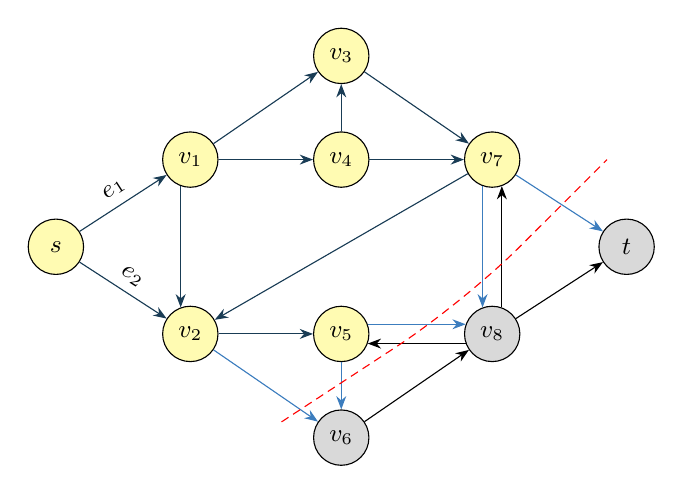
\begin{tikzpicture}[
      mycircle/.style={
         circle,
         draw=black,
         fill=yellow,
         fill opacity = 0.3,
         text opacity=1,
         inner sep=0pt,
         minimum size=20pt,
         font=\small},
      cicle_sink/.style={
         circle,
         draw=black,
         fill=gray,
         fill opacity = 0.3,
         text opacity=1,
         inner sep=0pt,
         minimum size=20pt,
         font=\small},
      myarrow/.style={
        -Stealth,
      },
      arrow_dark_blue/.style={
        -Stealth,
        fill=dark_blue,
        draw=dark_blue },
      arrow_blue/.style={
        -Stealth,
        fill=medium_blue,
        draw=medium_blue},
      arrow_red/.style={
        -Stealth,
        fill=red,
        draw=red},
        node distance=0.6cm and 1.2cm,
        xs/.style = {xshift=#1 mm},
        ys/.style = {yshift=#1 mm},
      ]
      %source
      \node[mycircle] (s) {$s$};
      
      \node[mycircle,above right=of s] (v1) {$v_1$};
      \node[mycircle,below right=of s] (v2) {$v_2$};

      \node[mycircle,right=of v1] (v4) {$v_4$};
      \node[mycircle,above=of v4] (v3) {$v_3$};
      \node[mycircle,right=of v2] (v5) {$v_5$};
      % sink
      \node[cicle_sink,below=of v5] (v6) {$v_6$};
      
      \node[mycircle,right=of v4] (v7) {$v_7$};
      % sink
      \node[cicle_sink,right=of v5] (v8) {$v_8$};
      
      \node[cicle_sink,below right=of v7] (t) {$t$};
      %\node[mycircle,right=of c4] (c5) {$v_3$};
      %\node[mycircle,below right=of c5] (c6) {$t$};

    %%% in S out S
    \foreach \i/\j/\txt/\p in {% start node/end node/text/position
      s/v1/$e_1$/above,
      s/v2/$e_2$/above,
      v1.250/v2.110//above, %.deg, .deg
      v1/v3//above,
      v1/v4//above,
      v2/v5//above,
      v3/v7//above,
      v4/v7//above,
      v7/v2//above,
      v4/v3//above}
      \draw [arrow_dark_blue] (\i) -- node[sloped,font=\small,\p] {\txt} (\j);
    
    \foreach \i/\j/\txt/\p in {% start node/end node/text/position
      v5/v6//above,
      v5.20/v8.160//above,
      v2/v6//above,
      v7.250/v8.110//above,
      v7/t//above}
     \draw [arrow_blue] (\i) -- node[sloped,font=\small,\p] {\txt} (\j); 
    
    \foreach \i/\j/\txt/\p in {% start node/end node/text/position
      v8.200/v5.340//above,
      v8.70/v7.290//below,
      v8/t//above,
      v6/v8//above}
      \draw [myarrow] (\i) -- node[sloped,font=\small,\p] {\txt} (\j);
    
    \draw[rounded corners=10mm, red, densely dashed] 
        ([xs=-4,ys=2]  v6.west)  -- ([ys=4] v8.west)   -- ([xs=11]  v7.east)
    ;

     % draw this outside loop to get proper orientation of 10
     %\draw [myarrow] (c4.250) -- node[sloped,font=\small,above,rotate=180] {10} (c2.110);
    \end{tikzpicture}
\columnbreak

	% how to draw cut line https://tex.stackexchange.com/questions/350852/directed-graph-with-cuts
	\usetikzlibrary{arrows, quotes}
	
	
	\definecolor{dark_red}{RGB}{77,16,16}
	
    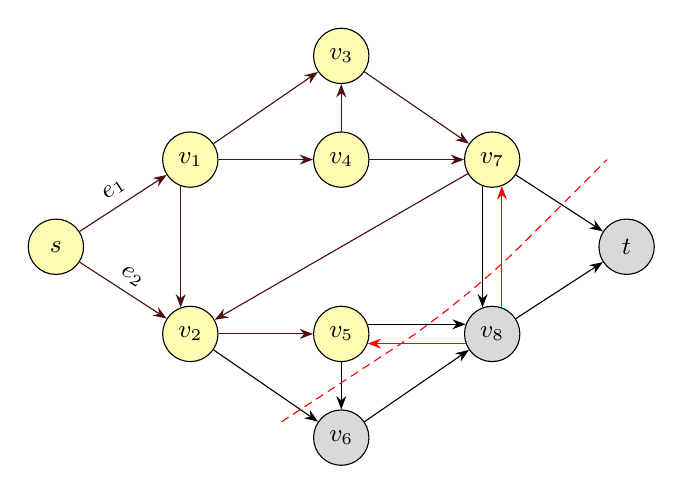
\begin{tikzpicture}[
      mycircle/.style={
         circle,
         draw=black,
         fill=yellow,
         fill opacity = 0.3,
         text opacity=1,
         inner sep=0pt,
         minimum size=20pt,
         font=\small},
      cicle_sink/.style={
         circle,
         draw=black,
         fill=gray,
         fill opacity = 0.3,
         text opacity=1,
         inner sep=0pt,
         minimum size=20pt,
         font=\small},
      myarrow/.style={
        -Stealth,
      },
      arrow_blue/.style={
        -Stealth,
        fill=blue,
        draw=blue},
      arrow_red/.style={
        -Stealth,
        fill=red,
        draw=red},
      arrow_dark_red/.style={
        -Stealth,
        fill=dark_red,
        draw=dark_red},
        node distance=0.6cm and 1.2cm,
        xs/.style = {xshift=#1 mm},
        ys/.style = {yshift=#1 mm},
      ]
      %source
      \node[mycircle] (s) {$s$};
      
      \node[mycircle,above right=of s] (v1) {$v_1$};
      \node[mycircle,below right=of s] (v2) {$v_2$};

      \node[mycircle,right=of v1] (v4) {$v_4$};
      \node[mycircle,above=of v4] (v3) {$v_3$};
      \node[mycircle,right=of v2] (v5) {$v_5$};
      % sink
      \node[cicle_sink,below=of v5] (v6) {$v_6$};
      
      \node[mycircle,right=of v4] (v7) {$v_7$};
      % sink
      \node[cicle_sink,right=of v5] (v8) {$v_8$};
      
      \node[cicle_sink,below right=of v7] (t) {$t$};
      %\node[mycircle,right=of c4] (c5) {$v_3$};
      %\node[mycircle,below right=of c5] (c6) {$t$};

    \foreach \i/\j/\txt/\p in {% start node/end node/text/position
      s/v1/$e_1$/above,
      s/v2/$e_2$/above,
      v1.250/v2.110//above, %.deg, .deg
      v1/v3//above,
      v1/v4//above,
      v2/v5//above,
      v3/v7//above,
      v4/v7//above,
      v7/v2//above,
      v4/v3//above}
      \draw [arrow_dark_red] (\i) -- node[sloped,font=\small,\p] {\txt} (\j);
    
    \foreach \i/\j/\txt/\p in {% start node/end node/text/position
      v5/v6//above,
      v5.20/v8.160//above,
      v7.250/v8.110//above,
      v7/t//above,
      v6/v8//above,
      v8/t//above,
      v2/v6//above}
      \draw [myarrow] (\i) -- node[sloped,font=\small,\p] {\txt} (\j);
     
    \foreach \i/\j/\txt/\p in {% start node/end node/text/position
      v8.200/v5.340//above,
      v8.70/v7.290//below}
      \draw [arrow_red] (\i) -- node[sloped,font=\small,\p] {\txt} (\j);
    
    \draw[rounded corners=10mm, red, densely dashed] 
        ([xs=-4,ys=2]  v6.west)  -- ([ys=4] v8.west)   -- ([xs=11]  v7.east)
    ;

     % draw this outside loop to get proper orientation of 10
     %\draw [myarrow] (c4.250) -- node[sloped,font=\small,above,rotate=180] {10} (c2.110);
    \end{tikzpicture}
\end{multicols}
\begin{proof}
\begin{align}
    \mathcal{V}(f)&=\sum\limits_{e\in out\left( s \right)}{f\left( e \right)} \tag{1}\\
    %
   &=\underbrace{\sum\limits_{e\in out\left( s \right)}{f\left( e \right)}-\underbrace{\sum\limits_{e\in in\left( s \right)}{f\left( e \right)}}_{0,\ \text{since }in\left( s \right)=\varnothing }}_{\text{from source }s\text{ to S}}+
   \underbrace{\sum\limits_{v\in S-\left\{ s \right\}}{\Bigg( \underbrace{\sum\limits_{e\in out\left( v \right)}{f\left( e \right)}-\sum\limits_{e\in in\left( v \right)}{f\left( e \right)}}_{0\text{ by conserv}\text{.}} \Bigg)}}_{\text{nodes in }S-\left\{ s \right\}} \tag{2}\\
   %
   &=\sum\limits_{v\in S}{\left( \sum\limits_{e\in out\left( v \right)}{f\left( e \right)}-\sum\limits_{e\in in\left( v \right)}{f\left( e \right)} \right)} \tag{3} \\
   %
   &=\sum\limits_{v\in S}{\sum\limits_{e\in out\left( v \right)}{f\left( e \right)}-}\sum\limits_{v\in S}{\sum\limits_{e\in in\left( v \right)}{f\left( e \right)}} \tag{4}\\
   %
   &=\sum\limits_{e\in out\left( S \right)}{f\left( e \right)}-\sum\limits_{e\in in\left( S \right)}{f\left( e \right)} \tag{5}\\
   %
   &=\left( \textcolor{dark_blue}{ \cancel{\sum\limits_{e\in out\left( S \right)\cap in\left( S \right)}{f\left( e \right)}} } +
   \textcolor{medium_blue}{\sum\limits_{e\in out\left( S \right)\cap in\left( T \right)} {f\left( e \right)} } \right)-
   \left( \textcolor{dark_red}{\cancel{\sum\limits_{e\in in\left( S \right)\cap out\left( S \right)}{f\left( e \right)}}}+
   \textcolor{red}{\sum\limits_{e\in in\left( S \right)\cap out\left( T \right)}{f\left( e \right)}} \right) \tag{6}\\
   %
   &=\textcolor{medium_blue}{\sum\limits_{e\in out\left( S \right)\cap in\left( T \right)}{f\left( e \right)}}-
   \textcolor{red}{\sum\limits_{e\in in\left( S \right)\cap out\left( T \right)}{f\left( e \right)}} \tag{7}
\end{align}
% TODO: add refs
\begin{itemize}
    \item We go from (1) to (2) by invoking the conservation of flow for all nodes $v \in S - \{s\}$, so the incoming and outgoing edges cancel each other.
    \item We go from line (2) to (3) by grouping together the external sub for all nodes including the source $s$. 
    \item We go from line (4) to (5) by rewriting the sums in a more compact way for the edges.
    \item The two diagrams colour-code the terms in (6) and (7).
\end{itemize}
\end{proof}



% ------------------------ New appendix ------------------------ %
\newpage
\subsection{Motivation for Ford Fulkerson algorithm}
\label{app:ffa_motivation}

An initial greedy approach for the maximum flow is based on the following points.

\begin{itemize}
    \item It begins by setting $f(e_i)=0$ for every $e_i \in E$.
    \item For each edge $e_i$, the capacity minus the flow $c_i - f_i$ tells us how much excess flow we can push through it. If $c_i = f_i$, then $e_i$ is saturated.
    \item It keeps finding paths (e.g. by DFS) from $s$ to $t$. When it finds a path, it pushes some \emphasis{bottleneck} flow through it, i.e. the maximum flow that its edges can carry and updates its flow. It repeats the process until there are paths where flow can be pushed, i.e. no path $P$ such that $f(e)<c(e)\ \ \forall \ \ e \in P$. 
    \item Also, then there is an $s-t$ cut $(S,T)$ with $c_i = f_i \ \ \forall \ \ e_i \in (S,T)$. By the flow value lemma (\eqref{eq:flow_value_lemma}), this will be the maximum flow we can push through an $s-t$ cut.
\end{itemize}
To be more concrete, this initial approach it can be described by the following pseudocode.
\begin{algorithm}[H] % H - use exact floating position
\caption{Maximum flow greedy algorithm 1}\label{alg:max_flow_algo_1}
\begin{algorithmic}[1]
\State \Comment{\textbf{Input:} A graph with capacities $c$, source $s$, sink $t$}
\State \Comment{\textbf{Output:} The max flow $\left| f \right|$ from $s$ to $t$}
\Procedure{GreedyMaxFlow}{$V,E,c,s,t$}
\For {$\textup{each\ \ edge\ \ }(u,v)$} \Comment{Initialisation}
\State \textbf{let} $f(u,v) \leftarrow 0$
\EndFor
\While{exists path $P$ from $s$ to $t$ in $G$ s.t. $c(u,v) - f(u,v)>0 \ \ \forall (u,v) \in P$}
\State \textbf{let} $b(P)\leftarrow \underset{\left( u,v \right)\in P}{\mathop{\min }}\,\left( c\left( u,v \right)-f\left( u,v \right) \right) $ 
\For {each edge $(u,v) \in P$}
\State $f(u,v) = f(u,v) + b$
\EndFor
\EndWhile
\State \textbf{return} $f$
\EndProcedure
\end{algorithmic}
\end{algorithm}
Let's test Algorithm \ref{alg:max_flow_algo_1} on a toy network and check whether it can actually compute the maximum flow. \\
\begin{minipage}{\linewidth}
\label{tab:greedy_alg_1_results}
\captionof{table}{A greedy maximum flow algorithm. The currently chosen path is in {\color{blue} blue}, along with the currently pushed flow ({\color{blue} blue}) and the updated ${\color{blue} \textup{flow}}/\textup{capacity}$ of each edge.} \label{tab:SVD_image_results} 
\begin{center}
\begin{tabular}{| m{.22\textwidth} | m{.22\textwidth} | m{.22\textwidth}  | m{.22\textwidth} | m{.1\textwidth} |}
\hline   
% image, rank, output, n required, norm 2 of difference, Singular value of rank r+1
    \textbf{Original} & \textbf{Iteration 1} & \textbf{Iteration 2} & \textbf{Iteration 3} & \textbf{Max flow found}\\
\hline 
\hline 
    \usetikzlibrary{arrows, quotes}
%\usepackage{xcolor}
	
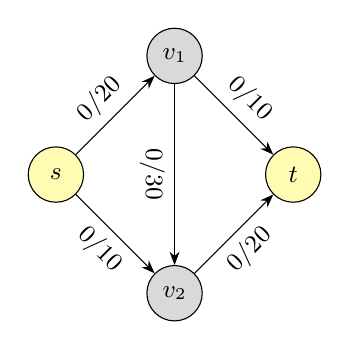
\begin{tikzpicture}[
      circle_st/.style={
         circle,
         draw=black,
         fill=yellow,
         fill opacity = 0.3,
         text opacity=1,
         inner sep=0pt,
         minimum size=20pt,
         font=\small},
       circle_node/.style={
         circle,
         draw=black,
         fill=gray,
         fill opacity = 0.3,
         text opacity=1,
         inner sep=0pt,
         minimum size=20pt,
         font=\small} ,
       arrow_black/.style={
        -Stealth,
      },
]	
      %source
      \node[circle_st] (s) {$s$};
      
      \node[circle_node,above right=of s] (v1) {$v_1$};
      \node[circle_node,below right=of s] (v2) {$v_2$};
      
      \node[circle_st,below right=of v1] (t) {$t$};

    \foreach \i/\j/\txt/\p in {% start node/end node/text/position
      s/v1/$0 \textup{/} 20$/above,
      s/v2/$0 \textup{/} 10$/below,
      v1/v2/$0 \textup{/} 30$/below,
      v1/t/$0 \textup{/} 10$/above,
      v2/t/$0 \textup{/} 20$/below}
      \draw [arrow_black] (\i) -- node[sloped,font=\small,\p] {\txt} (\j);


\end{tikzpicture} & \usetikzlibrary{arrows, quotes}
\newcommand{\bluebold}[1]{\textbf{\textcolor{blue}{#1}}} % text above = symbol

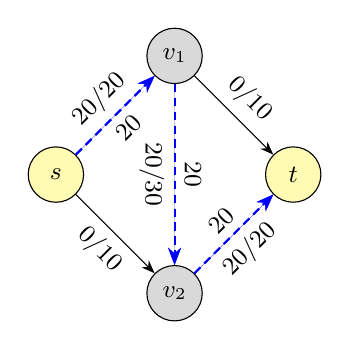
\begin{tikzpicture}[
      circle_st/.style={
         circle,
         draw=black,
         fill=yellow,
         fill opacity = 0.3,
         text opacity=1,
         inner sep=0pt,
         minimum size=20pt,
         font=\small},
       circle_node/.style={
         circle,
         draw=black,
         fill=gray,
         fill opacity = 0.3,
         text opacity=1,
         inner sep=0pt,
         minimum size=20pt,
         font=\small} ,
       arrow_black/.style={
        -Stealth,
        },
        arrow_bold/.style={
        -Stealth,
        dash pattern=on 3pt off 2pt,
        fill=blue,
        line width=0.25mm,
        draw = blue,
        }
]	
      %source
      \node[circle_st] (s) {$s$};
      
      \node[circle_node,above right=of s] (v1) {$v_1$};
      \node[circle_node,below right=of s] (v2) {$v_2$};
      
      \node[circle_st,below right=of v1] (t) {$t$};

    \foreach \i/\j/\txt/\p in {% start node/end node/text/position
      s/v2/$0 \textup{/} 10$/below,
      v1/t/$0 \textup{/} 10$/above}
      \draw [arrow_black] (\i) -- node[sloped,font=\small,\p] {\txt} (\j);
      
      \foreach \i/\j/\txt/\p in {% start node/end node/text/position
      s/v1/$\bluebold{20} \textup{/} 20$/above,
      s/v1/$\bluebold{20}$/below,
      v1/v2/$\bluebold{20} \textup{/} 30$/below,
      v1/v2/$\bluebold{20}$/above,
      v2/t/$\bluebold{20} \textup{/} 20$/below,
      v2/t/$\bluebold{20}$/above}
      \draw [arrow_bold] (\i) -- node[sloped,font=\small,\p] {\txt} (\j);


\end{tikzpicture} &  &  & 20\\
\hline 
    \usetikzlibrary{arrows, quotes}
%\usepackage{xcolor}
	
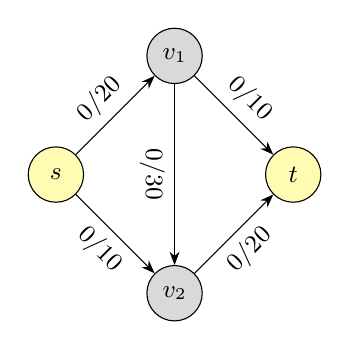
\begin{tikzpicture}[
      circle_st/.style={
         circle,
         draw=black,
         fill=yellow,
         fill opacity = 0.3,
         text opacity=1,
         inner sep=0pt,
         minimum size=20pt,
         font=\small},
       circle_node/.style={
         circle,
         draw=black,
         fill=gray,
         fill opacity = 0.3,
         text opacity=1,
         inner sep=0pt,
         minimum size=20pt,
         font=\small} ,
       arrow_black/.style={
        -Stealth,
      },
]	
      %source
      \node[circle_st] (s) {$s$};
      
      \node[circle_node,above right=of s] (v1) {$v_1$};
      \node[circle_node,below right=of s] (v2) {$v_2$};
      
      \node[circle_st,below right=of v1] (t) {$t$};

    \foreach \i/\j/\txt/\p in {% start node/end node/text/position
      s/v1/$0 \textup{/} 20$/above,
      s/v2/$0 \textup{/} 10$/below,
      v1/v2/$0 \textup{/} 30$/below,
      v1/t/$0 \textup{/} 10$/above,
      v2/t/$0 \textup{/} 20$/below}
      \draw [arrow_black] (\i) -- node[sloped,font=\small,\p] {\txt} (\j);


\end{tikzpicture} & \usetikzlibrary{arrows, quotes}
\newcommand{\bluebold}[1]{\textbf{\textcolor{blue}{#1}}} % text above = symbol

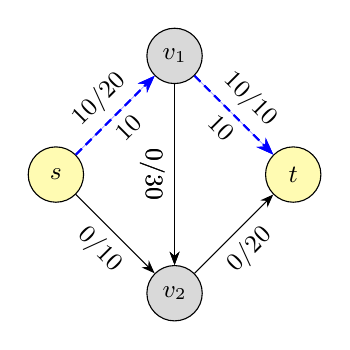
\begin{tikzpicture}[
      circle_st/.style={
         circle,
         draw=black,
         fill=yellow,
         fill opacity = 0.3,
         text opacity=1,
         inner sep=0pt,
         minimum size=20pt,
         font=\small},
       circle_node/.style={
         circle,
         draw=black,
         fill=gray,
         fill opacity = 0.3,
         text opacity=1,
         inner sep=0pt,
         minimum size=20pt,
         font=\small} ,
       arrow_black/.style={
        -Stealth,
        },
        arrow_bold/.style={
        -Stealth,
        dash pattern=on 3pt off 2pt,
        fill=blue,
        line width=0.25mm,
        draw = blue,
        }
]		
      %source
      \node[circle_st] (s) {$s$};
      \node[circle_node,above right=of s] (v1) {$v_1$};
      \node[circle_node,below right=of s] (v2) {$v_2$};
      \node[circle_st,below right=of v1] (t) {$t$};

    \foreach \i/\j/\txt/\p in {% start node/end node/text/position
      s/v2/$0 \textup{/} 10$/below,
      v1/v2/$0 \textup{/} 30$/below,
      v1/v2/$0 \textup{/} 30$/below,
      v2/t/$0 \textup{/} 20$/below}
      \draw [arrow_black] (\i) -- node[sloped,font=\small,\p] {\txt} (\j);
      
    \foreach \i/\j/\txt/\p in {% start node/end node/text/position
      s/v1/$\bluebold{10} \textup{/} 20$/above,
      s/v1/$\bluebold{10}$/below,
      v1/t/$\bluebold{10} \textup{/} 10$/above,
      v1/t/$\bluebold{10}$/below}
      \draw [arrow_bold] (\i) -- node[sloped,font=\small,\p] {\txt} (\j);



\end{tikzpicture} & \usetikzlibrary{arrows, quotes}
\newcommand{\bluebold}[1]{\textbf{\textcolor{blue}{#1}}} % text above = symbol

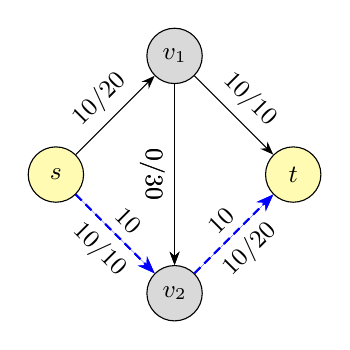
\begin{tikzpicture}[
      circle_st/.style={
         circle,
         draw=black,
         fill=yellow,
         fill opacity = 0.3,
         text opacity=1,
         inner sep=0pt,
         minimum size=20pt,
         font=\small},
       circle_node/.style={
         circle,
         draw=black,
         fill=gray,
         fill opacity = 0.3,
         text opacity=1,
         inner sep=0pt,
         minimum size=20pt,
         font=\small} ,
       arrow_black/.style={
        -Stealth,
        },
        arrow_bold/.style={
        -Stealth,
        dash pattern=on 3pt off 2pt,
        fill=blue,
        line width=0.25mm,
        draw = blue,
        }
]		
      %source
      \node[circle_st] (s) {$s$};
      
      \node[circle_node,above right=of s] (v1) {$v_1$};
      \node[circle_node,below right=of s] (v2) {$v_2$};
      
      \node[circle_st,below right=of v1] (t) {$t$};

    \foreach \i/\j/\txt/\p in {% start node/end node/text/position
      v1/v2/$0 \textup{/} 30$/below,
      v1/v2/$0 \textup{/} 30$/below,
      s/v1/$10 \textup{/} 20$/above,
      v1/t/$10 \textup{/} 10$/above}
      \draw [arrow_black] (\i) -- node[sloped,font=\small,\p] {\txt} (\j);
      
    \foreach \i/\j/\txt/\p in {% start node/end node/text/position
      s/v2/$\bluebold{10} \textup{/} 10$/below,
      s/v2/$\bluebold{10}$/above,
      v2/t/$\bluebold{10} \textup{/} 20$/below,
      v2/t/$\bluebold{10}$/above}
      \draw [arrow_bold] (\i) -- node[sloped,font=\small,\p] {\txt} (\j);


\end{tikzpicture} & \usetikzlibrary{arrows, quotes}
\newcommand{\bluebold}[1]{\textbf{\textcolor{blue}{#1}}} % text above = symbol

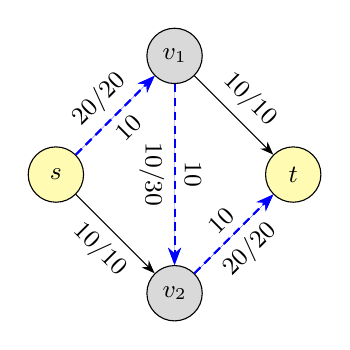
\begin{tikzpicture}[
      circle_st/.style={
         circle,
         draw=black,
         fill=yellow,
         fill opacity = 0.3,
         text opacity=1,
         inner sep=0pt,
         minimum size=20pt,
         font=\small},
       circle_node/.style={
         circle,
         draw=black,
         fill=gray,
         fill opacity = 0.3,
         text opacity=1,
         inner sep=0pt,
         minimum size=20pt,
         font=\small} ,
       arrow_black/.style={
        -Stealth,
        },
        arrow_bold/.style={
        -Stealth,
        dash pattern=on 3pt off 2pt,
        fill=blue,
        line width=0.25mm,
        draw = blue,
        }
]		
      %source
      \node[circle_st] (s) {$s$};
      
      \node[circle_node,above right=of s] (v1) {$v_1$};
      \node[circle_node,below right=of s] (v2) {$v_2$};
      
      \node[circle_st,below right=of v1] (t) {$t$};

    \foreach \i/\j/\txt/\p in {% start node/end node/text/position
      s/v2/$10 \textup{/} 10$/below,
      v1/t/$10 \textup{/} 10$/above}
      \draw [arrow_black] (\i) -- node[sloped,font=\small,\p] {\txt} (\j);
      
    \foreach \i/\j/\txt/\p in {% start node/end node/text/position
      v2/t/$\bluebold{20} \textup{/} 20$/below,
      v2/t/$\bluebold{10}$/above,
      s/v1/$\bluebold{20} \textup{/} 20$/above,
      s/v1/$\bluebold{10}$/below,
      v1/v2/$\bluebold{10}\textup{/} 30$/below,
      v1/v2/$\bluebold{10}$/above}
      \draw [arrow_bold] (\i) -- node[sloped,font=\small,\p] {\txt} (\j);


\end{tikzpicture} & 30\\
\hline

\end{tabular}
\end{center}
\end{minipage}

The maximum flow in the toy network in Table \ref{tab:greedy_alg_1_results} is $30$. However, as shown in its second row, Algorithm \ref{alg:max_flow_algo_1} does not always compute the optimal result. Choosing the path $\{(s,v_1), (v_1,v_2), (v_2,t)\}$ first uses the full capacity of edge $(v_2,t)$ so any other path from $s$ to $t$ is blocked and all the flow we can push from $s$ to $t$ is $20$. The situation can be remedied by starting from $(s,v_2)$ and pushing up to $20$ units \textit{\color{red} against} $(v_1,v_2)$. Particularly, we push $min(10,20,10)=10$. That is acceptable as long as we do not violate the original flow direction, i.e. as long as $f_{(v1,v2)}>0$.\\
This reconsidered algorithm avoids such flow blocks and its iterations are presented in the table below. It is able to find the optimal maximum flow.

\begin{minipage}{\linewidth}
\label{tab:greedy_alg_1_results}
\captionof{table}{The revisited greedy maximum flow algorithm. The currently chosen path is in {\color{blue} blue}, along with the currently pushed flow ({\color{blue} blue}) and the updated ${\color{blue} \textup{flow}}/\textup{capacity}$ of each edge.} 
\begin{center}
\begin{tabular}{| m{.22\textwidth} | m{.22\textwidth} | m{.22\textwidth}  | m{.22\textwidth} | m{.1\textwidth} |}
\hline   
% image, rank, output, n required, norm 2 of difference, Singular value of rank r+1
    \textbf{Original} & \textbf{Iteration 1} & \textbf{Iteration 2} & \textbf{Iteration 3} & \textbf{Max flow found}\\
\hline 
\hline 
    \usetikzlibrary{arrows, quotes}
%\usepackage{xcolor}
	
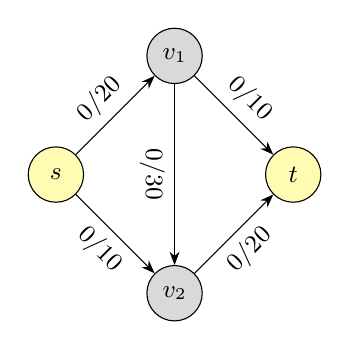
\begin{tikzpicture}[
      circle_st/.style={
         circle,
         draw=black,
         fill=yellow,
         fill opacity = 0.3,
         text opacity=1,
         inner sep=0pt,
         minimum size=20pt,
         font=\small},
       circle_node/.style={
         circle,
         draw=black,
         fill=gray,
         fill opacity = 0.3,
         text opacity=1,
         inner sep=0pt,
         minimum size=20pt,
         font=\small} ,
       arrow_black/.style={
        -Stealth,
      },
]	
      %source
      \node[circle_st] (s) {$s$};
      
      \node[circle_node,above right=of s] (v1) {$v_1$};
      \node[circle_node,below right=of s] (v2) {$v_2$};
      
      \node[circle_st,below right=of v1] (t) {$t$};

    \foreach \i/\j/\txt/\p in {% start node/end node/text/position
      s/v1/$0 \textup{/} 20$/above,
      s/v2/$0 \textup{/} 10$/below,
      v1/v2/$0 \textup{/} 30$/below,
      v1/t/$0 \textup{/} 10$/above,
      v2/t/$0 \textup{/} 20$/below}
      \draw [arrow_black] (\i) -- node[sloped,font=\small,\p] {\txt} (\j);


\end{tikzpicture} &
    \usetikzlibrary{arrows, quotes}
\newcommand{\bluebold}[1]{\textbf{\textcolor{blue}{#1}}} % text above = symbol

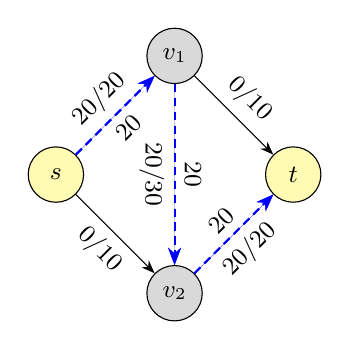
\begin{tikzpicture}[
      circle_st/.style={
         circle,
         draw=black,
         fill=yellow,
         fill opacity = 0.3,
         text opacity=1,
         inner sep=0pt,
         minimum size=20pt,
         font=\small},
       circle_node/.style={
         circle,
         draw=black,
         fill=gray,
         fill opacity = 0.3,
         text opacity=1,
         inner sep=0pt,
         minimum size=20pt,
         font=\small} ,
       arrow_black/.style={
        -Stealth,
        },
        arrow_bold/.style={
        -Stealth,
        dash pattern=on 3pt off 2pt,
        fill=blue,
        line width=0.25mm,
        draw = blue,
        }
]	
      %source
      \node[circle_st] (s) {$s$};
      
      \node[circle_node,above right=of s] (v1) {$v_1$};
      \node[circle_node,below right=of s] (v2) {$v_2$};
      
      \node[circle_st,below right=of v1] (t) {$t$};

    \foreach \i/\j/\txt/\p in {% start node/end node/text/position
      s/v2/$0 \textup{/} 10$/below,
      v1/t/$0 \textup{/} 10$/above}
      \draw [arrow_black] (\i) -- node[sloped,font=\small,\p] {\txt} (\j);
      
      \foreach \i/\j/\txt/\p in {% start node/end node/text/position
      s/v1/$\bluebold{20} \textup{/} 20$/above,
      s/v1/$\bluebold{20}$/below,
      v1/v2/$\bluebold{20} \textup{/} 30$/below,
      v1/v2/$\bluebold{20}$/above,
      v2/t/$\bluebold{20} \textup{/} 20$/below,
      v2/t/$\bluebold{20}$/above}
      \draw [arrow_bold] (\i) -- node[sloped,font=\small,\p] {\txt} (\j);


\end{tikzpicture} &
    \usetikzlibrary{arrows, quotes}
\newcommand{\bluebold}[1]{\textbf{\textcolor{blue}{#1}}} % text above = symbol

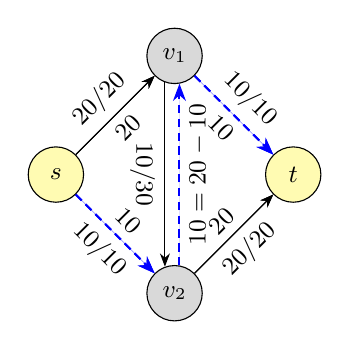
\begin{tikzpicture}[
      circle_st/.style={
         circle,
         draw=black,
         fill=yellow,
         fill opacity = 0.3,
         text opacity=1,
         inner sep=0pt,
         minimum size=20pt,
         font=\small},
       circle_node/.style={
         circle,
         draw=black,
         fill=gray,
         fill opacity = 0.3,
         text opacity=1,
         inner sep=0pt,
         minimum size=20pt,
         font=\small} ,
       arrow_black/.style={
        -Stealth,
        },
        arrow_bold/.style={
        -Stealth,
        dash pattern=on 3pt off 2pt,
        fill=blue,
        line width=0.25mm,
        draw = blue,
        },
        arrow_bold_dashed/.style={
          -Stealth,
          dash pattern=on 3pt off 2pt,
          fill=blue,
          line width=0.25mm,
          draw=blue,
        }
]	
      %source
      \node[circle_st] (s) {$s$};
      
      \node[circle_node,above right=of s] (v1) {$v_1$};
      \node[circle_node,below right=of s] (v2) {$v_2$};
      
      \node[circle_st,below right=of v1] (t) {$t$};

    \foreach \i/\j/\txt/\p in {% start node/end node/text/position
      s/v1/$20 \textup{/} 20$/above,
      v1.250/v2.110/$\bluebold{10}\textup{/} 30$/below,
      v2/t/$20$/above,
      s/v1/$20$/below,
      v2/t/$20 \textup{/} 20$/below}
      \draw [arrow_black] (\i) -- node[sloped,font=\small,\p] {\txt} (\j);
      
    \foreach \i/\j/\txt/\p in {% start node/end node/text/position
      s/v2/$\bluebold{10} \textup{/}10$/below,
      s/v2/$\bluebold{10}$/above,
      v1/t/$\bluebold{10} \textup{/} 10$/above,
      v1/t/$\bluebold{10}$/below}
      \draw [arrow_bold] (\i) -- node[sloped,font=\small,\p] {\txt} (\j);
    \foreach \i/\j/\txt/\p in {% start node/end node/text/position
      v2.80/v1.280/$\bluebold{10=20-10}$/below}
      \draw [arrow_bold_dashed] (\i) -- node[sloped,font=\small,\p] {\txt} (\j);


\end{tikzpicture}  &  & 30\\
\hline 

\end{tabular}
\end{center}
\end{minipage}

Therefore finding the augmented in Algorithm \ref{alg:max_flow_algo_1} can be fixed as follows. Suppose we want to traverse an edge $(u,v)$ with flow $f$ and capacity $c$. If we traverse $u\rightarrow v$ we can push up to $c-f$ extra units and if we traverse $v\rightarrow u$ we can push up to extra $f$ units from $v$ to $u$, or equivalently subtract $f$ units from $u$ to $v$. This motivates us to define the \emphasis{residual graph}, which is a function of the original graph $G$ and its flow $f$. 




% ------------------------ New appendix ------------------------ %
\newpage
\subsection{Ford Fulkerson source code}
\label{app:ffa_code}

The network class along with the algorithm implementation \TODO[ref: \url{https://github.com/bigbighd604/Python/blob/master/graph/Ford-Fulkerson.py}]:
\inputminted{python}{src/ford-fulkerson/class_network.py}
And the driver code:
\inputminted{python}{src/ford-fulkerson/main.py}

% ------------------------ New appendix ------------------------ %
\newpage
\subsection{Ncuts source code}
\label{app:ncuts_code}
\inputminted{python}{src/ncuts/ncuts.py}

% ------------------------ New appendix ------------------------ %
\newpage
\subsection{Snakes using \mintinline{python}{scikit-image} source code}
\label{app:snakes_code}
\inputminted{python}{src/snakes/snakes.py}

% ------------------------ New appendix ------------------------ %
\newpage
\subsection{Snakes from scratch, greedy minimisation}
\label{app:my_snakes_code}
\inputminted{python}{src/snakes/mysnake.py}

% ------------------------ New appendix ------------------------ %
\newpage
\subsection{K-means written from scratch}
\label{app:src_my_kmeans}
The code uses a small utility module named \mintinline{python}{my_k_plots} to plot points  listed below:
\inputminted{python}{src/kmeans/my_k_plots.py}
Below is the functionality with the driver code:
\inputminted{python}{src/kmeans/my_k_means.py}

% ------------------------ New appendix ------------------------ %
\newpage
\subsection{K-means in OpenCV}
\label{app:src_kmeans_opencv}
The code below demonstrates an application on some 2D data and on an RGB (read as BGR) image.
\inputminted{python}{src/kmeans/k_means_cv.py}


% ------------------------ New appendix ------------------------ %
\newpage
\subsection{Watershed workflow 1 source (little overlap)}
\label{app:watershed_workflow_1}
To run this example, simple execute the script below with no arguments.
\inputminted{python}{src/watershed/watershed_dt.py}


% ------------------------ New appendix ------------------------ %
\newpage
\subsection{Watershed workflow 2 source (large overlap)}
\label{app:watershed_workflow_2}
To run this example, simple execute the script below with no arguments.
\inputminted{python}{src/watershed/watershed_morph.py}





%%%%%%%%%%%%%%%%%%%%%%%%%%%%%%%%%%%%%%%%%%%%%%%%%%%%%%%%%%%%%%%%%%%%%%%%%%%%%%%%%%%%%%%%%%%%%%%%%%%%
% REFS
%%%%%%%%%%%%%%%%%%%%%%%%%%%%%%%%%%%%%%%%%%%%%%%%%%%%%%%%%%%%%%%%%%%%%%%%%%%%%%%%%%%%%%%%%%%%%%%%%%%%
\newpage
\printbibliography




\end{document}
